

\let\cleardoublepage\clearpage


\chapter{Introduction}

Despite living in a highly developed world, food security is still a prevailing issue. Around 842 million people are estimated to be experiencing malnourishment and hunger \footnote{http://www.fao.org/news/story/en/item/204232/icode/}. Especially global soaring food prices seem to have a negative effect by transmitting into rising food inflation rates in domestic markets \cite{Tadesse2014}. The consequences of rising food prices differ among developed and developing countries. Developing countries struggle with accessibility due to poor infrastructure and affordability as most of their income is spent on food. Developed countries on the other hand face increased malnourishment and as a result an increase of health-related diseases such as obesity or diabetes \footnote{http://www.fao.org/docrep/u9920t/u9920t07.htm}.  The diversity between and within different countries calls for an improved approach in effectively tracking long-term development trends to aid the development of safer policies and ultimately a world where everybody has enough food. 

Food security assessments are typically done through household surveys, which are timely and expensive to execute \cite{deCastro91}. It takes years to analyse, validate and release. As a result, it is mostly an exercise in history, they fail to provide real time information which hinders an early response \cite{ungp2013}. Today however we live in a world where multimedia content is rapidly increasing \cite{twitter13}, especially as people continuously use social networks for communicating and documenting their lives. More often then not social media provides a rich source of media content such as images and links to news \cite{twitter13}. As people use those services they leave traces in the data and if their lives change for the better or the worse we see those patterns change as well \cite{adeline14}. As a result social media successfully mirror the well being of our society \cite{van2012conversation}. 

Twitter is considered to be one of the largest social media platforms and among one of the most consistent and prevalent topics on the platform is food \footnote{http://www.businessinsider.com/most-discussed-topics-on-social-media-2013-5}. Cleaned and aggregated this provides a valuable opportunity for \emph{studying food security indicators on Twitter}. Previous research  \cite{ungp2013} and commercial applications \footnote{http://foodsecurity.dupont.com/2014/10/09/the-need-for-a-common-language-to-support-global-food-security/} in this are have focused on visualising the data but do not provide and in-depth investigation of the forecasting capabilities. Understanding if and how food security objectives are perceived by the population and whether the information is predictive of future price changes or even indicative of the next food crisis is the focus of this work. This dissertation contributes to the community by providing a fully automatic forecasting approach for food prices. 

\newpage 

%The recent food crisis in 2011 has driven 100 of millions into extreme poverty causing riots, falling markets and collapsing governments as experienced during the 2011 revolution that swept the middle east \footnote{http://www.globalissues.org/article/792/mideast-north-africa-unrest}. 


First, and most central to this dissertation we try to understand how social media users talk about food security indicators. This inherently comes down to finding contextually similar words to our given food security objectives. Most frequently a local co-occurence analysis is performed \cite{AbbarMW14}, however in this work we make a case that this approach fails to capture a lot of indicative terms \cite{burgess98}. Hence, we model the language used in Twitter to refer to food products and food security indicators by using a semantic space of words co-occurrences (\S\ref{hal}) and propose a set of metrics that favour the semantic analysis of social media text  (\S\ref{hal_result}). Ultimately, with this analysis, we seek to distinguish between relevant and irrelevant discussions on social media. The analysis of the retrieved tweets showed that raw products (e.g. \emph{corn}) are only very sparsely represented in Twitter conversations (\S\ref{food_lex}). To circumvent this problem we use a mixture of manual annotation and automated vocabulary expansion to increase the coverage of our lexicon (\S\ref{food_lex},\S\ref{pred_lex} ).

In a second study we investigate whether social media captures useful signals about food price fluctuations. To address this questions we performed a large-scale analysis of 29M Tweets distributed over 15.5 million users. We investigate to what extent the volume of food discussions can be correlated to the international Food Price Index and commodity price quotes (\S\ref{core}). We found that on an aggregated level (e.g. meat) no real correlation exists however on a finer granularity (e.g. sirloin steak) certain products exhibit a strong linear relationship of up to 0.7369 with a significance of 0.0001. Considering this evidence we apply a methodology introduced by \cite{olt15} to automatically detect peaks in volume of the twitter data and investigate the relevance to our desired food security objectives. The results showed that up to 13 \% of the peaks can be attributed to discussions around food supply, price and poverty (\S\ref{final_result}). 

In a third analysis we seek to understand if it is possible to use social media to model commodity prices. Being able to forecast price trends is of great importance as it is widely assumed that  the food crisis in 2008 was accelerated by speculative actions on the commodity future markets \cite{foodwatch}. The prices of U.S. corn tripled from \$94 to \$281 during a period of only three years. With a Pearson correlation of 0.8436 and a significance of 0.0001 there is a strong correlation  between the Food Security Index and the commodity prices making it an important indicator. We hence monitor volatile commodity prices by using an Adaptive neuro fuzzy inference system for time series modelling (\S\ref{fuzzy_model}). We show that social media features by itself are not informative enough of explaining the price variance. However, coupled with price data we are able to accurately predict a trend four weeks into the future (\S\ref{fuzzy_model}). 

Overall this dissertation demonstrates the potential value of a large scale twitter analysis for monitoring food security. We believe there are a range of applications for governmental institutions, healthcare and the private sector alike.  In the next Chapter \ref{2} we present similar work to ours. In Chapter \ref{3} we perform an investigation of the word semantics and detail a framework for creating our lexicons.  In Chapter \ref{4} we perform a correlation analysis between the tweet volume and the international Food Price Index. Chapter \ref{5} details the time series modelling of different commodities. Lastly, in Chapter \ref{6} we conclude our findings and give directions for future work. 





\chapter{Literature Review}
\label{2}

Relevant work was performed in the fields of economics, social development, predicting real world quantities through text data and the study of dietary patterns. We review each of them and lastly detail work similar to ours. 

Following the two recent food crises in 2007 and 2010 a lot of research in economics has been centered around defining causes of volatile food prices \cite{irwin} \cite{manuelbeyond}. Getaw Tadesse et. al. \cite{Tadesse2014}  defined a taxonomy for drivers of  international food price spikes and differentiated among three different causes namely exogenous shocks, conditional causes and internal causes. Examples of exogenous shocks are extreme weather events, oil price shocks, economic and demand/supply growth, and lastly economic shocks. Conditional causes can originate through political conflict or market conditions. Internal causes on the other hand are speculative activities (driven by price expectations) and declines in world food stocks. Contrary to our work most of these studies try to find causal links between official statistics of oil inflation rates, supply growth and the food price mostly neglecting public sentiment or some quantifiable measure of current affairs (e.g. news). Through the use of Twitter we try to capture the above mentioned indicators and extend on previous studies by investigating the effect of  public sentiment on volatile food prices.

Studies on social development investigated how twitter users react during a food crisis and if social media could be used as a tool for food risk communication. Rui Gaspar et. al. \cite{Gaspar14} performed an extensive study on Twitter communication during the 2011 European EHEC outbreak. They investigated the response of a population when coping with food-related threats. Their findings showed that most people were seeking for information and showed a high degree of uncertainty but also anger was expressed in regards of identifying the contaminated products. Peter Rutsawert et. al. \cite{so90610} analysed Social Media as a tool for risk communication. Most notably they examine the risks and benefits of such a medium. The experts interviewed for this study mostly agreed that social media is a valuable tool for food crisis communication as it allows to speed up correspondences and provides a platform for interaction. Furthermore they found it to be helpful in understanding public concerns. The most noted objection was that social media might act as an amplifier an escalate a food crisis. Recently a new medium for monitoring social development has emerged. With a mobile phone coverage of more then 90 \% in most developing countries mobile phone data has shown to be a valuable indicator for socio-economic problems.  Adeline Decuyper et al. \cite{adeline14} correlate the airtime credit purchases to the expenditure on vegetable. People that spend more money on their mobile phones also spend more money on food. This was shown to be true with a Pearson correlation of  over 0.8. 

Our work falls into the broader scope of predicting real world quantities through text data. A lot of work has focused on predicting movie box-office revenues due to its high attention on social media. Sitaram Asur et al. \cite{Asur10} showed that twitter outperformed market-based predictions for box-office revenues through a regression model based on twitter volume and sentiment of reviewers. Further examples followed for elections. Andranik Tumasjan et al.'s  \cite{tumasjan2010} prediction results were very similar to  traditional election poll's accuracy by simply counting the occurrence of the candidates in tweets. Current work has focused on predicting economic and market trends by leveraging social media \cite{xue12} \cite{de08} \cite{Si_exploitingtopic}. While this work generates a lot of attention in the communist its applications for trading purposes remain unknown \cite{sentiment2014}. Similar to above work we use the attention and sentiment of twitter to explain the variance of a known quantity but juxtapose the problem to the topic of food security to understand how to use words in a specific context to predict a measurable quantity. 

Natalie Dixon \cite{dixon} build the foundation for relating tweets about food to known quantities. She analysis global food consumption patterns and  tries to understand how certain items are perceived by the population and how the consumption of food differs between countries. In her work she makes assumptions about how food about twitter could be predictive for official GDP statistics and obesity levels. The later was investigated by Sofiane Abbar et. al. \cite{AbbarMW14}. By assigning specific nutritional values (calories) to each food item mentioned in a tweet they aggregate the caloric intake per state and correlate it with the official obesity and diabetes rates. A strong correlation was observed of r = 0.77 for obesity and r 0.66 for diabetes. This paper makes a strong case on the potential value of twitter as a national surveying tool. Further studies on dietary patterns were performed by Robert West et. al. \cite{west2013}. Web logs of receipes were investigated to study the dietary preferences of a population. They found a siginificant correlation between the sodium intake displayed in those logs and the number of congestive heart failures reported at the hospital. 

Only a few studies have been performed for food and price. Victor Chahuneau et al. \ref{Chahuneau12} studies how the semantics of menus affect the price. In other words what kind of language is indicative of a cheap or expensive menu. They further explore the relationship between the sentiment of a restaurant reviews and the menu price. For instance they showed that menus containing words indicative of locally-grown food are more expensive then menus containing words appealing to tradition (old time favourite, real, fashioned). Lastly, the work by the UN  \cite{ungp2013} which is most similar to ours illustrates how Twitter reflects changes in food prices. In their analysis the tweet load was correlated to a time series of food prices. Observations showed that there is a linear relationship between food and tweet increase. One of the main conclusions was that despite a strong correlation domain knowledge is needed as speculations sometimes cause the public to panic causing false positives. 

Our work extends the above analysis to a range of different foods not only considering the raw materials but also resulting products which are more present in social media. Lastly we do not make any hypothesis about what could have caused the attention spikes but perfume a detailed investigation of the content causing the fluctuations in twitter volume. Although the UN showed the potential in twitter as an indicator of food security no actions have been taken to predict real world quantities. 




\chapter{Social Media Data Acquisition}
\label{3}

The topic food is discussed in many contexts on social media. To distinguish the relevant from the unrelevant Tweets we follow a framework illustrated in Figure \ref{fig:lex_arch}. Although food security objectives are well defined it is a challenging task to filter Tweets that fall into such segments. We hence motivate and provide an overview of a semantic analyser HAL  \cite{lund96}. After filtering Twitter data with an initial list of food related terms  (e.g. \emph {rice, wheat, milk})  we proceed to use HAL to increase the number of food related keywords that eventually build our food lexicon. In a second round we collect Twitter data corresponding to the food lexicon and use it as a corpus to study the semantics of the terms price, supply, poverty and needs. We perform the analysis on a number of different random samples and experiment with different configurations of the algorithm HAL. The resulting keywords of the semantic analyser are presented to crowd workers which accept or reject terms based on a set of instructions. Finally the accepted terms (e.g. \emph{pricey}, \emph {cheap}, \emph{available}) build the predictor lexicon which aims to capture Tweets that are relevant to food security. We downloaded 2 TB of Tweets from the internet archive \footnote{https://archive.org/details/archiveteam-json-Twitterstream}  over a span of October 2011 - September 2014.  The filtering process detailed in the last section of this chapter resulted with 29 M food relevant Tweets which corresponds roughly to 4.5 \% of the entire sample.



%In this chapter, we describe how we filtered for relevant Tweets using two different lexicons. The food lexicon contains keywords with food related terms where the predictor lexicon contains terms with factors influencing the price and supply of the goods (e.g. \emph{pricey}, \emph {cheap}, \emph{available}). 
%Firstly we motivate and detail an algorithm Hyperspace Analogue to Language (HAL)  \cite{lund96} for candidate term selection. We then  experimentally evaluate the  different metrics influencing the performance of HAL, discuss different frameworks for selecting candidate terms for our food, respectively predictor lexicon and lastly explain the filtering process of the Tweets. 



%In Figure \ref{fig:lex_arch} we illustrate our methodology for candidate term selection and data sampling which we discuss in this chapter. First in Section \ref{hal} we motivate and detail an algorithm Hyperspace Analogue to Language (HAL) that we use for our term selection  \cite{lund96}. In Section \ref{food_lex} we filter Twitter data with an initial list of food terms and proceed to use a semantic analyser on a  set of Tweets to find contextually similar words to the term food. Only if the semantically similar terms agree with a set of well defined rules the authors of this thesis add the terms together with a list of food product terms to the food lexicon. In Section \ref{pred_lex} we collect Twitter data corresponding to the food lexicon and use it as a corpus  to study the semantics of the terms price, supply, poverty and needs. The results are presented to crowd workers which accept or reject terms based on a set of instructions. We analyse the results of the algorithm HAL along and evaluate the crowd task in later sections. Last,  we discuss the different filtering methods applied as applied in the Image bellow. 
\begin{figure}[H]
        \centering
         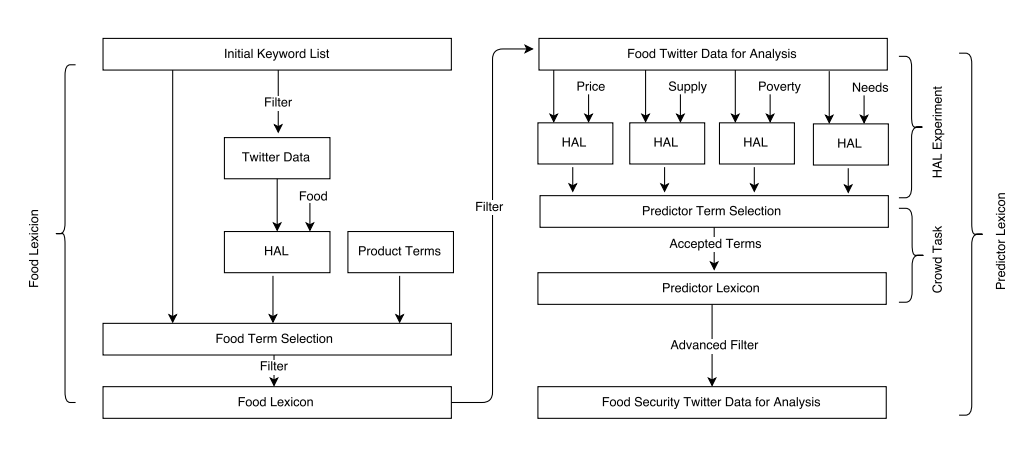
\includegraphics[width=1\textwidth ]{img/lex/lexica_architecture}
              
        \caption{Framework of the Social Media Data Acquisition}
        \label{fig:lex_arch}
\end{figure}








\section{Hyperspace Analogue to Language}
\label{hal}

\say{HAL creates a semantic space from word co-occurrences} \footnote{https://code.google.com/p/airhead-research/wiki/HyperspaceAnalogueToLanguage}. By using a sliding window parsing mechanism, the frequency of each term co-occurring within a fixed window size is recorded.  It is important to note that HAL only records the terms before the word we wish to analyse the context from. The terms after the word will appear in the column in the matrix that corresponds to that word.  The matrix is created by storing a vector for each word with the number of co-occurrences of every other word in the corpus. Hence, if our corpus contains $N$ different words the resulting HAL space would be a square matrix of co-occurrences. Every time a specific word appears in the fixed window size the co-occurrence vectors are updated. For each co-occurrence, HAL applies a scoring function. Words that appear closer receive an inversely proportional score to its distance.

 To illustrate the idea \cite{burgess98} gives an example of a simple sentence \emph {The horse raced past the barn fell.} in Table \ref{tab:halex} with a sliding window of five. Let us consider the first row.  \emph{The} precedes \emph{Barn} twice. Once within a distance of five and the other time it directly precedes the word  \emph{Barn}. Hence, that cell receives a score of five for the proximate one and a score of one for the word further away resulting in a final score of six. 

Following the creation of the matrix we concatenate both the column and row vector of a word, where the former represents the preceding words and the later the following. To compare the distance of the vectors we used the cosine similarity function. 


\begin{table}[H]
\centering
\begin{tabular}{ c c c c c c c} \toprule
  & Barn & Fell & Horse &  Past & Raced & The \\ 
  \hline
 Barn &  & & 2 &  4 & 3 & 6 \\ 
 Fell & & 5 & 1 &  3 & 2 & 4 \\ 
 Horse & & &  &   &  & 5 \\ 
 Past & & & 4 &   & 5 & 3 \\ 
 Raced & &  & 5 &   &  & 4 \\ 
 The & &  & 3 &  5 & 4 & 2 \\ 
   \bottomrule
\end{tabular}
\caption{Toy example of HAL}
\label{tab:halex}
\end{table}









\subsection{Motivating a Semantic Approach}
\label{subsec:hal}

HAL allows us to study the relationship between words. More specifically it is an algorithm that aids our goal of understanding what words are represented in the context of \emph{food} and topics targeted around \emph{food security}. To achieve this target we need a methodology for representing the meaning of a word. We analyse the context of a word to identify new words that have a similar meaning or given an identical context express the same thing. The later is concerned with identifying synonyms where as the former looks at the contextual similarity. For example, let us look at the word \emph {mould} and \emph {tons}. Those two words seem unrelated, but given the context of food they express the same thing.  Namely an abundance of food. Burgess and Lund \cite{burgess98} motivate that through the context,  they possess elements of item's similarity but by themselves they would never be considered words with similar meaning. Burgers and Lund further note that the words are not similar because they occur frequently locally, but because they occur frequently in similar sentential context. They further argue  that a simple local co-occurrence analysis misses to capture a lot of relationships. For example the word street and road are basically synonyms, however they seldom locally co-occur. Road and street do however occur in the same context. Those observations motivated us to deviate from the commonly used co-occurrence analysis and take a step further to improve the precision of our filtering framework. 




\begin{comment}
\subsection{Discussion}

We observed that HAL has a good precision given a high similarity threshold. For the top 20 keywords we evaluated a precision of 100 \% for food relevant terms. In the top 20 we found other food items building the majority of the retrieved words. However, the precision varies with the window and sample size. These variables, as our evaluation has shown, are very much dependent on the form of the corpus.  

With decreasing similarity HAL highlighted some topics indirectly associated with food security. For example there was a high percentage of country names that showed a clear association with food. Where the majority of the retrieved countries such as Thailand, Bali \footnote{http://www.nomad4ever.com/2008/08/24/top-10-popular-foods-of-asia-explained/} or the cities Singapore and Paris \footnote{http://www.hellotravel.com/stories/best-food-cities-in-world} are considered to be famous holiday destinations for food lovers other retrieved countries such as Pakistan, Syria, Jakarta India or the Philippines \footnote{http://foodsecurityindex.eiu.com/Country} are cities with a history of food insecurity and political unrest. 
\end{comment}



\section{Food Lexicon}
\label{food_lex}

We began the construction of our Food Lexicon by considering  a simple list of food related keywords. To avoid ambiguities we will refer to the initial list of keywords as $K_{initial}$. Words included are the most common traded food commodities as listed by IMF \footnote{http://www.imf.org/external/np/res/commod/index.aspx} along the ten most important staple foods that feed the world \footnote{http://knowledge.allianz.com/demography/health/?767/the-worlds-staple-foods}. 

We filtered the archive dataset using exact string matching on $K_{initial}$. The distribution of the food related Tweets motivated us to structure our lexicon hierarchically as certain commodities were only represented very sparsely and insufficient for further analysis. Where global keywords such as \emph{food} are highly represented, more specific keywords such as \emph{beef} occur infrequently. To circumvent this problem, we mimic the hierarchical representation of the Food and Argriculture Organisation of the United Nations (FAO)  \footnote{http://www.fao.org/worldfoodsituation/foodpricesindex/en/}. 

FAO tries to measure the overall food fluctuation by five different food categories namely \emph{meat, dairy products, cereals, vegetable oil} and \emph {sugar}. We further created a category named \emph{Other Food of Interest}. This category contains general keywords (e.g. \emph{food, dinner or lunch}) and food keywords that cannot be assigned to one of the five categories, but frequently occur (e.g. \emph {coffee, tea}). To be considered frequent,  the set of Tweets containing the keyword needs to be $> 1\%$ of the total sample. \emph{meat, dairy, cereals, vegetable oil, sugar} and \emph{other food of interest} build the top layer of our hierarchical representation as shown in Figure \ref{fig:food_lex} (only a subset of the lexicon is displayed). 

For the second layer we use subcategories. As the name implies  subcategories abstract the categories into different subsets i.e. for \emph{meat} we would have the subsets \emph{beef, chicken, lamb} and \emph{pork}. 

As the third layer and lowest instance, we consider food products. Each subcategory consists of food items which \textbf{i.)} can simply be the name of a category and subcategory (e.g. \emph{meat, beef}) or  \textbf{ii.)} be a product that is commonly found in markets and stores around the world. An example of the later would be \emph{flour} for the subcategory \emph{wheat}. The intuition and motivation to include such products is simple. Firstly, we were motivated to include such terms because products are more likely to capture the social attention than raw items due to their every day use. For our second argument let us consider the production of the product pasta. The variable cost factors are the raw materials flower and egg, machinery maintenance and the cost of the packaging. Where maintenances are performed on a regular predictable basis the raw materials plastic, egg and flower are market driven.  \footnote{$http://www.wikinvest.com/stock/Fomento_Economico_Mexicano_S.A.B._de_C.V._(FMX)/Increases_Prices_Raw_Materials_Increase_Coca-cola_Femsas_Cost$}. If the price of the raw materials increase then it is very likely that the price of pasta will increase as well.  Products should hence be just as expressive in explaining the variance of food prices. One however has to be cautious as certain producers hedge themselves against price fluctuations of commodities allowing them to sell the product to the same price despite rising commodity prices. 
\begin{figure}[H]

\Tree[.{FoodLexicon} [.{Meat} [.Beef \textit{Steak} ] ]
          [.Dairy [.Cheese \textit{Mozzarella} ]
                [.Milk \textit{Cream}  ]]
                [.Cereals [.Wheat \textit{Flour} ]
                [.Corn  \textit{Whisky}  ]     ]
                [.{Vegetable Oil} [.Soya \textit{Soybean Oil} ]]
                [.{Other Food of Interest} [.Fish \textit{Salmon} ]]]

\caption{Food Lexicon - Hierarchy}\label{fig:food_lex}
\end{figure}


 Other than the sparsity of the data we further faced the problem of ambiguous keywords. \emph {Soy} is such a keyword that refers in English to the \emph{bean} and in Spanish to the verb \emph{to be}. To avoid such ambiguity we extended the term to make it distinct (e.g. \emph{soy} $\to$  \emph{soy bean}). Terms were added to the lexicon by following a framework as explained in the following section. 



\subsection{Candidate Food Term Selection}

We initially assume an empty set $K_{final}$ and structure it hierarchically as mentioned in the previous section. The six categories ($c_1, c_2 ... c_6)$ are $\in K_{final}$ where $c_i$ is one of the six categories mentioned above. For interpretability purposes we introduce an axiom in form of a set $K_{all}$. It only contains five of the above mentioned six categories \emph{meat, dairy products, cereals, vegetable oil, sugar} excluding the category \emph{other food of interest}. We assume that $K_{all}$ is a fully populated lexicon containing all possible food items for a specific category (e.g. the subset dairy would contain all possible dairy products). It returns $True$ if a term is an element of the set and $False$ otherwise. For all keywords $k_i \in K_{initial}$ we evaluate if $k_i\in K_{all}$. If $True$ we add $k_i$ to $K_{final}$. For all keywords $k_i \notin K_{all}$ the condition of it being frequent is evaluated and if $True$ we add it to the category \emph{other food of interest} $c_6 $ in $K_{final}$.  Infrequent terms were discarded (e.g. \emph {orange, cocoa, onion}). Lastly, the set $K_{final}$  was further enriched by using food terms of products (e.g. \emph{pasta, flower}), let's call those terms $p_i$, that have been identified by \cite{AbbarMW14}. Again we only add $p_i$ to $K_{final}$ if it is clearly a meat, dairy, sugar, oil or cereal product or in other words an element of $K_{all}$. To further improve our coverage of the six food categories we filtered for synonyms and contextual similar words using HAL. 

We summarize our framework as follows: 

\begin{description}
  \item[1.)] Add all keywords $k \in K_{initial}$ to  $K_{final}$ only if $k \in K_{all} $ or $k$ is frequent 
  \item[2.)] Include all $p_i$ to $K_{final}$ only if $p_i \in K_{all}$
  \item[3.)] Create a HAL space using a random subsample of 10\% from $K_{initial}$ with all keywords that occur $> 100$. $\forall c_i \in K_{final} $  pick the keyword $k\in K_{final}$ that most frequently occurs over the entire sample and retrieve the top 500 terms with the highest vector similarity in the HAL space. The authors hand select those that are $\in K_{all}$ and add it to $K_{final}$.
\end{description}

\begin{comment}
As noted in \textbf{3.)} the authors of this dissertation manually select the relevant terms retrieved by HAL. The most frequent term in our corpus was found to be \emph{food} and words with a high vector similarity were other food keywords building the clear majority of the retrieved terms. Words that we rejected from HAL were mostly terms indirectly associated with food. For example there was a high percentage of country names that showed a clear association with food. Where the majority of the retrieved countries such as Thailand, Bali \footnote{http://www.nomad4ever.com/2008/08/24/top-10-popular-foods-of-asia-explained/} or the cities Singapore and Paris \footnote{http://www.hellotravel.com/stories/best-food-cities-in-world} are considered to be famous holiday destinations for food lovers other retrieved countries such as Pakistan, Syria, Jakarta India or the Philippines \footnote{http://foodsecurityindex.eiu.com/Country} are cities with a history of food insecurity and political unrest. 
\end{comment}
Finally the resulting set of keywords in $K_{final}$ concludes our food lexicon. All the accepted terms along with their source are illustrated in Table \ref{tab:food_lex}. 

 
\begin{table}[H]   
\centering
\scriptsize 
\begin{tabular}{p{1.3cm}|p{10.7cm} rlr}\toprule
\pbox{1.3cm}{Lexicon / \\ Subset $s$\\} & Keywords (i: from initial set, e: from \cite{AbbarMW14} , h: from HAL space )  \\
\hline
& & \\
\pbox{1.3cm}{$K_{initial}$ \\Food } & \pbox{10.7cm}{  meal (i), meals (i) ,food (i), foods (i), wheat (i), rice (i), maize (i), carley (i), soybean (i), soy (i), meat (i) , beef (i), cattle (i), chicken (i), poultry (i), lamb (i), swine (i), pork (i), fish (i), seafood (i), shrimp (i), salmon (i), sugar (i), bananas (i), oranges (i), coffee (i), cocoa (i), tea (i), milk (i), yams (i), cassava (i), potatoes (i), sorghum (i), plantain (i), nuts (i), onion (i), salt (i), egg (i), dairy (i), cereals (i)  }    \\
& & \\
 

\hline
\hline

& & \\
\pbox{1.3cm}{$K_{final}$ \\ Meat }  & \pbox{10.7cm}{ meat (i), lamb (i), pork (i), swine (i), chicken (i), poultry (i), beef (i),  sausage (e), rib (e), pastrami (e), kidney (e), liver (e), ham (e), bacon (e), chorizo (e), salami (e), sheep (e), boeuf (e), oxen (e), kine (e), steak (e), cow (e), brisket (e), veal (e), tenderloin (e), sirloin (e), poulet (e), volaille (e), hot dog (h), hamburgers (h),  meatballs (h), burgers (h), goat (h), cattle v, turkey (h), pig (h)}  \\
 & & \\
\hline

& & \\
\pbox{1.3cm}{$K_{final}$ \\Cereals }  & \pbox{10.7cm}{ wheat (i), atta (i), starch (i), farina (i), bran (i), ethanol (i), biofuel (i), rice (i), corn (i), maize (i), ravioli (e),  barley (e), scotch (e), whisky (h), oat (h), bread (h), flour (h), gluten (h), pasta (h), noodles (h), beer (h)  }  \\
& & \\

\hline

& & \\
\pbox{1.3cm}{$K_{final}$  \\Oil }  & \pbox{10.7cm}{ coconut oil (i), corn oil (i), olive oil (i), palm oil (i),peanut oil (i), sunflower oil (i), rapeseed oil (i), 
                                                              safflower oil (i),soybean oil (i), sunflower oil (i), soybeans (i), soya (i), soy sauce (i), soja (i)  }  \\
& & \\

\hline

& & \\
\pbox{1.3cm}{$K_{final}$ \\ Sugar }  & \pbox{10.7cm}{ sugar (i),  sugarcane (i), syrup (e), energy drink (e), cola (e), chocolate (e), nestle (e), cookies (h), cupcakes (h) }  \\
& & \\
 \hline                                                      

& & \\
\pbox{1.3cm}{$K_{final}$  \\ Dairy }  & \pbox{10.7cm}{ dairy (i), egg (i), milk (i), kefir (e) , butter (e), yogurt (e), quark (e), mozzarella (e), cheddar (e), parmesan (e),  
 		             buttermilk (e), ricotta (e), feta (e), romano (e), provolone (e), colby (e), edam (e), eggnog (e), pimento (e), 
		             cheshire (e), roquefort (e), icecream (h), milkshake (h), cheese (h), cream (h)} \\
& & \\
           
\hline

& & \\
\pbox{1.3cm}{$K_f$ \\ Other}  & \pbox{10.7cm}{ meal (i), meals (i), food (i), foods (i), fish (i) , prawn (i), seafood (i), salmon (i), tea (i), coffee (i),  dinner (h), lunch (h), breakfast (h), dish (h), cuisine (h)}  \\
& & \\

 \bottomrule

\end{tabular}
\caption{ A Summary of the Evolution of our Food Lexicon}
\label{tab:food_lex}
\end{table}
 



\section{Predictor Lexicon}
\label{pred_lex}

From our food lexicon $K_{final}$ we proceeded to extract features that we can use to explain events around food security and later use for our price prediction task. We structured our predictor lexicon into categories that capture the main food security objectives. The FAO measures food security based on four dimensions \cite{fao2008} namely \emph{Access, Availability, Stability} and \emph{Utilisation}. Where \emph{Availability} mostly captures the supply of food, \emph{Access} is concerned with the affordability of the basic goods. \emph{Utilisation} captures the nutritional value of food to indicate whether the basic food needs are met. Lastly \emph{Stability} is a measure of the economic strength. 

To assign relevant keywords to the above categories we aimed to build on previous work. However, for some categories such \emph{Availability} to the best of our knowledge no terms have been proposed in previous research. Furthermore we found \cite{ungp2013} attempt to capture Access limited as they simply used the term price. Similarly, only a limited number of keywords were proposed by \cite{RePEc} to capture the category \emph{Stability}.  On the other hand we found that measuring \emph{Utilisation} by aggregating caloric values for each food term mentioned in a tweet as in \cite{AbbarMW14} to be out of the scope of this dissertation. In \cite{hum14} they  propose to use the keywords \emph{price, supply, poverty} and \emph{needs} to capture the above mentioned categories. We try to improve upon \cite{hum14}  by using synonyms that are derived from a corpus of tweets rather then from an official dictionary. Table \ref{tab:Def} concludes the new definitions we derived from \cite{hum14}. We now proceed to detail how we select appropriate terms for each single category using HAL. 

\begin{table}[H]
\centering
\begin{tabular}{ |c|c|c| } 

 FAO  &  New Terminology \\ 
  \hline
 Access & Price  \\ 
 Availability & Supply  \\ 
 Utilisation & Needs\\ 
 Stability& Poverty \\
 

\end{tabular}
\caption{Categorisation of Predictor Lexicon}
\label{tab:Def}
\end{table}



%that a number of authors tried to capture the dimensions Access above classifications with relevant terms. 
%To capture Tweets associated with the category \emph{Access} we filter for the term price as in \cite{ungp2013} but improve the recall by including synonyms and contextually similar words (e.g. \emph{expensive, bill, cost, affordable}). We filter \emph{Availability} related Tweets in a similar fashion by matching keywords that are synonyms of the word supply (e.g. \emph{available, amount, stock}) as in \cite{hum14}. Unlike \cite{AbbarMW14} we do not measure food \emph{Utilisation} by observing the exact diet but by filtering for terms that capture the people's food needs (e.g. \emph{love, want, yum}). As a measure of \emph{Stability}, we focused our attention on economic stability. Keywords in the context of poverty were selected similar to \cite{RePEc} \cite{hum14} (e.g. \emph{starving, donation, help}).



\subsection{Candidate Predictor Term Selection}

Our goal of this section is to capture terms that accurately describe the four food security objectives \emph{price, supply, poverty and needs}. As illustrated in Figure \ref{fig:lex_arch} we run four HAL instances, one for each food security objective. To increase the precision of HAL we evaluated the performance on three different sample sizes (10 \%, 20 \%, 40 \%) constituting a corpus of around 23M, 47M, 93M words from food related Tweets respectively. Our samples are particularly suited for studying the meaning of words. Not only do they cover a wide vocabulary targeted around food but they further give a close approximation of every day speech. This is very different from normal corpora which are usually based on business reports or specialised dictionaries \cite{burgess98}. 

The initial set of words in our corpus was filtered only to contain those words that appear at least 100 times. Words occurring infrequent were discarded as well as stop words and punctuations. On a test sample of 10 \% we observed that around 10 \% of the Tweets contain equal or less than four words which could impact the precision of the retrieved keywords as they rarely contain any useful information \cite{alexandra15}. Hence, on the 40 \% sample we further excluded Tweets that contain less or equal to four terms. Using the words in the Twitter corpus we produced a $N \times N$ matrix with the co-occurrences for three different window sizes namely five, eight and ten to investigate if the window size has an impact on the precision of HAL. According to \cite{lund96} a window size of eight should yield the best results. However, the nature of a tweet is very different from a classical text so it remains to see if this observation holds for microblogs. Since vector similarity measures are sensitive to the magnitude of the vectors we normalized all the vectors to a constant length. 

Each HAL instance retrieved 500 terms. Since for every sample we performed three experiments with three different window sizes for each category the result is a list of 18000 terms. 

\begin{comment}
HAL, to the best of our knowledge, has not been used in previous work for term selection. Hence, we drafted two different frameworks for our evaluation. As a reminder $K_{final}$ refers to the set of terms in our Food Lexicon. $F_c$, on the other hand, refers to a corpus drafted from all food relevant Tweets. Finally, the manual selection of the keywords was done through crowdflower \footnote{http://www.crowdflower.com/}. 


\textbf{Framework 1}

\begin{description}
  \item[1.)] $\forall k \in K_{final}$ choose the keyword $k$ with the highest occurrence form the entire sample $F_c$. Let's call it $k_{max}$  
  \item[2.)] $\forall w \in F_c $ perform a similarity measure with $k_{max}$
  \item[3.)] Retrieve the 500 most similar words and hand-select the words that occurs in the synonym lexicon thesaurus \footnote{http://www.thesaurus.com/} for supply, price, poverty and needs. 
    \item[4.)] For each of those hand-selected words  apply HAL 
  \item[5.)] For each predictor category retrieve the 500 most similar words and let crowd workers select the relevant terms. 
    \end{description}

The high-level intuition of this procedure is as follows. \textbf{1.)} will give us the most prominent food term. This is most likely going to be something general such as the keyword \emph{food}. \textbf{2.)} and \textbf{3.)} will allow us to identify the most contextual similar keywords for each category. So the keyword is retrieved that is most likely used to describe supply in the context of food. In \textbf{4.)} and \textbf{5.)} we aim to retrieve similar words that could describe supply but maybe appear more frequently in different contexts. In other words, we aim to find synonyms here.   


\textbf{Framework 2}


\begin{description}
   \item[1.)] $\forall w \in F_c $ perform a similarity measure with the keywords supply, price, needs and poverty
  \item[2.)]  Retrieve the 500 most similar words and let crowd workers select the relevant terms  
  \end{description}

Instead of finding a keyword that is a synonym of a predictor category as in Framework 1 we simply use our predefined category names as a base to retrieve contextually similar words. 

For the discovery of predictor terms, we used Framework 2 for three reasons. \textbf{1.)}  Framework 1 did not retrieve us the desired keywords for all categories. \textbf{2.)} between the results of Framework 1 and 2 there was a substantial overlap and \textbf{3.)}  Framework 2 is more efficient to execute. This is particularly important since creating the HAL space is computationally expensive. The final lexicon was further enriched by including synonyms from thesaurus  for supply, need, poverty, and price. The terms of the final predictor lexicon are presented in Table \ref{tab:pred_lex} along the source of the keyword. 


Unlike the annotation of our food related terms, allocating a term to a specific category was a more challenging task due to the ambiguous meaning of certain terms. In the following section we explain in more detail how we assigned a keyword to a given category by using crowdflower. 

\end{comment}


\subsection{Annotation of HAL Terms}
\label{Annotation}

To determine whether a keyword is indicative of supply, price, poverty or needs we hired workers from the crowdsourcing platform crowdflower \footnote{ http://www.crowdflower.com/} to annotate the HAL results. To perform the annotations we presented the workers with four different tasks, one for each food security objective. For every task, we asked the workers to classify the term as \textbf{A.} Relevant, \textbf{B.} Likely, \textbf{C.} Unlikely and \textbf{D.}  Not in English. Since overlaps may occur, particularly between the category price and supply as well as poverty and needs we asked the workers to classify those ambiguous terms as \textbf{B.} Likely in order to detect to which category the word has a stronger association. We added the instruction along with the four different tasks to the Appendix \ref{crowd_task}. 

The crowd task presented a number of challenges. In our first test run, we counted a false positive rate of around 40 \%. This was due to the lack of quality control we imposed on the workers. We observed a large amount of random guesses and a poor level of English among some workers. Hence, we selected workers from commonwealth countries and regions where the majority are native English speakers. We further created test questions which were manually selected to avoid inattentive workers. The test questions were designed to be unambiguous so that we could classify workers whose result significantly differed from ours as untrusted. We chose the threshold to be 70 \% which followed the recommended guidelines of the platform.   Lastly, we collected three independent annotations for every word and applied a majority vote to resolve disagreements. Due to the imposed additional costs through the multiple annotations per term we restricted our search for relevant keywords to the top 140 terms suggested by HAL.


\subsection{Annotation Results and HAL Precision}
\label{hal_result}

From the crowdsourcing platform we present some basic statistics. For each annotation task it took a worker on average (measured via the Interquartile Mean IQM) five seconds to complete the job. Every worker received on average 0.2 cents per question and an average agreement of 84 \% was observed among all crowd tasks (measured on a sample of 100 rows for each crowd task). The agreement factor serves as a quality measure for the design of the questions. A low agreement factor would mean that the questions are subjective, difficult or ambiguous as noted by the platform. 

We manually assessed the annotations produced by crowdflower to check for disagreements between the crowd workers and ourselves. For the category supply we rejected 26 from 69 (39 \%), for price 4 (12.5 \%) from 32, for needs 8 (7 \%) from 113 and for poverty 14 (13.2 \%) from 106. 

The high disagreement for the supply category was most likely due to the ambiguous design of our question in the crowd task. We asked workers to accept words that can be both indicative for supply and price (e.g. \emph{rise, high}) which unfortunately was misunderstood as to include words that can be only indicative of price (e.g. \emph{expensive}). If we however exclude this task we conclude as in \cite{alexandra15} that crowd workers provide reliable results for large tasks that are hard to automate. 

Similar to \cite{olt15} we observe that crowdsource annotators applied a more narrow definition of the predictor categories overlooking some keywords associated with the categories. For example the term \emph{market} was missed as a price keyword. Tweets containing the word \emph{market} could provide valuable information regarding the state of food security as it is commonly used to describe the price mood of a commodity \footnote{Nine out of the ten most relevant tweets retrieved on www.topsy.com for the keyword wheat and market contained information about the price mood of the commodity}. 

We turn our attention to  Figure \ref{fig:price_supply} that measures the overall number of relevant keywords (relevance was determined by crowd workers) retrieved for a given configuration (i.e sample size, window size). We observe that for all categories HAL had the highest precision with a window size of 10 which contradicts the findings of \cite{lund96}. This is rather surprising as Tweets are characterised as being short hence we would have expected a smaller window size to be representative for a Tweet. Statistics about the English language show that on average a word consists of 5.1 characters and 14.3 words \cite{benson2013language}. Tweets on the other hand have an average length of 28 characters so roughly 5.5 words \footnote{http://thenextweb.com/twitter/2012/01/07/interesting-fact-most-tweets-posted-are-approximately-30-characters-long/}. Although it has been shown that the average tweet is relatively short there is a high peak around the maximum of 140 characters constituting a tweet length of around 27 words. Following this investigation it is not surprising that the window size of 5 and the windows size of 10 show the best performance where the later successfully captures the short Tweets and the former is representative for the large number of long Tweets.  Additionally, we see that the smaller sample sizes (10\%, 20\%) consistently produce more relevant keywords than the large sample size (40\%). A large sample size increases the likelihood of a keyword's occurrence. Since we set a fixed threshold of 100 occurrences across all samples we are more likely to include words with a smaller confidence as the sample size increases, which might explain the poor performance. This might further explain why HAL's vector similarity measure for terms retrieved in the smaller samples are consistently higher then the ones from the large sample. For poverty we recorded an average similarity score of 0.3121 for the 40\% sample  0.7970 and 0.7822 for the 20\% and 10 \% sample respectively. Similar values were observed for the category needs namely 0.6636 for 40\% , 0.8972 for 20 \% and 0.8874 for the 10 \% sample. For supply the values were 0.4187 for 40\%, 0.6621 for 20\% and 0.5939 for 10\% sample. Lastly 0.49563518 for 40\%,  0.8660 for 20\% and  0.8708 for the 10\% sample. There is an intuitive relationship between the number of accepted terms and HAL's vector similarity measure. Terms with lower vector similarity are more likely to be rejected. 


To conclude this chapter, terms of the final predictor lexicon together with the source are presented in Table \ref{tab:pred_lex}. The final lexicon was further enriched by including synonyms from thesaurus \footnote{http://www.thesaurus.com/}  for supply, need, poverty, and price. 


\begin{figure}[H]
        \centering
        \begin{subfigure}[b]{0.45\textwidth}
                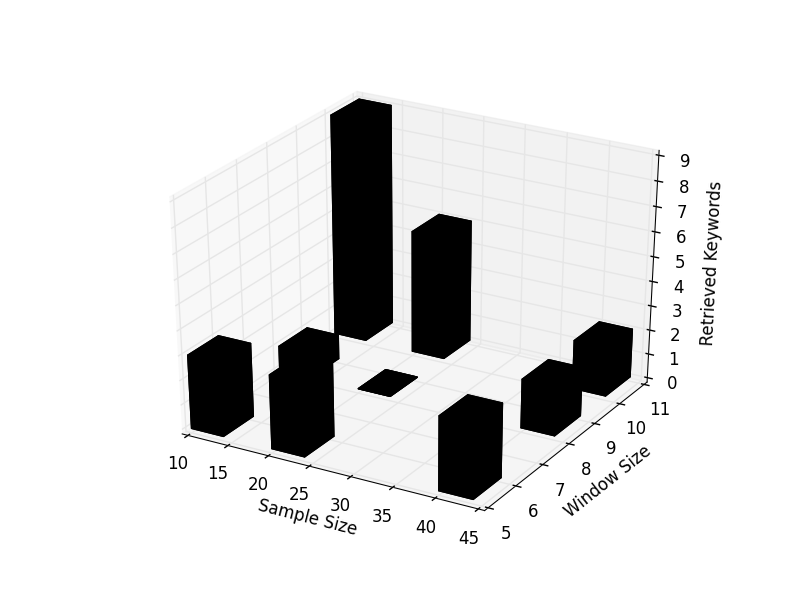
\includegraphics[width=\textwidth]{img/lex/price_hal_2}
                \caption{HAL - Price}
                \label{fig:al_price}
        \end{subfigure}%
        ~ %add desired spacing between images, e. g. ~, \quad, \qquad, \hfill etc.
          %(or a blank line to force the subfigure onto a new line)
        \begin{subfigure}[b]{0.45\textwidth}
                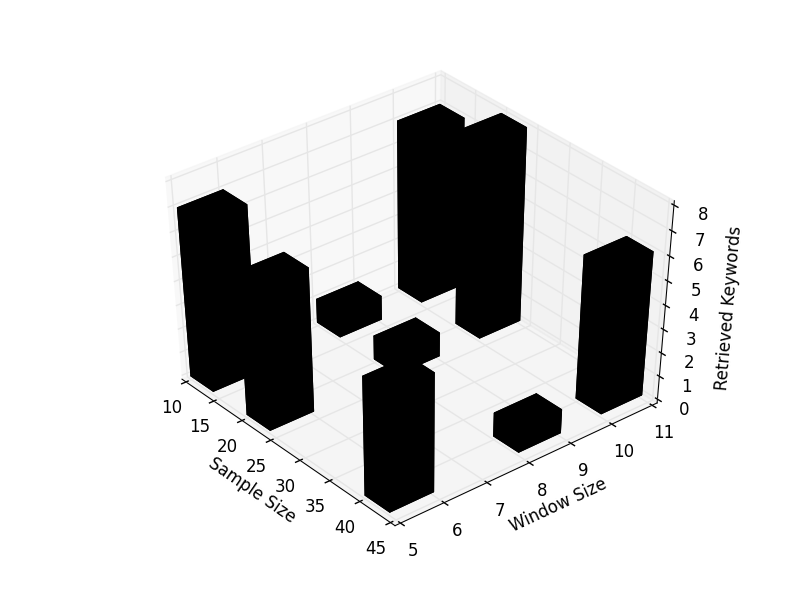
\includegraphics[width=\textwidth]{img/lex/supply_hal_2}
                \caption{HAL - Supply}
                \label{fig:hal_supply}
        \end{subfigure}
        
           \begin{subfigure}[b]{0.45\textwidth}
                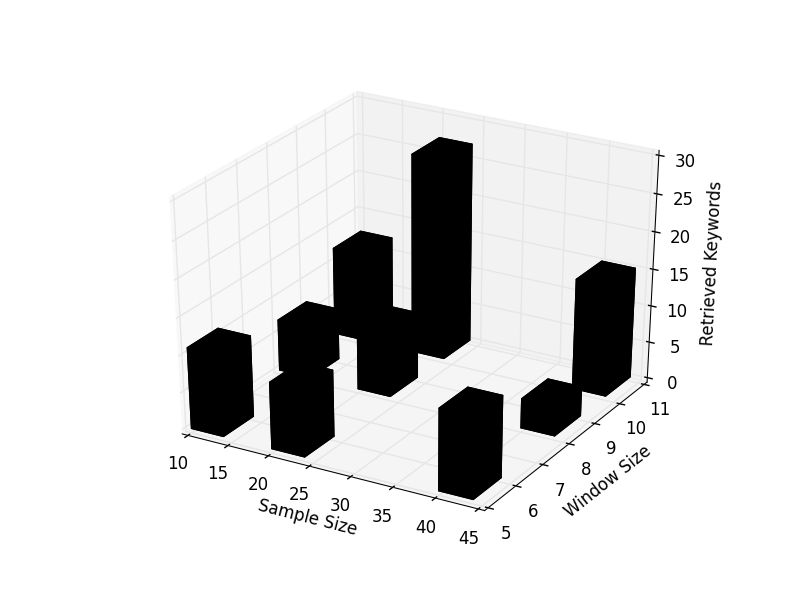
\includegraphics[width=\textwidth]{img/lex/needs_hal_2}
                \caption{HAL - Needs}
                \label{fig:al_price}
        \end{subfigure}%
        ~ %add desired spacing between images, e. g. ~, \quad, \qquad, \hfill etc.
          %(or a blank line to force the subfigure onto a new line)
       \begin{subfigure}[b]{0.45\textwidth}
                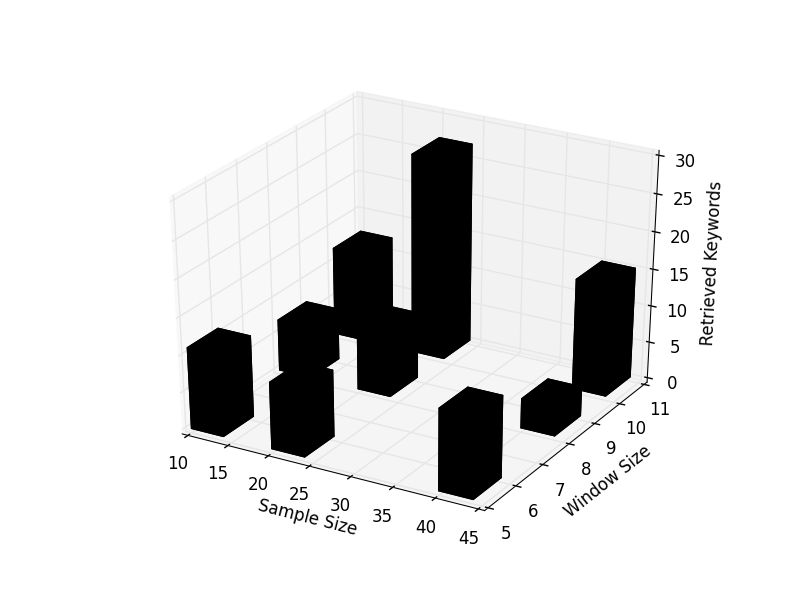
\includegraphics[width=\textwidth]{img/lex/needs_hal_2}
                \caption{HAL - Poverty}
                \label{fig:al_price}
        \end{subfigure}%
        ~ %add desired spacing between images, e. g. ~, \quad, \qquad, \hfill etc.
          %(or a blank line to force the subfigure onto a new line)

        \caption{HAL Evaluation}\label{fig:price_supply}
\end{figure}




\begin{table}[h]   
\centering
\scriptsize 
\begin{tabular}{p{1.3cm}|p{10.7cm} rlr}\toprule
\pbox{1.3cm}{Lexicon / \\ Subset $s$\\} & Keywords ( h: from HAL space, t: from thesaurus )  \\
\hline

& & \\
\pbox{1.3cm}{$Food$ \\ Supply }  & \pbox{10.7cm}{  \emph{supply}, item (h), stock (h), vendors (h), demand (h), provided (h), feeds (h), delivery (h), supply (h), industry (h), production (h), waste (h), source (h), stash (h), numbers (h), list (h), growing (h), stores (h), distribution (h), delivered (h), policy (h), purchases (h), market (h), processing (h), chain (h), packaging (h), network(h), mart (h), stalls (h), sustainability (h), aplenty (t), bags (t), bulk (t), bundle (t), chunk (t), expanse (t), extent (t), flock (t), chunk (t), gob (t), heap (t), hunk (t), jillion (v), load (t), lot (t), magnitude (t), mass (t), meassure (t), mess (t), mint (t), mucho (t), oodles (t), pack (t), pile (t), scads (t), score (t), slat (t), slew (t), ton (t), volume (t) }  \\
 & & \\
\hline
& & \\
\pbox{1.3cm}{$Food $ \\Price }  & \pbox{10.7cm}{
\emph{price}, affordable (h), cost (h), rise (h), savings (h), coupons (h), prices (h), label (h), purchase (h), economy (h), discount (h), budget (h), sales (h), benefit (h), target (h), bonus (h), size (h), money (h), better (h), best (h), free (h), buy (h), amount (t), bill (t), , demand (t), estimate (t), expenditure (t), expense (t), fare (t), fee (t), figure (t), output (t), pay (t), payment (t), premium (t), rate (t), return (t), tariff (t), valuation (t), worth (t), appraisal (t) } \\
& & \\
\hline
& & \\
\pbox{1.3cm}{$Food $ \\Poverty }  & \pbox{10.7cm}{\emph{poverty},  appetite (h), rich (h), shelter (h), homeless (h), shortage (h), control (h), provide (h), feed (h), needy (h), edible (h), nutrition (h), donate (h), 
expensive (h), economy (h), thought (h), budget (h), poor (h), service (h), supplies (h), crisis (h), demand (h), poverty (h), pantry (h), cravings (h),
 agricultural, resources, assistance, insecurity, storage (h), issue (h), bank (h), safety (h), prices (h), funding (h), health (h), drug (h), challenges (h), distribution (h), helping (h), government (h), affected (h), scraps (h), fair (h), children (h), support (h), waste (h), program (h), crops (h), restrictions (h), parcels (h), industry (h), healthcare (h), culture (h), catering (h), delicious (h), writer (h), sustainability (h), revolution (h),inflation (h), policy (h), daily (h), bankruptcy (t), debt (t), deficit (t), difficulty (t), famine (t), hardship (t), lack (t), scarcity (t), shortage (t), starvation (t),underdevelopment (t),
abundance (t), affluence (t), bounty (t), myriad (t),plenty (t), plethora (t), profusion (t), prosperity (t), riches (t), wealth (t)
  }  \\
& & \\
\hline
& & \\
\pbox{1.3cm}{$Food $ \\Needs }  & \pbox{10.7cm}{ 
\emph{need}, must (h), loving (h), share (h), like (h), favourite (h), hate (h), ordering (h), eat (h), give (h), much (h), want (h), needs (h), takes (h), beg (h), iwant (h), getting (h), favorite (h), buy (h), 50thingsilove (h), enough (h), ilove (h), whatilovethemost (h), got (h), horrible (h), cookout (h), poor (h), ate (h), deliver (h), neeeeed (h), looooove (h), neeed (h), neeeed (h), make (h), good (h), 2thingsilove (h), lack, tweetyourweakness, terrible, bring, ineed, lots (h), waiting (h), bit (h), starving (h), gave (h), delicious (h), drink (h), nice (h), cook (h), hungry (h), craving (h), healthy (h), wish (h), awesome (h), really (h), best (h), dearth (t), deficiency (t), drought (t), inadequacy (t), insufficiency (t), lack (t), need (t), omission (t), privation (t), unavailability (t), void (t), want (t),affluence (t), bounty (t), myriad (t), plenty (t), plethora (t), profusion (t), prosperity (t), riches (t), wealth (t), ampleness (t), copiousness (t), fortune (t), oppluence (t), plentitude (t), prosperousness (t)   }  \\
& & \\

\bottomrule

\end{tabular}
\caption{ Keywords of Predictor Categories}
\label{tab:pred_lex}
\end{table}
 
 \newpage
 

\section{Filtering}

The filtering of the Tweets was performed in three rounds. First we filtered for relevant food Tweets. In a second round, we applied our predictor lexicon on the retrieved set of Tweets obtained in the first step. Lastly, we filter by sentiment. The first two filtering steps are illustrated in Figure \ref{fig:lex_arch} and are labeled as \emph{Filter and Advanced Filter} respectively. 

\subsection{Food Related Tweets} 

The food related Tweets were retrieved through exact term matching, i.e. a tweet containing the term \emph{foods} would not match on the keyword \emph {food} where the reverse is also true. We mimic the term matching Twitter performs. In the initial round we optimized for coverage and hence avoided further filtering steps.The result was a collection of 29 M Tweets posted by 4.2 M users. 

\subsection{Predictor Related Tweets}

The first round  drastically reduced our dataset to around 90 GB of Tweets. With a smaller dataset we were able to perform a more involved filtering mechanism similar to \cite{hum14}. 

For every word in a tweet and every word in our predictor lexicon the stem was computed. This was necessary to capture Tweets that may contain a predictor term that is not in its base form. For example, a Tweet containing the word \emph{pricey} would not match the term \emph{price}. Furthermore the framework also accounts for miss spelt words. To do this efficiently the algorithm computes the edit distance between a given word and terms from the predictor lexicon. We return the  predictor term with the minimal edit distance if the error is in a fixed threshold 

\subsection{Sentiment Extraction}

Experiments in \cite{hum14} showed that sentiment analysers such as SentiStrength \cite{sent10} or Stanford CoreNLP \cite{stanford2011} performed  poorly on microblog content. Hence in \cite{hum14} the decision was made to extract the sentiment by having specific terms for each sentiment (polarity). Besides one had to account for changes in polarity through negations such as \emph{never} and \emph{not} which inverted the polarity of a predictor category term. 

We choose to deviate from this approach and use a sentiment analyser despite the bad results. We give two reasons for doing so. \textbf{1.)} Hutto et. al recently published a new sentiment analyser VADER \cite{hutton14} with an F1 Classification Accuracy = 0.96 which outperformed human evaluators. \textbf{2.)} Often keywords can not be manually assigned to a polarity without knowing its context. 

Besides the above-mentioned benefits \say{VADER allows us to obtain a degree of sentiment by analysing grammatical and syntactical conventions that humans use when expressing sentiment intensity} \cite{hutton14}. For example it accounts for emoticons which are commonly used to express a sentiment or even acronyms such as \emph{LOL, WTF}. It is further worth mentioning that VADER is an unsupervised approach and is well suited for streaming data. 


\chapter{Twitter Data Analysis}
\label{4}

In this chapter we provide a quantitative and a qualitative analysis of the retrieved Twitter data. In the former we want to emphasis the general popularity of food among the Twitter users and describe the term distribution of the different commodities. We further investigate if and to what extent social media data can be found to correlate with the international Food Price Index (FPI) and the commodity price quotes. This is accomplished by analysing 29 M Tweets related to food. In the qualitative analysis we focus on examining the content of Tweets and investigate the relevance to our desired food security objectives. For this purpose we automatically detect peaks in our twitter conversations and manually investigate the cause of 352 conversation spikes. 

\begin{comment}

By drawing some basic statistics we want to emphasis the general popularity of food among the Twitter users and describe the term distribution of our different commodities. In the analysis we aim to show how food terms relate to each other and how they compare to indices which are intrinsic food security indicators (e.g. \emph {affordability and availability of food}). Lastly, we investigate to what extent food security and market fundamentals are present in social media discussion. 

\end{comment}

\section{Quantitative Analysis}

To facilitate the comprehension of our Twitter dataset we draw some basic statistics of the user and term distribution. The later illustrates the volume increase that we achieved through iteratively improving our lexicon in Section \ref{food_lex}. Lastly we perform a through correlation analysis between food conversations and the FPI. 

\subsection {User Distribution}

Twitter is a social network and in general such networks follow a power law distribution \cite{Whittaker:1998}. We see in the below Figure \textbf{\ref{fig:user_1}} and Figure \textbf{\ref{fig:user_2}}  that the distribution of the number of Tweets per user deviates from a normal power law. A lot of individuals  send only a few Tweets about the subject and only a small number of users transmit a large amount of Tweets. Unlike \cite{bild15} suggest the contribution participation level of  80 \%, 20 \%   does not seem to apply to Tweets about food. In Figure \ref{fig:no_power} we can see that the curve is almost linear. About 50 \% of the Tweets are caused by 50 \% of the users. This deviates highly form the normally observed 80 \%, 20 \% ratio. We assume that this is due to the wide spread interest of the topic.




\begin{figure}
        \centering
        \begin{subfigure}[b]{0.5\textwidth}
                \includegraphics[width=\textwidth]{img/anal/loglog_users_Tweets_1}
                \caption{LogLog: Number of Tweets per User}
                 \label{fig:user_1}
        \end{subfigure}%
        ~ %add desired spacing between images, e. g. ~, \quad, \qquad, \hfill etc.
          %(or a blank line to force the subfigure onto a new line)
        \begin{subfigure}[b]{0.5\textwidth}
                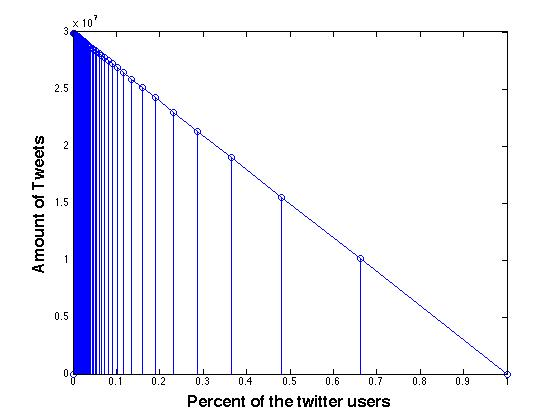
\includegraphics[width=\textwidth]{img/anal/no_power_1}
                \caption{Distribution: Number of Tweets per User}
                \label{fig:user_2}
        \end{subfigure}
        ~ %add desired spacing between images, e. g. ~, \quad, \qquad, \hfill etc.
          %(or a blank line to force the subfigure onto a new line)
      
        \caption{User Distribution}\label{fig:animals}
\end{figure}





\subsection {Food Term Distribution}

Our framework for the data acquisition successfully increased the total volume of food related Tweets. From an initial 13.7 M Tweets we raised the entire volume by 110\% to a total of 29.9 M food related Tweets. The distribution of the volume per food term is displayed in Figure \ref{fig:world}. We illustrate in light grey the added volume alongside the initial size in dark grey. The most popular food terms on Twitter are general terms such as \emph{food, dinner and lunch}. Within the 10 most popular terms we found that three beverages (coffee, beer, tea) were represented. The most popular traded commodity term on social media is chicken.  We further show the distribution of the categories in \ref{fig:cat}. By far the highest contribution has the category \emph{other food of interest} due to general food related keywords such as \emph{dinner} or \emph{food}. It builds the absolute majority with 51 \%. Meat related keywords have the second highest contribution with around 15 \% followed by 12\% sugar, 11\%  cereals, 10 \% dairy  and lastly 0.2 \% vegetable oils. We would like to note that the volume roughly follows the economic importance of the different categories with the only outlier being sugar \cite{fao2008}. We assume this is due to the highly popular products \emph{coca cola} and {chocolate} which caused alone 70 \% of the sugar related Tweets. 



\begin{figure}[H]
        \centering
        \begin{subfigure}[b]{0.5\textwidth}
                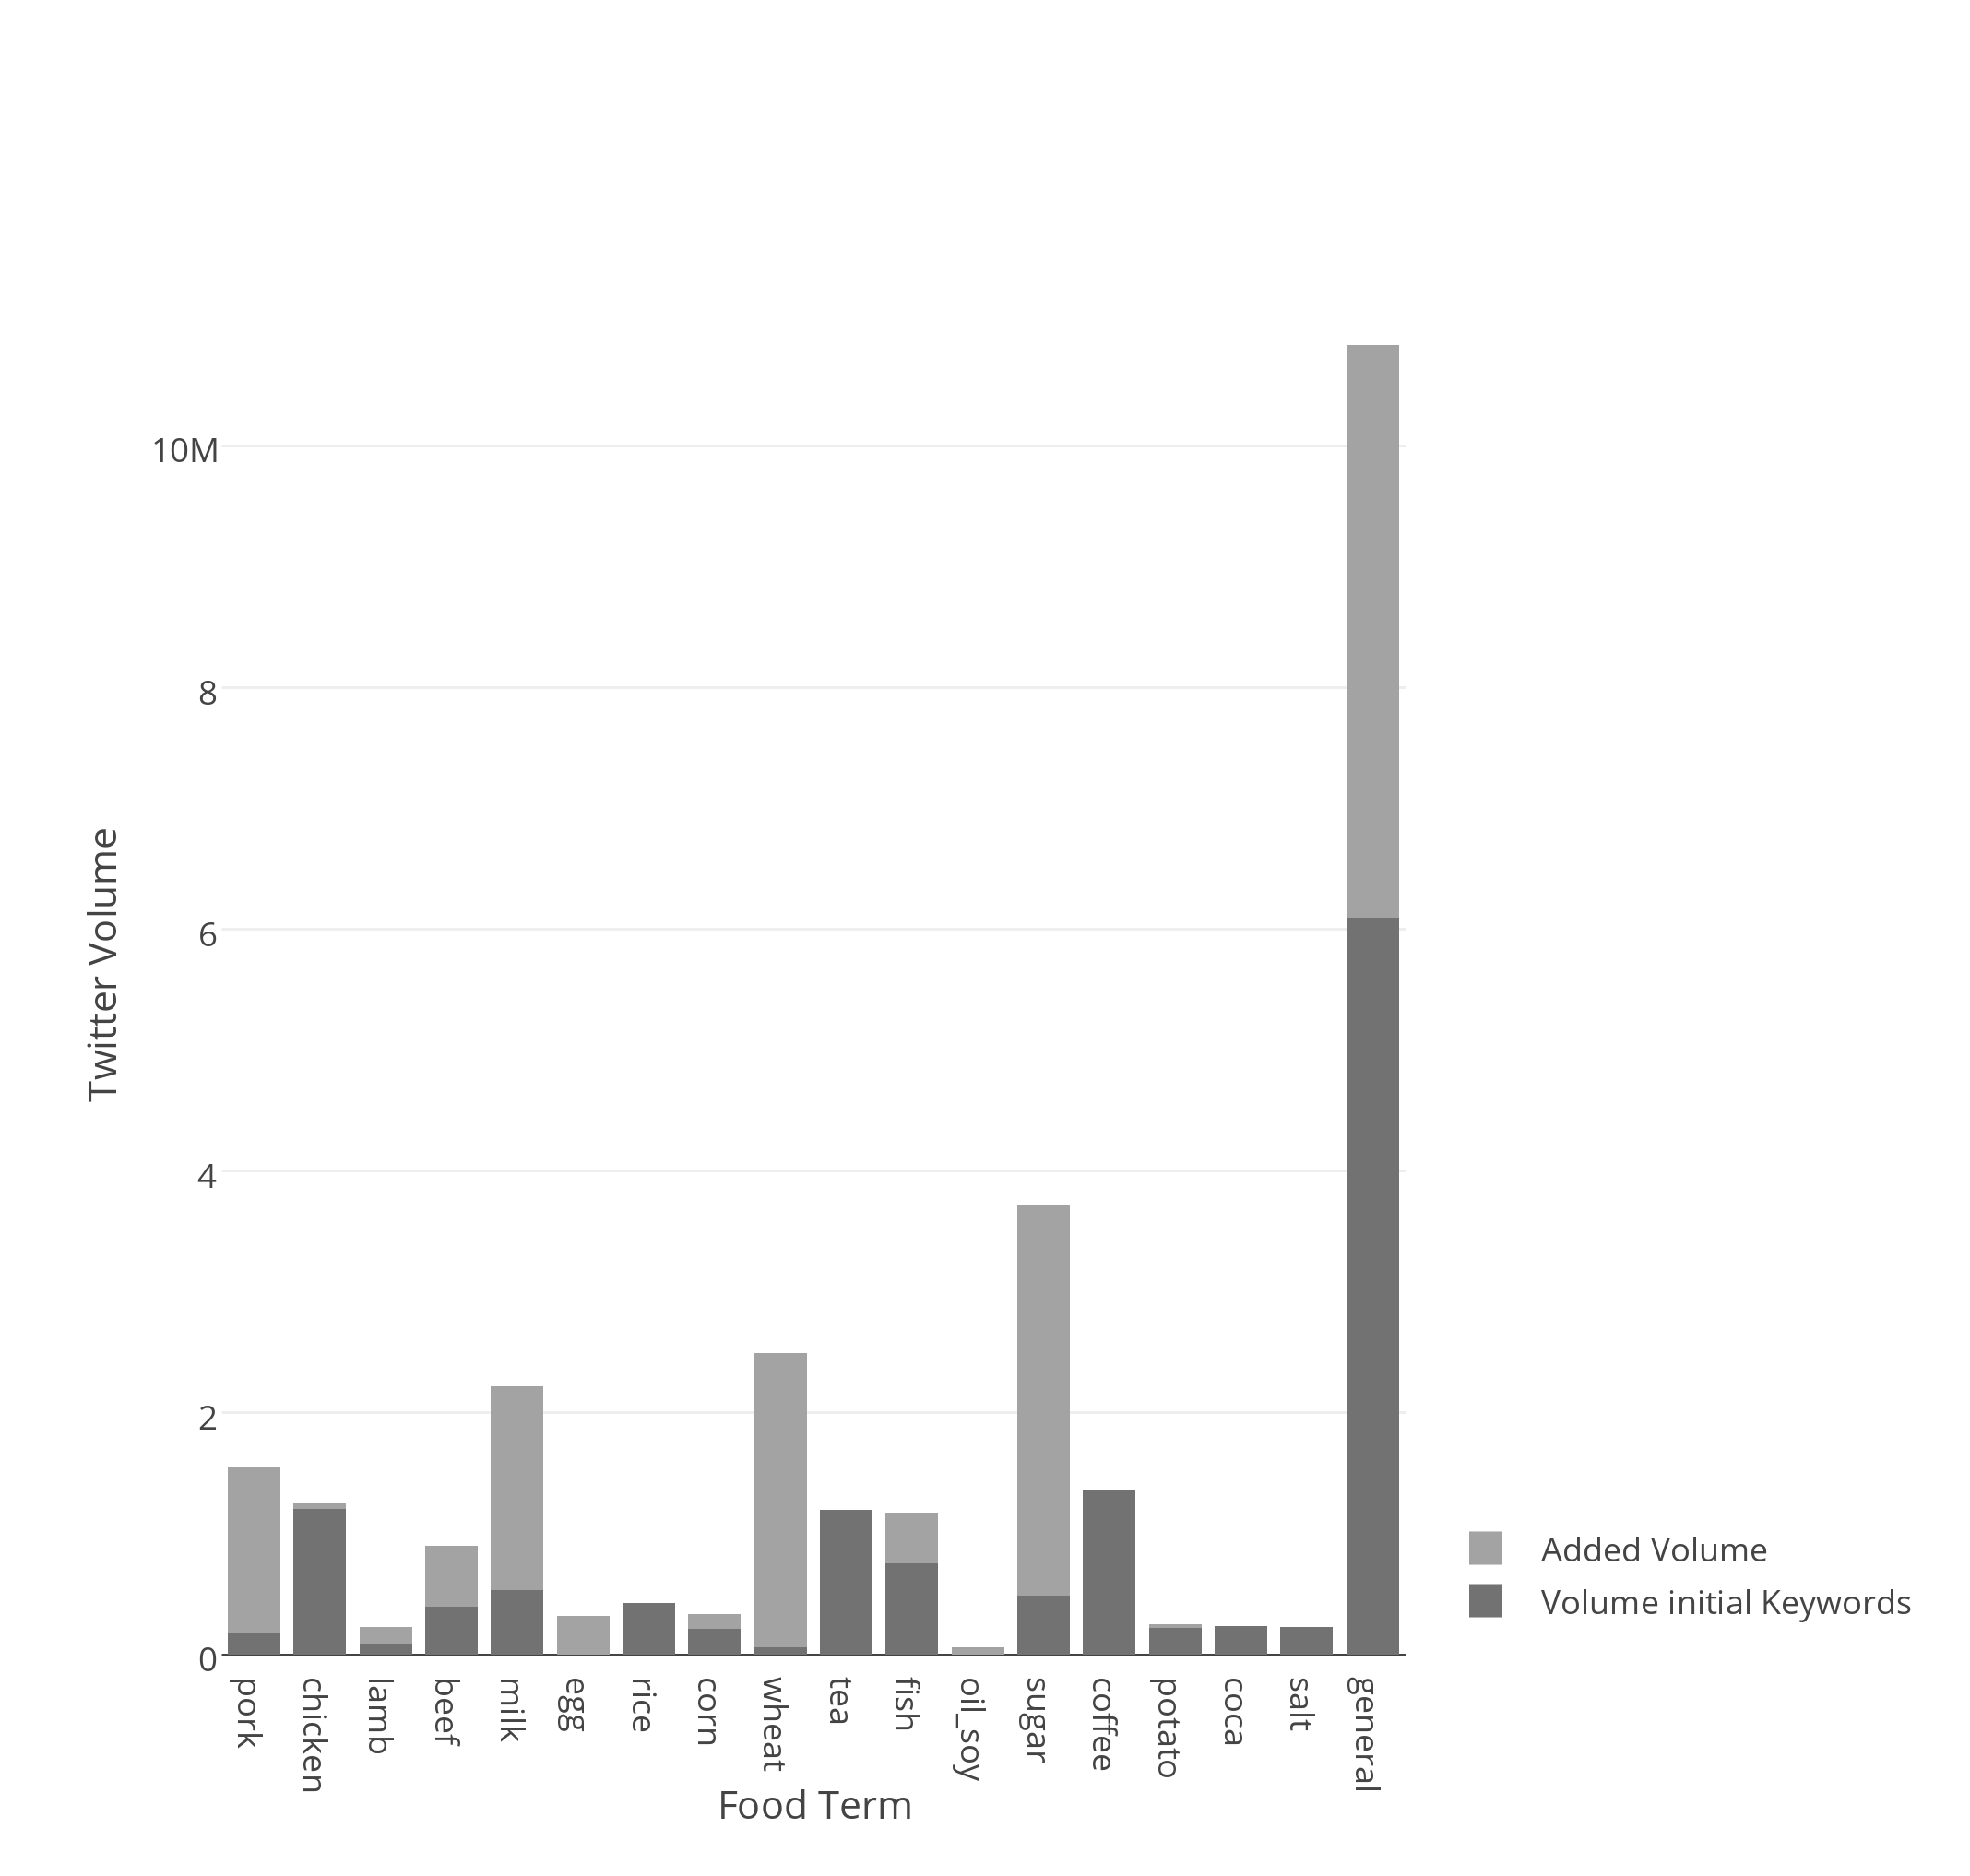
\includegraphics[width=\textwidth]{img/anal/exp_dist_1}
                \caption{Overall Distribution}
                \label{fig:world}
        \end{subfigure}%
        ~ %add desired spacing between images, e. g. ~, \quad, \qquad, \hfill etc.
          %(or a blank line to force the subfigure onto a new line)
        \begin{subfigure}[b]{0.5\textwidth}
                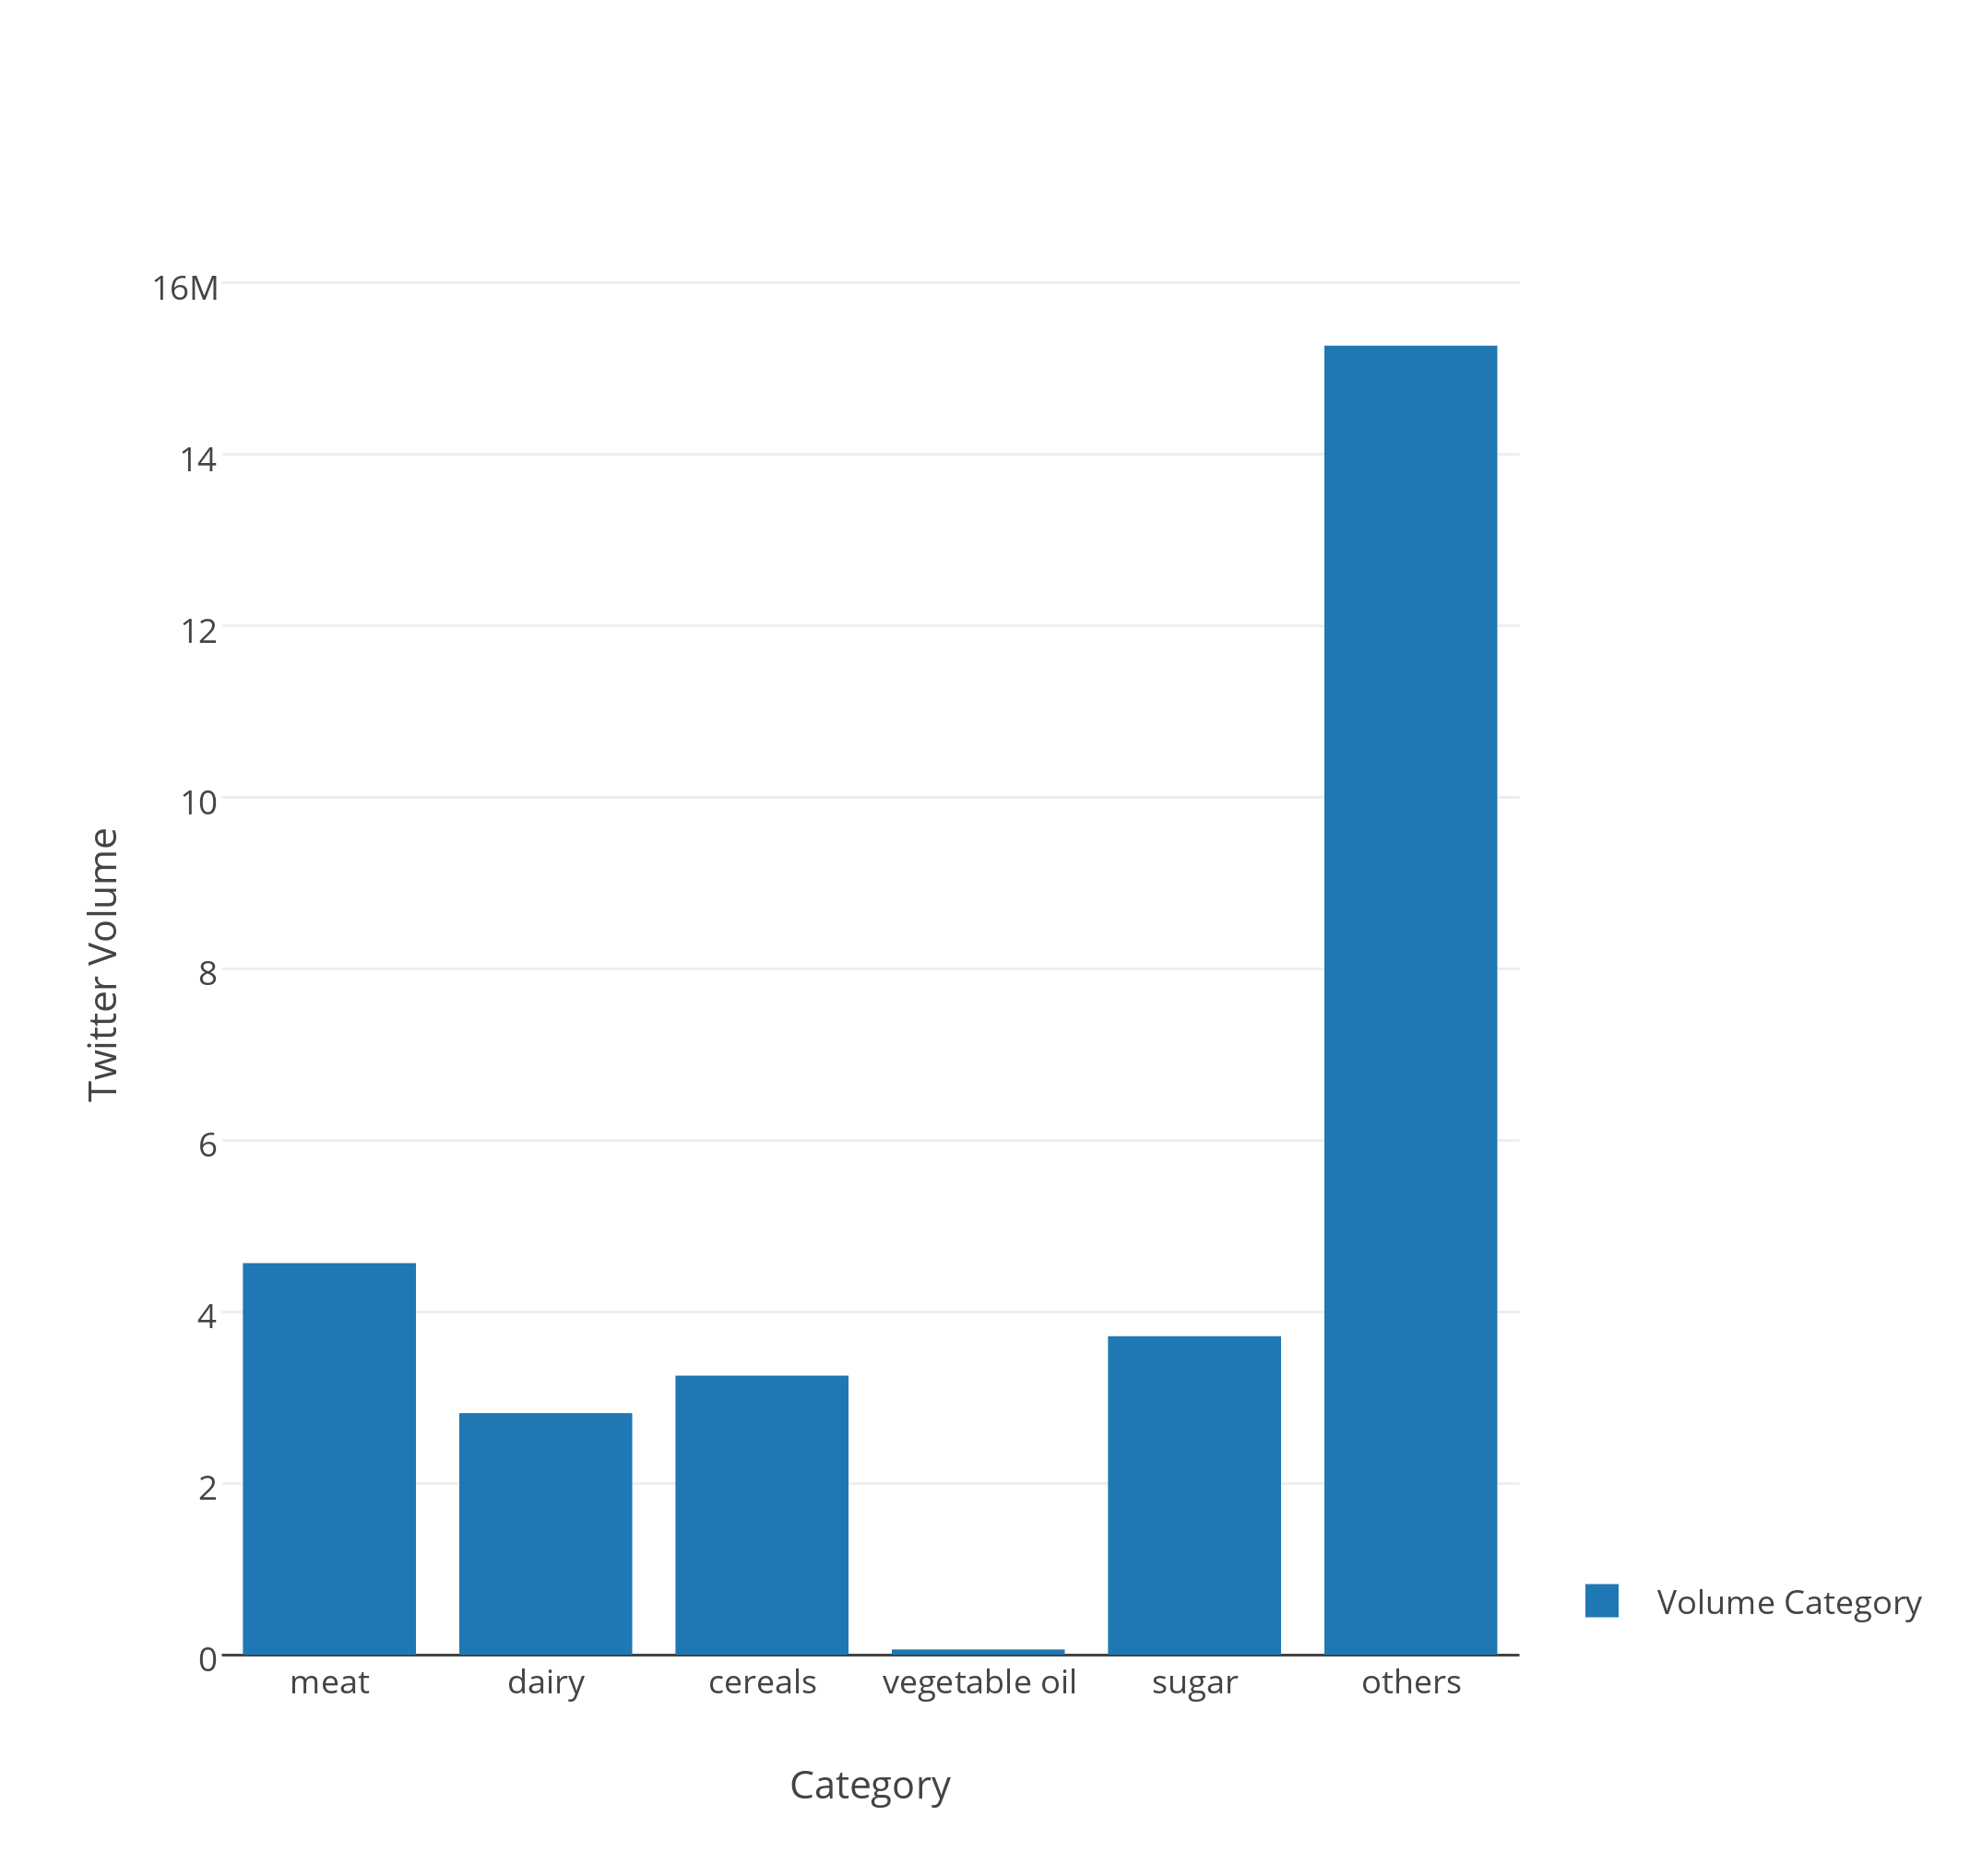
\includegraphics[width=\textwidth]{img/anal/exp_dist_cat_1}
                \caption{Category Distribution}
                \label{fig:cat}
        \end{subfigure}
        ~ %add desired spacing between images, e. g. ~, \quad, \qquad, \hfill etc.
          %(or a blank line to force the subfigure onto a new line)
      
        \caption{Volume of Tweets per Keyword and per Category}\label{fig:distribution}
\end{figure}


\subsection{Price Correlation}
\label{corr}

%The weighted average of those five categories as illustrated in \cite{fao13}  defines the international food price index which is an overall measure of the current food condition. 

We observed a general popularity of food in our initial analysis and that certain food categories have a much stronger presence than others. There is however still a concern on whether the sampled data is useful to detect difference in price fluctuation and lastly can  be used as medium to determine food security. For the purpose of this correlation analysis we used the price quotations of the Food and Argriculture Organisation of the United Nations \footnote{http://www.fao.org/worldfoodsituation/foodpricesindex/en/} and commodity quotes from candle \footnote{https://www.quandl.com/}. FAO differentiates between a Category Food Price Index (CFPI) and a universal FPI. The CFPI is specific to a food category (e.g. meat, cereals) so different among all categories, whereas the FPI is a general indicator and  the same for all categories. Unfortunately daily commodity quotes could only be obtained for meat, dairy and cereals. 

For each food category (e.g. \emph{meat, dairy} ) we correlated the tweet volumes of the subcategories( e.g. \emph{beef, chicken for meat}), products (e.g. \emph{bacon, salami}) and the price quotes for each category. These subcategories mirror the categorisation of the FAO \cite{fao2008}. Since the price quotes of the FAO are based on a monthly average, we aggregated the daily tweet volumes per food term over a month and calculated the daily average volume. We only included food terms that have an average of greater than 10 Tweets per day. The internet archive did not contain Tweets for certain days. We approximated those values by taking the average of the previous and the following day. 

\subsubsection{Results} 
\label{corr_results}

Between the meat subcategories there is a  positive linear relationship in the range of 0.7264 to 0.9361.This means if the volume of chicken Tweets increases so do the volumes of beef and pork conversations. A $p$ value of 0.0001 suggest that we can reject the idea that the correlation is due to random sampling. No clear relationship exists between the tweet volume of the meat category and the three price indices. A slight correlation for the meat subcategories was observed where all of them were negatively correlated to the price quotes meaning that if the volume increases the price will most likely decrease. Only a few sub products showed a significant correlation with the price quotes. A positive relationship can be seen between the term goat and the commodity price with a correlation of 0.7369 and a p value of 0.0001. A possible explanation might be its popularity among developing countries. 95\% of the world's 475 million goats are located in developing countries \footnote{http://www.fao.org/docrep/009/ah221e/AH221E13.htm}. People consuming goat meat would be more sensitive towards price fluctuation making it potentially a valuable feature in measuring food prices. By correlating the price indices we see that there is a strong positive relationship between the FAO meat price index and the commodity quotes. This analysis supports Abbott et al's theory \cite{abbott2009}  that the commodity markets have a strong influence on the rising food prices and are a strong indicator for measuring food security. 



\begin{figure}[H]
        \centering
         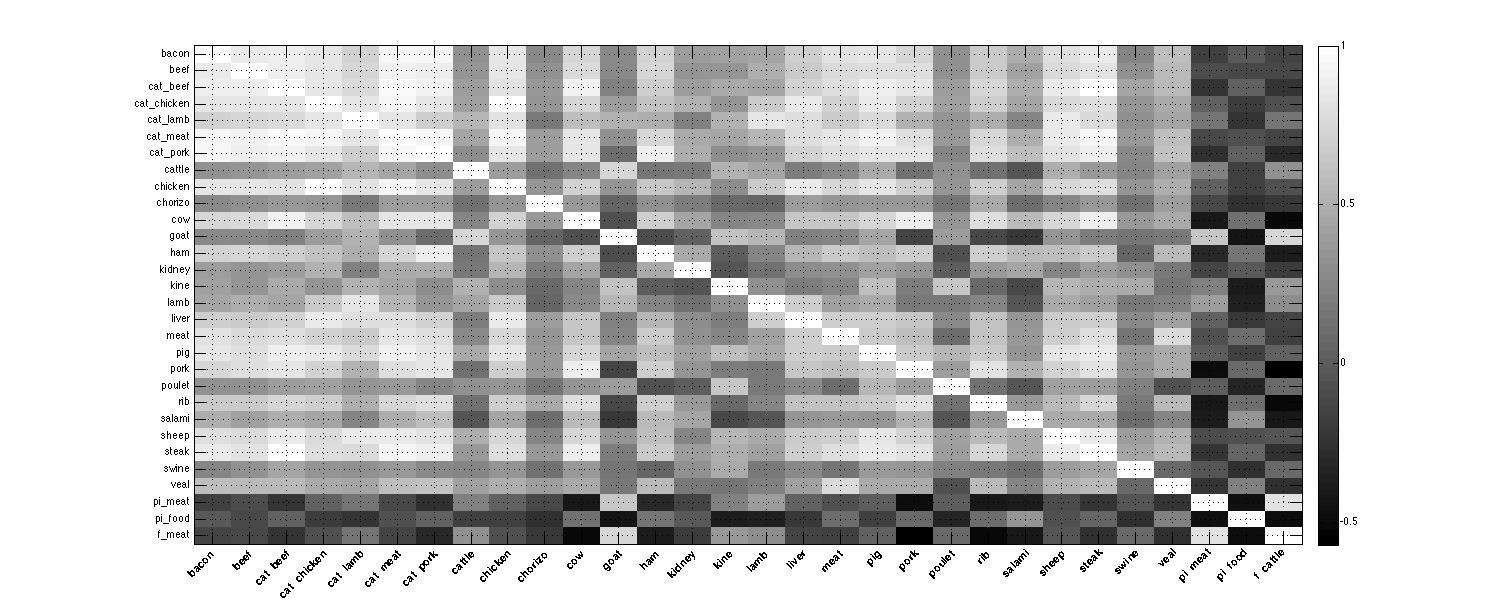
\includegraphics[width=1\textwidth ]{img/anal/meat_black}
              
        \caption{Heatplot Meat: Volume of Tweets per Keyword and per Category}
        \label{fig:distribution}
\end{figure}



For cereals similar to meat we likewise see a high correlation in volume of around 0.82 between the different cereal categories. The products \emph{beer, barley, bread, atta and pasta} show a strong positive relationship to the cereal categories. Unlike meat, the cereal category price index and the commodity price show a strong positive relationship with the universal FPI. This is somewhat surprising as meat prices have a stronger influence on the universal FPI then cereals do \cite{fao2008}. Furthermore the product pasta has a strong linear relationship with the commodity price of 0.7212.
\begin{figure}[H]
        \centering
         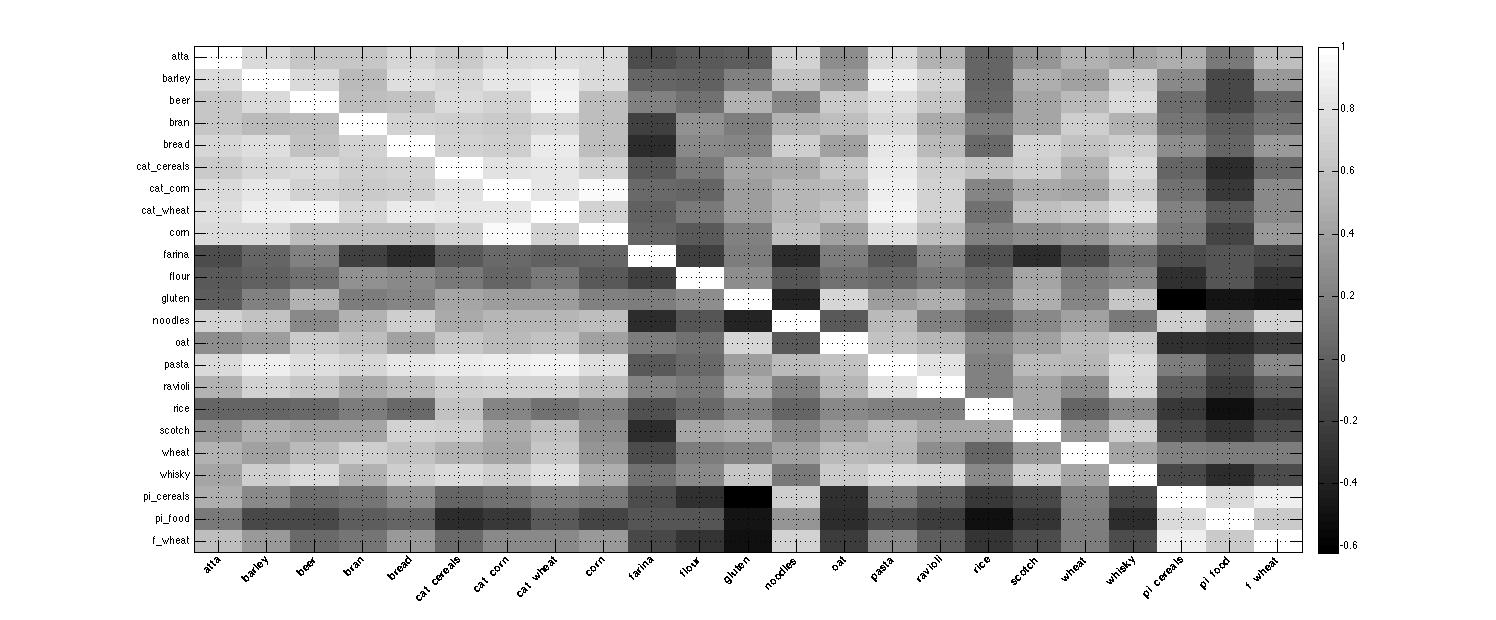
\includegraphics[width=1\textwidth ]{img/anal/black_cereals}
              
        \caption{Heatplot Cereals: Volume of Tweets per Keyword and per Category}
        \label{fig:distribution}
\end{figure}
 

The heat plots of dairy, sugar and oil show yet again no clear linear relationship between the Twitter volume and the food price indices. More so than in other food categories the subcategories of dairy can be clearly distinguished through its strong correlation with the different products (i.e. mozzarella has a strong relationship with the category cheese and only a weak correlation with milk products). The heat plot for dairy, sugar and oil have been added to the appendix \ref{pCorr}.



\subsubsection{Discussion} 

Our analysis did not show a significant correlation between the raw attention on food and the price quotes.
Nonetheless the insights gained from this analysis will help us improve our features. For example the category meat shows a number of products that have a strong negative correlations. By only including such terms we are hoping to strengthen the relationship between the meat category and the price quotes.

 Although we can not provide any scientific evidence there might be a nonlinear relationship between social media and the commodity market. We hence will experiment with a non-linear model to predict price quotes in Chapter \ref{model}. According to \cite{de08} such models are better suited to utilise social media for predictions. 

A smilier correlation analysis has been made by the UN \cite{ungp2013}. They however used contextual sensitive Tweets i.e. instead of only using Tweets containing food they performed an n-match on different criteria. The tweet had to contain a food item, the word price and a quantification such as high or low. Overall a Pearson correlation of around 0.42 was detected with a significance of 0.04. By exploiting our predictor lexicon to filter Tweets that contain keywords such as supply and price we were able to improve the linear relationship and found similar results as in \cite{ungp2013}. Although the UN concluded a linear relationship they simply provided assumptions about what might have caused the volatility of price conversations. We hence explore the conversation drivers in the next section. 
 

 
\begin{table}[h]   
 \begin{tabular}{  c  | c  | c | c }
			
   & \textbf{Category Price Index}  & \textbf{Food Price Index} & \textbf{Commodity Price Index} \\
  \hline 
  &&& \\
  Meat & -0.0112   & -0.0653 & - 0.1489  \\
  
  Dairy & -0.2166   & 0.1314 & -0.0676\\

  Cereals & 0.0357  & -0.3360 & 0.0594 \\

  Oil & -0.2484  &  -0.2382 & -   \\

  Sugar & -0.2000 & -0.1019 &  - \\

\hline 

\multicolumn{3}{c}{\null}\\

\multicolumn{3}{c}{\textbf{Significance:} p $<$ .0005 ***, p $<$ 0.005 **, p $<$ 0.05 *}\\
\hline  

\end{tabular}
\caption{Price Correlation}
\label{tab:abc}


\end{table}


 \section{Qualitative Analysis of Conversation Drivers}
 \label{conversation}


Following our quantitative analysis we proceed with a detailed investigation of Twitter conversations relevant to food security to uncover events that trigger conversations. We found that our contextual sensitive Tweets (i.e. such tweet that contain a food term and a predictor term such as price) have a stronger Pearson correlation than the raw volume. Encouraged by this observation we want to investigate further to which extent the Tweet content is related to food security. By means of a visual analysis we first characterise the temporal behaviour of our twitter conversations an manually investigate the major peaks to verify that such spikes are caused by real life events. With the intent to automate the detection of real life events (we will interchangeably use events or spikes to refer to peaks) we introduce a methodology and introduce a semi automated approach to identify the conversation driver. Lastly, we present the annotation categories and the results of this section. 

\begin{comment}

 More specifically we want to know if the conversations can be related to market fundamentals that cause soaring food prices. Following the two recent food crises in 2007 and 2010 a lot of research has been centered around defining causes of volatile food prices.  In \cite{Tadesse2014} they define a taxonomy for drivers of  international food price spikes and differentiate among three different causes namely exogenous shocks, conditional causes and internal causes. Examples of exogenous shocks are extreme weather events, oil price shocks, economic and demand/supply growth, and lastly economic shocks. Conditional causes can originate through political conflict or market conditions. Internal causes on the other hand are speculative activities(driven by price expectations) and declines in world food stocks. This taxonomy will serve us as a baseline in annotating our events. 
\end{comment}



\subsection{A Visual Analysis of the Social Attention}

We commence our investigation of the conversation drivers by a visual and manual investigation of the most prominent spikes. To gain an overview about the social attention of our food topics we plotted the relative distribution of food supply, price poverty and needs in Figure \ref{fig:topic_dist}. By far the highest attention is attributed to food needs with around 70 \% , poverty and supply receive a similar attention distribution with price taking the smallest interest among Twitter users. 

To visually categorise the activity, Lehman et al. \cite{Lehmann2012} defined three categories of temporal behaviours. \say{Continuous activity, periodic activity or activity concentrated around an isolated peak}. Continues activities are topics that are of daily interest such as weather. On the other hand periodic actives reoccur with a fixed pattern such as the release of a popular Tv show. The latter is event driven and usually occurs once during a very short period such as a national holiday. 

For price and supply we observe a similar temporal pattern. Both show a continuous activity with one extremely prominent isolated peak. The activity is concentrated symmetrically around those two events , showing abnormal activities for around 9 days before and after. 

 We manually investigated the two isolated peaks to see if we can attribute them to any discussions relevant to food price or food supply. Surprisingly, the content in the price discussion corresponds to a popular Korean pop band \emph{T-ara }. \emph{T-ara } released a music video on the 10th of September which caused the first anomaly, reaching a global maximum on the 16th when they announced to collaborate with a famous European DJ  \footnote{http://www.kpopstarz.com/articles/112632/20140916/t-ara-sugar-free.htm}. Similarly, in our supply conversation the peak was not caused by supply indicators but was driven by conversations centered around health \& life style topics. 

The topics needs and poverty do not exhibit any extreme outliers and similar to price and supply can be categorised according to Lehman et al's. framework as of continuous interest. 




\begin{figure}[H]
        \centering
         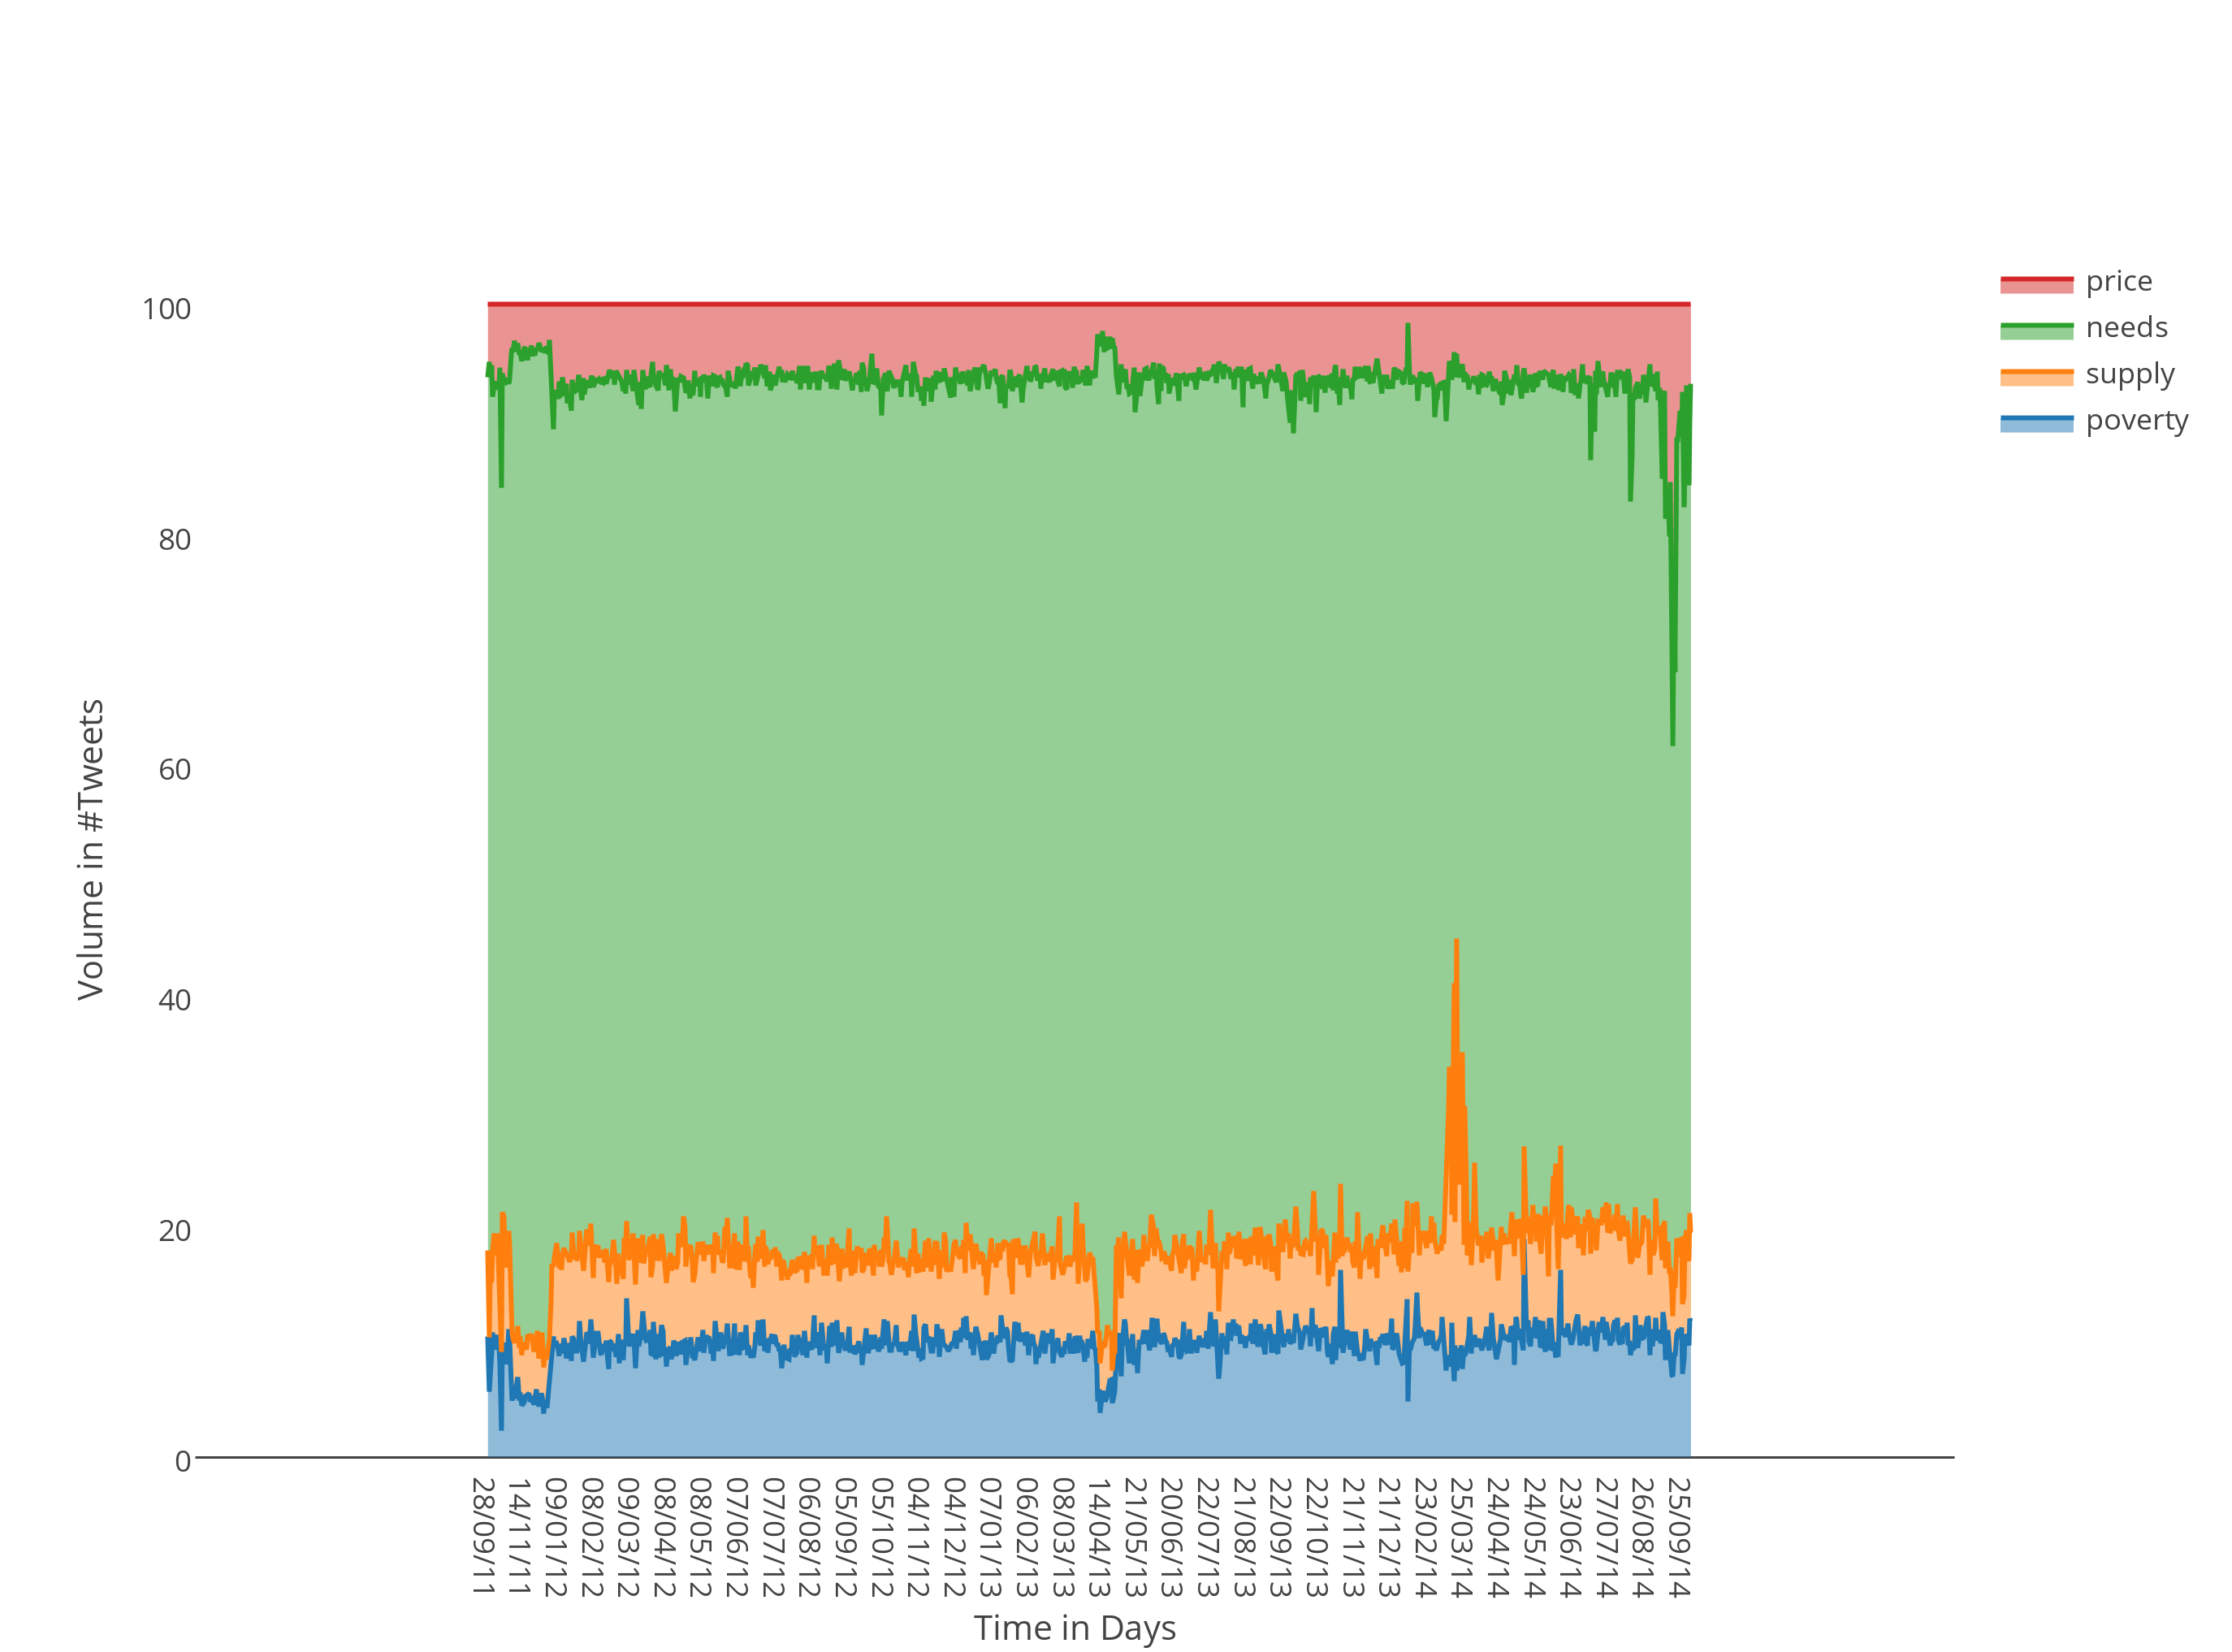
\includegraphics[width=1\textwidth ]{img/anal/topic_dist}
              
        \caption{Topic Distribution - Food Security}
        \label{fig:topic_dist}
\end{figure}




\subsection{Event Detection} 

As described in the previous section the prominent peaks could not be attributed to any discussion around indicators that are relevant to food security. To facilitate the automatic detection of peaks we now introduce an automated approach similar to\cite{olt15} \cite{Lehmann2012}. We evaluate the four food categorie's temporal behaviour on a granularity of one day. This scale was chosen in order to be in accordance with the temporal quotations of the commodity market. To detect peaks in our food topics we used a fixed window size of $2m + 1$  where $m = 15$ giving us a month long window. Within the window we identified the median and calculated the mean of the Twitter volume. From those values we calculated the Median absolute deviation (MAD) as in Equation \ref{eq:mad}: 

\begin{equation} \label{eq:mad}
\overline{ MAD } = median_i (|X_i - median_j(X_j)|)\end{equation}


$X_j$ is the set of data points within the fixed window and $X_i \in X_j$

A peak is declared if $v_i$ deviates more than 2 MAD from the mean. For this analysis we only consider positive peaks and ignore anomalies in form of a steep descent. 

The discussion centered around food price showed 82 peaks. Tweet activities for food supply resulted in 91 peaks. 80 peaks were detected for food needs and lastly 99 for food poverty. 
 

To identify what topics spike the attention we follow the approach discussed in \cite{olt15}. We computed the top 50 unigrams and top 10 bigrams of all Tweets occurring during a peak. We then manually investigate the Tweets that contain the most frequent n-grams. Some peaks could be attributed to multiple events. If two conversation drivers could be identified, both of them were used to label the peak. Else, if most likely more than two events caused the peak we marked it as ambiguous.  

\subsection{Event Annotation}

We annotate each peak according to the definitions given below. Our classification mostly mimics the main dimensions of food security but also includes categories from the taxonomy of Tadesse et al\cite{Tadesse2014}. There is a strong overlap between the two taxonomies where the later focuses more on Economic Access and the former has a stronger orientation towards Food Utilisation. This categorisation is not extensive i.e. there are a range of further categories we could consider. However given the sparsity of relevant events this classification gives a good overview of the discussed topics. 

Some events show causal relationships i.e. a breach in the food supply can be a cause for riots and political unrests. In such cases we annotated both. 


\begin{description}
  \item[Food Supply ] \hfill \\
 Events entered around the food supply chain are considered including indicators of food waste. We define Food Loss and Food waste according to Parfitt et al. 's \cite{Julian10} definition. Food Waste refers to Food Loss that occurs at the retailers and consumers side whereas the term Food Loss refers to the decrease in food volume that leads to edible food for consumption.
  \item[Economic Access] \hfill \\
  We define Economic Access according to FAO's \cite{fao2008} definition. Price, expenditure or market indicators fall into this domain.   
  \item[Government] \hfill \\
  The classification Government takes topics such as legislation and policy changes into account. An example is restrictive trade policies such as export or import restrictions  \cite{Tadesse2014}. 
    \item[Stability] \hfill \\
 Poverty,  political unrest and topics concerning extreme weather \cite{fao2008} fall into this classification. Factors that cause insecurity such as riots or severe draughts are considered. 
    \item[Unrelated] \hfill \\
   Viral jokes,  advertisements, health \& lifestyle are example topics that we consider unrelated. 



\end{description}








Our findings showed that for price only 7 (8.5 \%) out of 82 fell into the above given categories, for  supply 4 (4.3 \%) out of 91 for poverty 13 ( 13 \%) out of 99 and finally for needs no relevant topics were found. 


\subsection{Results}
\label{an_result}

The distribution of the annotations is visualised in Figure \ref{fig:annotation_dist}. Surprisingly the conversations mostly peaked outside their domain, i.e. the price conversation was more intrinsic for supply indicators then for economic access indicators. We now give examples to each annotation topic of events that we classified as food security relevant to illustrate what kind of discussion caused a peak . 



\begin{description}
  \item[Food Supply ] \hfill \\
 Topics that caught the social media audience were especially safety threats to the food supply. In April 2012 a newly discovered case of cow disease threatened the safety of America's beef supply and heavy import restrictions were imposed from major beef importers such as South Korea \footnote{http://www.theguardian.com/science/2012/apr/25/mad-cow-disease-us-mutation}.
  \item[Economic Access] \hfill \\
  In 2014 sharp rising food prices caused a lot of discussion on Twitter. Wholesale prices were suffering due to a severe drought in the previous year, which thinned the cattle herds and increased consumer prices \footnote{http://www.cnbc.com/id/101588110}. As a consequence there was also a sharp increase in discussion around food banks. The UK observed a 51 \% increase in food bank users \footnote{http://www.bbc.com/news/business-27032642}. 
  \item[Government] \hfill \\
  Most discussions around legislation changes were focused on Food Bank reforms. A high amount of attention can be attributed to the UK rejecting the European Union food bank funding. The population heavily criticised the British government to deny EU fund to be spent on the poor \footnote{http://www.theguardian.com/society/2013/dec/17/government-under-fire-eu-funding-food-banks}
    \item[Stability] \hfill \\
  Discussions around stability were usually headlined by extreme poverty causing riots. A food program that provided free lunch to underprivileged school kids used poisoned crops in their dishes. 20 children died as a consequence causing riots and closed shops all over the city. \footnote{http://www.usatoday.com/story/news/world/2013/07/17/india-children-deaths/2523727/}
   \item[Unrelated] \hfill \\
   Unrelated topics cover a vast amount of domains. Most often peaks are caused by viral Tweets posted by online celebrities that contain a food term. Public holidays, such as Easter, Thanks Giving are also frequently captured. Furthermore public figures such as Ray Rice, a famous football player, caused a lot of hype in the social media community \footnote{http://www.nytimes.com/2014/09/09/sports/football/ray-rice-video-shows-punch-and-raises-new-questions-for-nfl.html}. Often it was very hard to extract the conversation drivers in the unrelated topics. There is a considerable amount of noise in our conversations centered around food security, making it very challenging to extrapolate meaning from an event. This might be attributed to the general popularity of food we identified in previous chapters. 

\end{description}




\begin{figure}[H]
        \centering
         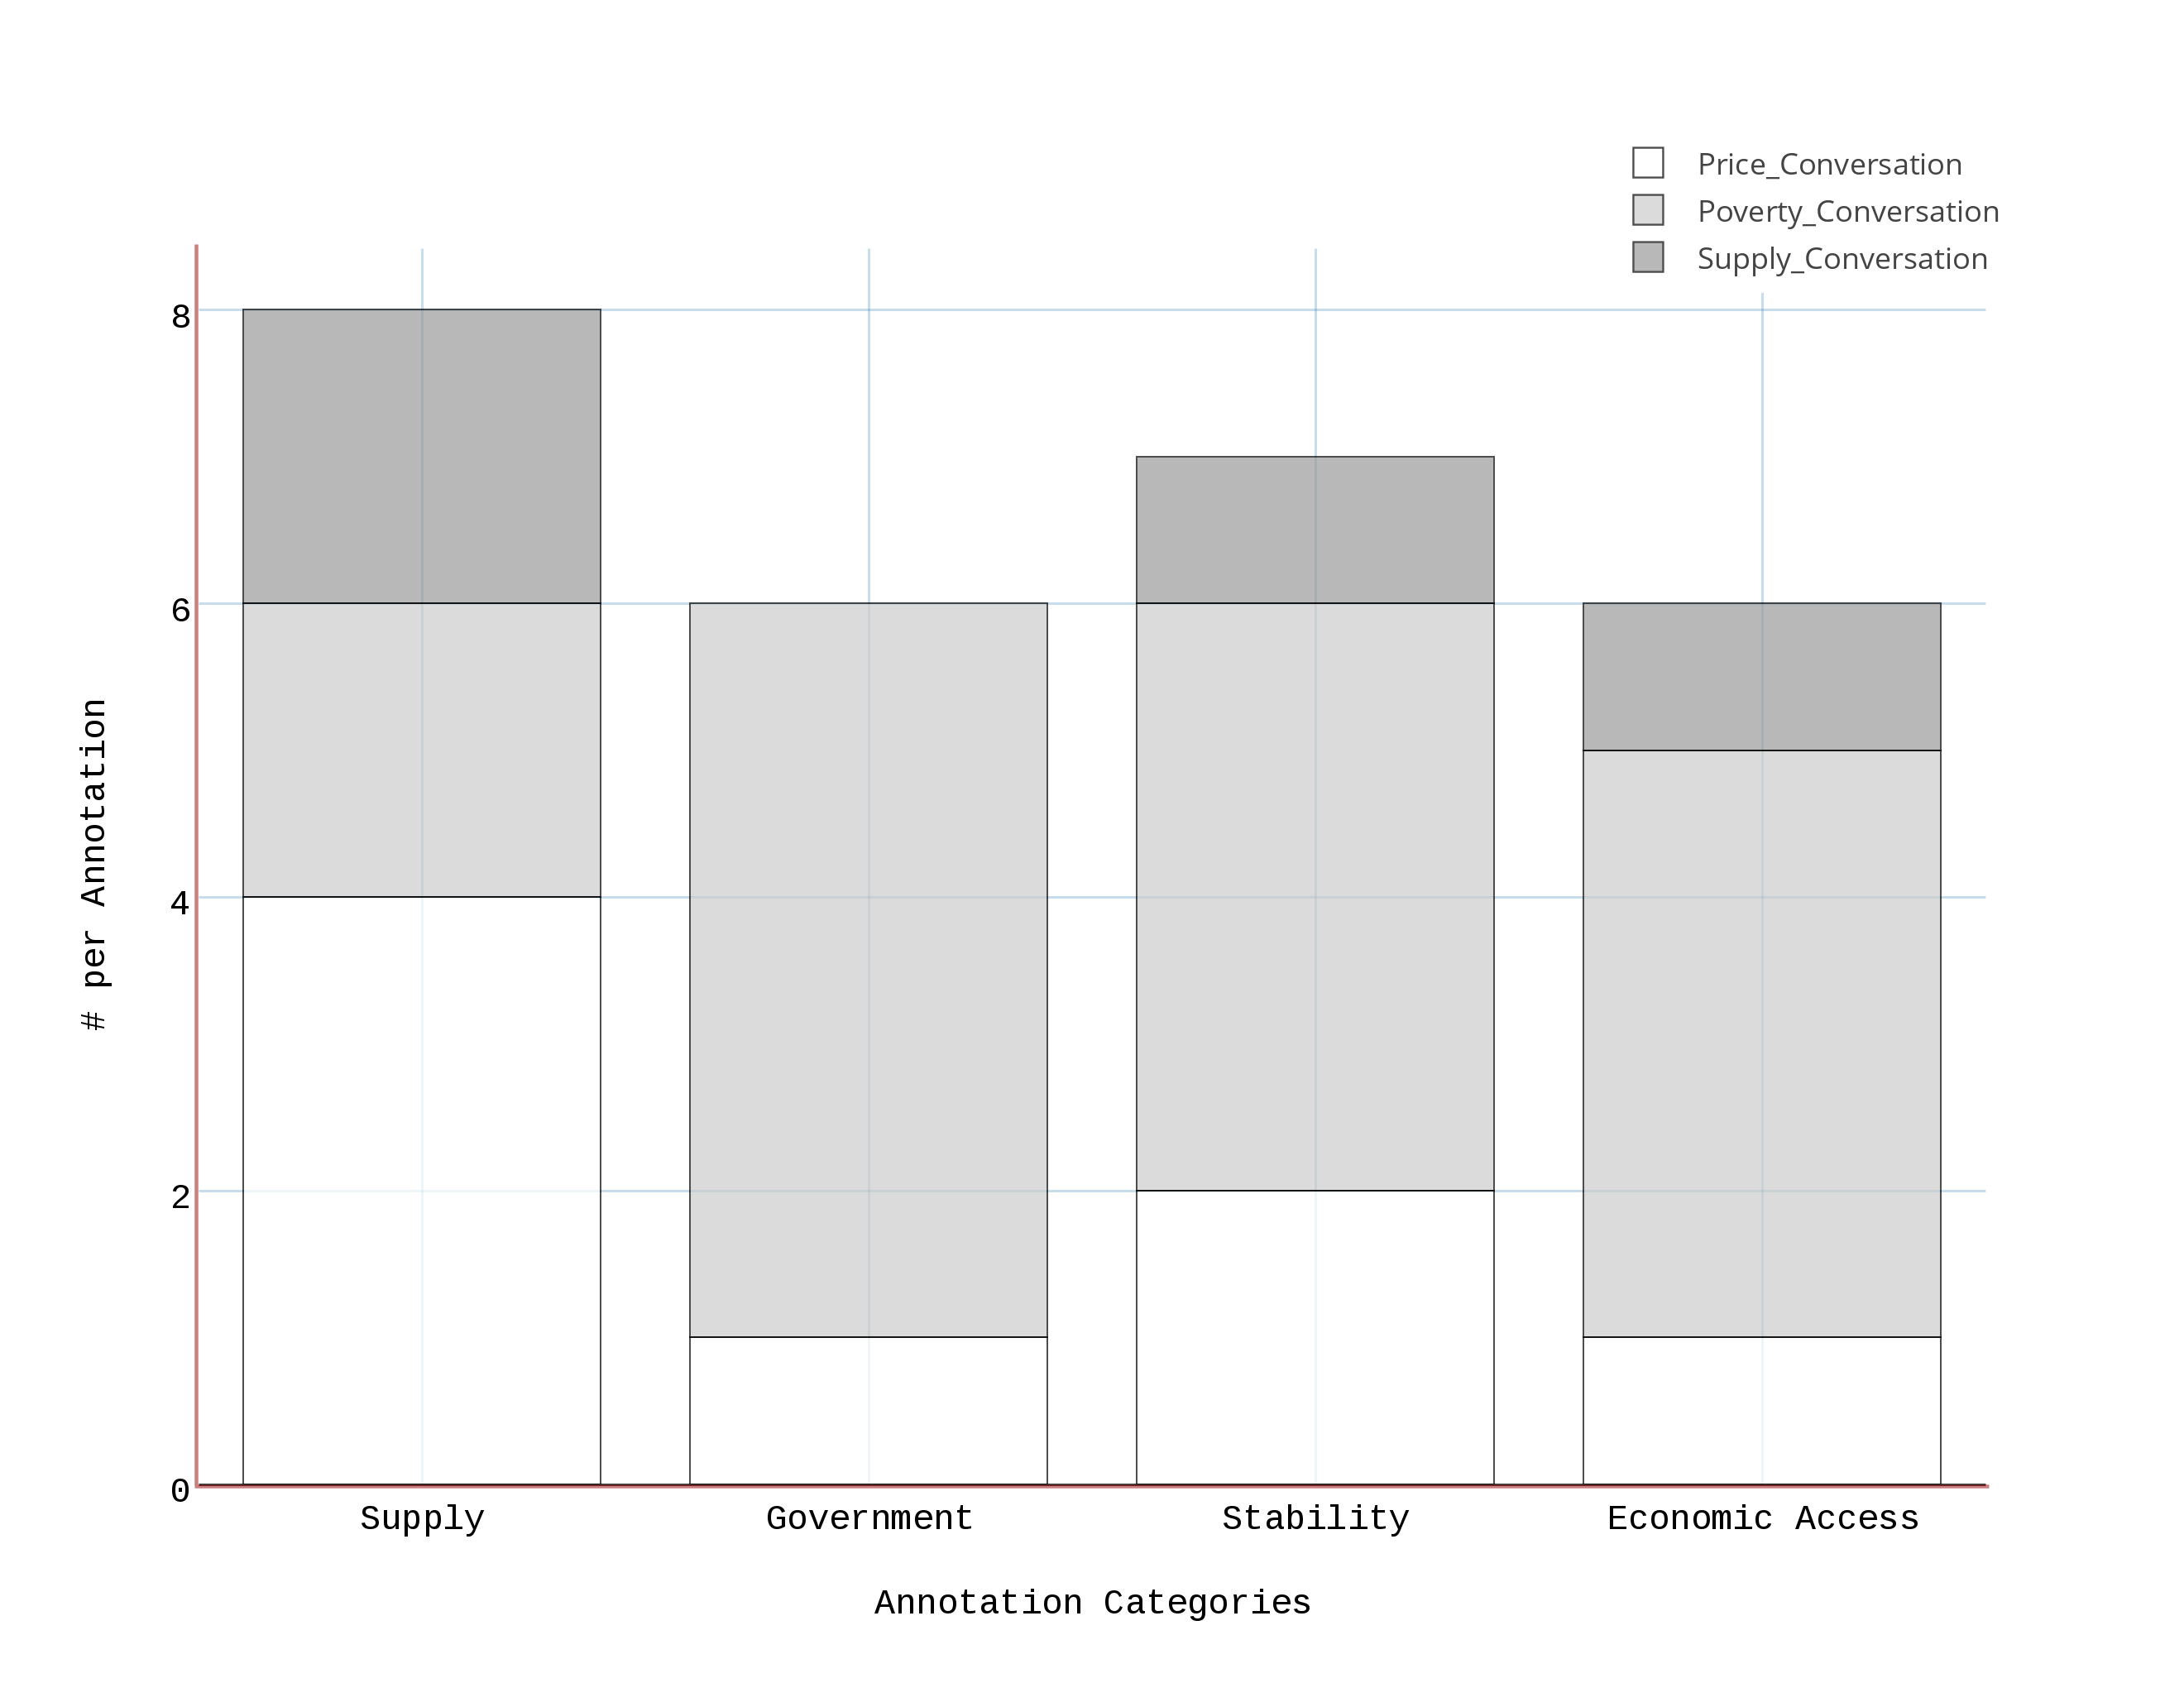
\includegraphics[width=0.7\textwidth ]{img/anal/annotation_dist}
              
        \caption{Annotation Distribution - Relevant to Food Security}
        \label{fig:annotation_dist}
\end{figure}


\subsection{Discussion}

Extracting information from noisy and unstructured text has shown to be a very difficult task. Despite our various filtering attempts there is still a substantial amount of noise in our food security discussions. As most of the volatility was attributed to unrelated topics we will have to rethink the way we use the Twitter data as a feature in our model. Unrelated does not necessarily mean irrelevant. Even Twitter discussion outside our food security objectives can provide valuable information. Most commonly this is achieved by analysing the attitude of a tweet's author. We will hence explore the entropy of sentiment in explaining volatile food prices. 


\chapter{Forecasting Model}


This chapter applies the insights gained in Chapter \ref{4} and makes a practical case on how we can use Twitter as an early warning system for food security threats by means of time series forecasting. First we  outline the methodology of our time series prediction followed by a discussion on the different input models we used. We further highlight details towards the data preprocessing and how we train our model. Lastly,  we present some basic concepts that will aid the reader in understanding the dynamics of the predictions and ultimately help to comprehend the results.  

\section{System Overview}

In Figure \ref{fig:system_architecture} we present a conceptual overview of our proposed system.  A clear understanding of the problem and knowing which variables are capable of explaining the variance is important for accurate predictions. We create different features from the historical price of the commodities and the filtered social media data. To asses the predictive value of the features we run a feature selection algorithm Relief. The proposed set is used as our input and later served to the prediction model. First however we normalize the data and in a second instance perform a smoothing of the input signal. Not illustrated in this image is an additional optimisation procedure we performed for the social media data. We assume that a causal relationship exist between the twitter data and the price. Given this assumption we investigate at which point in history the social media data correlates the most with the given price data. We discuss the particular case of the social media features in Section \ref{}. It is common practice to divide the data into three distinct sets namely train, validation and test. Due to the sparsity of the available social media data we restrict ourselves to a train and test set. The reader should note that the value of the train set is not static. As we discuss in Section \ref{} the training set is updated every 28 days to include recent values. The fourth and final step constitutes the actual model.  Roughly the prediction model ANFIS performs four steps. Fuzzification corresponds to the process of transforming a value between 0 and 1 into grades of membership of linguistic terms. Since the number of linguistic rules is exponential to the number of input values we perform a clustering of the rules. In the third sept those rules are evaluated and eventually transformed into a scalar value between 0 and 1. The output is the predicted value of the price of a commodity. 



%We discussed the first instance Data Acquisition thoroughly in Chapter \ref{3} but wish to highlight that the data is split into train and test set which is a common procedure for supervised learning algorithms. The box bellow illustrated the different transformation procedures applied. . Following the data transformation we create different features from the historical price of the commodities and the filtered social media data. To asses the predictive value of the features we run a feature selection algorithm Relief. The proposed set is used as our input and served to the prediction model illustrated in the last instance of the figure. 


\begin{figure}[H]
        \centering
         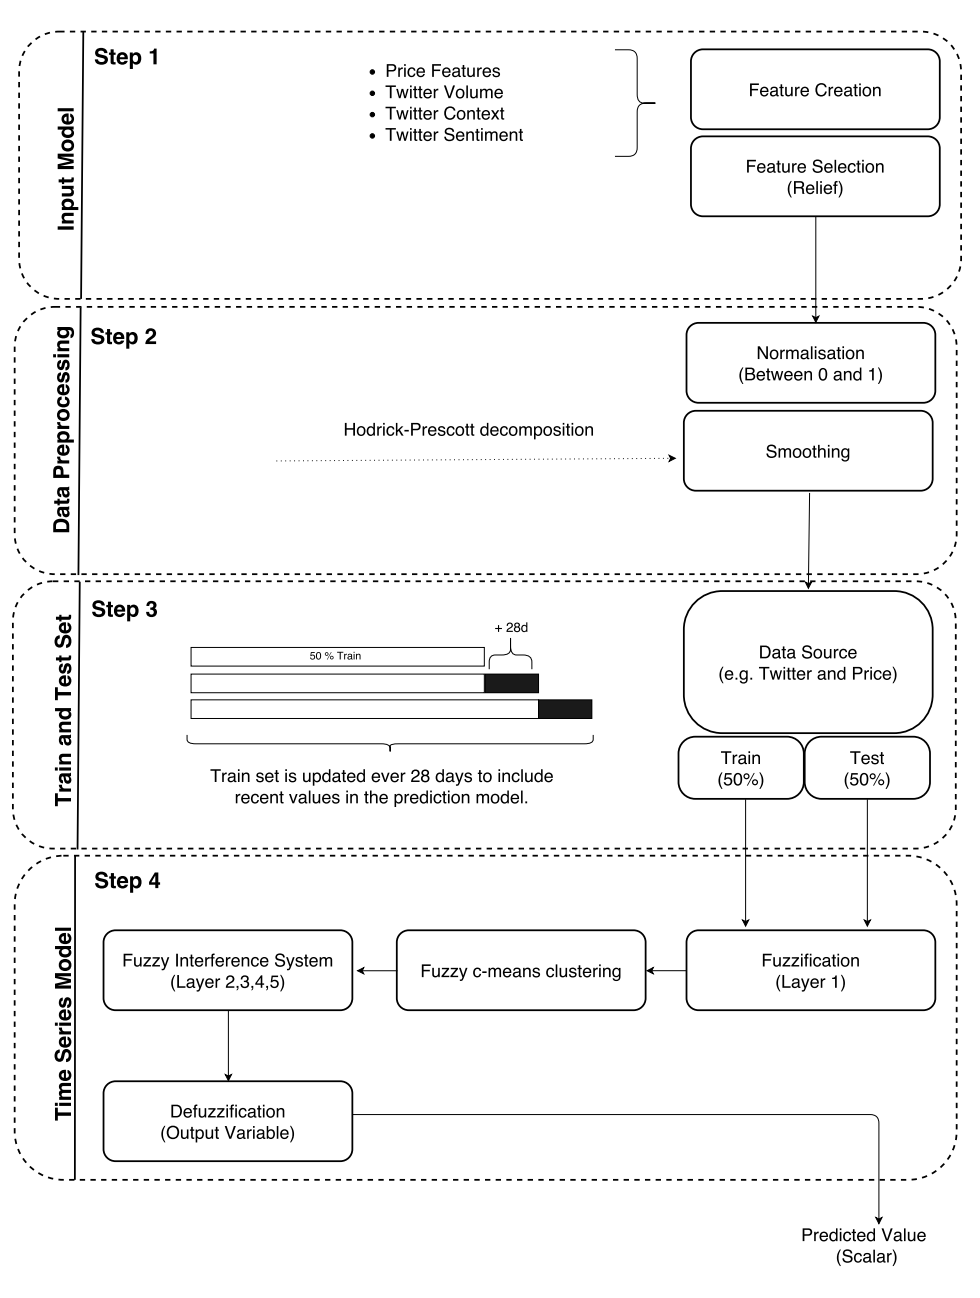
\includegraphics[width=0.6\textwidth ]{img/model/architecture}
              
        \caption{Forecasting - System Overview}
        \label{fig:system_architecture}
\end{figure}



\section{Input Model}

Critical to the success of the model is choosing the right set of features to represent the sample. This is however an extremely challenging task which is one of the reason why we use ANFIS, namely to detect complex nonlinear relationships. Nonetheless   economic theory can help to create representative features. Generally speaking good features should be informative and for our particular task be able to discriminate between rising and falling prices. Given the above named challenges we try to  motivate the choice of features by either referring to past work or relying on economic theory. An input model selection algorithm will aid our attempt of selecting a representative set of features.For benchmarking purposes we create three different models. The first model consists of price features, the second model uses social media features and the last model constitutes a combination of the both. In this section we first describe the features we extract and later define the three input models. 

\subsection{Features}

In the following sections we present two types of price features (spot price and moving average) and three different social media features (attention, context and sentiment ratio).

\subsubsection{Price Feature}

Yao et al. \ref{Yao00acase} suggests that the market can be categorised using the major trends, the intermediate trends and the minor trends. By major trends we refer to trends that last more than a year, and by intermediate trends anything between three weeks to three months. We capture such trends by taking the moving average of one week, two weeks and one month respectively similarly to Yao's model. Given the limited time frame we chose to exclude major trends. We further consider all days preceding the horizon 30 days into the past as potential features. Moving averages are used to remove the day to day instability and extract the underlying trend\cite{armstrong01}. The below Table \ref{tab:inputModel} illustrates the values assigned to each feature. $x$ is the value of today and $x-1$ is a value one day in the past. $\mu(]x-y;x])$ symbolises the moving average of the past $y$ days. 


\begin{table}[H]
\centering
\begin{tabular}{ |c|c|c| } 

 input \# & name & value \\ 
  \hline
 1 & D1 & x \\ 
 2 & D2 & x -1 \\ 
 :& : & : \\ 
  :& : & : \\ 
  :& : & : \\ 
  30 & D30 & x - 29\\ 
  31 & W1 & $\mu(]x-7;x])$ \\ 
  32 & W2 & $\mu(]x-14;x])$ \\ 
  33 & M1 & $\mu(]x-30;x])$ \\ 
 

\end{tabular}
\caption{Input Model: Benchmark Prediction}
\label{tab:inputModel}
\end{table}


\subsubsection{Social Media Features}
\label{SM1}



In Section \ref{corr_results} we rejected the hypothesis that a linear relationship exists between the volume of food tweets and the price of a commodity. However, John Bollen et al. \cite{john11} showed that Twitter conversations have a nonlinear relationship with the movements of the financial markets. Hoping to find a similar relationship for commodities  we consider social attention on different granularities by measuring the volume of the category, subcategory and the product \ref{food_lex}. We further include products that are not specific to a commodity but show a strong linear relationship with the commodity price (i.e. we consider goat as a feature for beef despite it not being a beef product). For beet we consider the twitter volume of the products salami and goat, for wheat we consider the twitter volume of gluten and noodles and lastly for milk we consider the twitter volume of the products mozzarella and cheshire. All of those products were found to have a significant correlation with the commodity price. 
 
 In general microblogs capture one topic due to its 140 keyword limitation. The topics can usually be inferred by capturing one or two keywords. However certain terms are more intrinsic than others i.e. the keyword \emph{IBM} can unambiguously be related to the company whereas the  term \emph{break} has multiple meanings and given the context, could be unrelated to a desired topic. We hence introduce the notion of contextual sensitive Tweets. Tweets considered contextual sensitive match both a term in the Food Lexicon and the Predictor Lexicon. We consider the context of food price, supply, poverty and needs \ref{pred_lex}. 
 
 Despite having identified a significant correlation for contextually sensitive Tweets our analysis in Section \ref{conversation} concluded that unrelated topics mostly drive the attention volatility. Public mood states or sentiment might hence be a more valuable indicator. This intuition is supported by \cite{nofsinger05} namely that emotions and mood do not uncommonly drive financial decisions. For the purpose of this analysis, we consider different ratios of sentiment. The ratio between the numbers of positive and negative Tweets \cite{Nguyen12}, the proportion of neutral and total Tweets,  the ratio between the numbers of non-neutral and total posts \cite{Zhang09}, the ratio between the number of positive and negative discussions and lastly the ratio between the numbers of neutral and non-neutral messages. 

Table \ref{tab:socio_feat} concludes our input model. We measure the sentiment for both Twitter buzz and contextually sensitive Tweets. To uniquely identify from which category we are measuring the sentiment  \# refers to a unique identifier. The result is an input model with 51 features. \footnote{ (1 $\times$ attention for each food category (3) + 1 $\times$ attention for products with high correlation (2) + 1 $\times$ attention for each context (4) +  6 $\times$ sentiment ratio of each food category (18) + 6 $\times$ sentiment ratio of each context (24) =  3 + 2 + 4 + 18 + 24  = 51 ) }
 

\begin{table}[H]
\centering
\begin{tabular}{ |p{5cm}|p{2cm}|p{7cm}| }



 Feature Type & Name & Value    \\
\hline
Attention & AC\# & \#Commodity   \\
\hline
Context & CP\# & \#Price f. Commodity   \\
        & CS\# & \#Supply f. Commodity  \\
        &CP\# & \#Poverty f. Commodity   \\
        &CN\# &\#Need f. Commodity  \\



  \hline
   First Sentiment Ratio & SR\#& \#positive : \#negative Tweets  \\
  Second Sentiment Ratio & SR\# & \#positive : \#(positive + negative) Tweets   \\
  Third Sentiment Ratio& SR\#  & \#negative: \#(positive + negative) Tweets  \\
   Fourth Sentiment Ratio  &SR\#   & \#neutral : \#(positive + negative) Tweets  \\
   Fifth Sentiment Ratio &SR\#  & \#(positive+negative) : \#all Tweets   \\                 
    Sixth Sentiment Ratio  &SR\#  & \#neutral : \#all Tweets \\
                          

   


\end{tabular}
\caption{Input Model: Social Media Prediction}
\label{tab:socio_feat}
\end{table}



\subsection{Feature Selection}

We aim to find the most significant features among the 33 price and the 51 social media features to decrease the complexity and lastly improve the prediction accuracy. We perform the model selection for all three models (e.g. price, social media and mixture model). For that purpose, we used a feature selection algorithm Relief \cite{kira92} \cite{kono94} \cite{Robnik97} that allows us to distinguish relevant from irrelevant features were relevance is measured on how much influence a feature has on the output value. Relief finds relevant features using a heuristic where the evaluation is performed on a distance measure. The data instances of the features belong to different classes. We measure the relevance of a feature $f_x$ by measuring the distance from the nearest neighbour of each class to $f_x$. The nearest neighbour of the same class (same class as $f_x$) is called nearest hit, and the nearest miss is the closest neighbour of a different class.  The heuristic is computed for each feature in Equation \ref{eq:heuristic_new}.

\begin{equation} \label{eq:heuristic_new}
W_i = W_i  - (x_i - nearestHit_i)^2 + (x_i - nearestMiss_i)^2
\end{equation}

A feature is considered irrelevant or redundant if $W_i \leq 0$, that is if the difference between the same class is higher than the one of a different class.  We measure the most significant features with respect to the horizon of four days, seven days and 14 days. Furthermore, we consider three different commodities, wheat (w), beef (b) and milk (m).


\subsubsection{Price Model}

The model selection is performed on the input values illustrated in Table \ref{tab:inputModel}. The configuration \emph{w-4} in the Table \ref{tab:feat_mod1} refers to wheat with a prediction horizon of four days. The most predictive features are  1.) $\phi_1$ : $D30$ , 2.) $\phi_2$ : $D29$,  3.) $\phi_3$ : $D28$, 4.) $\phi_4$ : $W1$ , 5.) $\phi_5$ : $D27$ and 6.) $\phi_6$ : $D26$.

The numbers in the Table \ref{tab:feat_mod1} refer to the relative importance of the feature for a specific configuration. The higher the value, the more predictive the feature is considered to be. It is interesting to observe that Relief consistently suggested the same features irrespectively of the commodity type and the prediction horizon. This gives us a strong confidence in the relative importance of the prediction task at hand, as it generalises well over different models i.e. horizons and also different commodities. We can see that the values follow a clear trend. With an increasing horizon, the features lose its importance as the prediction task becomes more and more challenging. 

For our prediction task, we consider the top 10 features \footnote{We performed experiments with five,10 and 20 features and found that 10 features yield the highest prediction accuracy. A better predictions can be expected with more than 10 features however at some point the model will overfit. We leave an extensive search of the optimal number of features for future work.}.Those additional features ($\phi_7 - \phi_10$) not displayed in Table \ref{tab:feat_mod1}  are for most commodities and horizons the same but ranked in different orders depending on the prediction task. Interestingly D25, D24, D23 and W2 rank highly along the other values in Table \ref{tab:feat_mod1} which are all placed in the intermediate past. This observation suggests that models based on the intermediate past poses more predictive power and outperform strategies based on features in the recent past. Robert Marx also observed this effect and investigated the hypothesis in \cite{iuj11}. His conclusion was that models with intermediate variables tend to outperform such only considering recent values. A possible explanation mentioned in the paper is that such variable best captures the momentum of a commodity price. 




\begin{table}[H]
\centering
\begin{tabular}{ |p{2cm}|p{1cm}|p{1cm}|p{1cm}|p{1cm}|p{1cm}|p{1cm}|p{1cm}|p{1cm}|p{1cm}| }
  \hline
 Feature & w-4 & b-4 & m-4 & w-7 & b-7 & m-7 & w-14 & b-14 & m-14   \\
 \hline

 $\phi_1$ & 0.0624   & 0.0212   & 0.0310 &  0.0586  & 0.0197 & 0.0300 & 0.0487 & 0.0155 & 0.0271\\
  \hline
  $\phi_2$ & 0.0558 & 0.0193 & 0.0281 & 0.0513 & 0.0175 & 0.0268 & 0.0411 & 0.0132 & 0.0237 \\
  \hline
  $\phi_3$ & 0.0495 & 0.0174 & 0.0253 & 0.0444 & 0.0153 & 0.0236 & 0.0343 & 0.0111 & 0.0205 \\
  \hline 
  $\phi_4$ & 0.0440 & 0.0157 & 0.0227 & 0.0388 & 0.0135 & 0.0209 & 0.0291 & 0.0093 & 0.0179 \\
  \hline 
  $\phi_5$ & 0.0434 & 0.0156 & 0.0225 & 0.0381 & 0.0133 & 0.0206 & 0.0283 & 0.0091 & 0.0175 \\
  \hline
  $\phi_6$ & 0.0378 & 0.0138 & 0.0198 & 0.0324 & 0.0114 & 0.0178 & 0.0231 & 0.0074 & 0.0149 \\
  \hline
 \end{tabular}
\caption{Feature Selection: Benchmark Prediction}
\label{tab:feat_mod1}
\end{table}


\subsubsection{Social Media Model}

In this section we select among the features displayed in Table \ref{tab:socio_feat} to build the input set of our social media model. Again we try to find features that generalise well among different commodities and horizons. The acronyms (e.g. AC50) used in this section correspond to the ones introduced in Section \ref{SM1}. The number is used as an index to distinguish sentiment ratios of different food categories. 

In the previous section we showed that input variables for the price model generalise well among all commodities and price horizons. On the other hand social media features seem to be more specific to a given task and commodity. For the top 16 features, we only found three features that were present in all commodities and all horizons or in other words were able to generalised well. Among the three were the attention count of the selected products that showed a high correlation in our analysis (AC50),  the first sentiment ratio of poverty (SR32) and the first sentiment of the subcategory (SR15). Other features that generalised well for all prediction tasks of a given commodity were the second sentiment of the subcategory (SR16),  the second sentiment of poverty (SR33), the fourth sentiment of poverty (SR35), the first sentiment of price (SR38), the second sentiment of supply (SR45), the sixth sentiment of supply(SR49) and lastly the attention count of another selected product that scored well in our correlation analysis (AC51). The top features along with the Relief score for each given commodity are illustrate in Table \ref{tab:feat_mod2}. 
The sentiment of the tweets together with the attention counts of products that showed a high correlation in Section \ref{corr_results} seem to be expressive for the price variation. Especially the sentiment features for discussions centered around poverty rank highly. Our qualitative analysis in \ref{an_result} showed that twitter conversation for poverty discussion had the highest relevance. We would like to point out that no features built on discussions centered around food needs were selected. This again correlates with our analysis in previous sections where we concluded that non of the volatility in the needs discussion was caused by topics relevant to food security.  Admittedly, it is not a decisive indicator of the quality of the feature. However, it might explain why poverty features rank so highly. 


\begin{table}[H]
\centering
\begin{tabular}{ |p{2cm}|p{1.5cm}|p{1.5cm}|p{1.5cm}|p{1.5cm}|p{1.5cm}|p{1.5cm}|p{1.5cm}|p{1.5cm}|p{15cm}| }
  \hline
 Feature &  $\phi_1$ &  $\phi_2$ &  $\phi_3$ &  $\phi_4$ &  $\phi_5$&  $\phi_6$    \\
 \hline

 $wheat$ & AC50 (0.2119)   & SR32 (0.2294)   & AC51 (0.2121) &  SR35 (0.1356)  & SR16 (0.1385) & SR15 (0.1385)\\
  \hline
  $beef$ & AC50 (0.2210) & SR45 (0.1389) & SR32 (0.1323) & SR33 (0.1339) & SR38 (0.1339) & SR44 (0.12826)  \\
  \hline
  $milk$ & AC50 (0.3339) & AC51 (0.1774) & SR45 (0.1774) & SR38 (0.1413) & SR35 (0.1313) & SR49 (0.1013)  \\

  \hline
 \end{tabular}
\caption{Feature Selection: Benchmark Prediction}
\label{tab:feat_mod2}
\end{table}



\subsubsection{Mixture Model}

Combining the price and social media features from Table \ref{tab:inputModel} and Table \ref{tab:socio_feat} we want to investigate if Relief proposes as similar set as for the separate models or if the combined model favours a different group of input variables. Only a few features generalised well over all commodities which is why we focus our search of finding input variables that are specific to beef, milk and wheat but generalise well over different prediction horizons. As in our price model, days in the intermediate past were proposed for all three commodities. The ratio varies strongly among the commodities. Beef favours price variables where milk and wheat have a majority of social media features. We observe an interesting trend, namely that all commodities favour supply and needs feature over price and poverty which is very different to the pure social media model. We assume that the price data made the conversations about price more obsolete. To conclude the proposed features are the fourth and the fifth sentiment ratio of the product (SR11, SR12), the fourth, fifth, sixth sentiment ratio of needs (SR29, SR30, SR31), the third sentiment ratio of poverty (SR34), the first, third sentiment ratio of price (SR38, SR40) and lastly the second, third sentiment ratio of supply (SR45, SR46). The price features are all days of the last week i.e. (D24, D25, D26, D27, D28, D29, D30) and the moving average of the past week (W1). 

\begin{table}[H]
\centering
\begin{tabular}{ |p{2cm}|p{1cm}|p{1cm}|p{1cm}|p{1cm}|p{1cm}|p{1cm}|p{1cm}|p{1cm}|p{1cm}| p{1cm}|  }
\hline
$milk$ & SR38 & SR40 & SR45 & D30 & D29 &  SR34 & SR12 & SR47 & SR46 & SR11 \\
\hline
$beef$ & SR38 & D30 & D29 & D28 & D27 &  W1 & D26 & SR45 & D25 & D24 \\
\hline
$wheat$ & D30 & D29 & SR22 & SR29 & SR30 & SR31 & SR15 & SR16 & SR33 & SR14 \\
\hline
\end{tabular}
\caption{Feature Selection: Benchmark Prediction}
\label{tab:feat_mod3}
\end{table}





\section{Data Preprocessing}
\label{dataprocessing}

Before feeding the data into our prediction model, we analysed and cleaned the data. The representation of the data is of great importance to assist ANFIS in learning the relevant patterns. In a first instance, we had to match both the time series of the Twitter data with the time series of the price data. During weekends and national holidays the markets are closed, hence we  removed such instances from the Twitter data. The commodities beef, milk and wheat are traded on different commodity markets. We observed that some of the markets had different closing days i.e. some markets considered a day a holiday, some others not. For wheat and cattle we removed the 12/11/12 and the 8/10/12 which are the Veteran day and the Columbus day respectively to match the price data of milk. Secondly, we proceeded to interpolate zero values. Some of the price data sets showed values of zero on days that were neither weekends nor holidays. Similarly, the Twitter archive did not contain Twitter data for some time periods. We linearly interpolated such missing values by solving and approximation to the partial differential equations \cite{john2012}. Fuzzy Interference Systems expect an input of a unit interval i.e. between 0 and 1. We hence normalised the data as illustrated in Equation \ref{normalize}. Min and Max are the lower and upper bounds of data set where $\alpha$ is a small constant we introduced to avoid zero divisions. The Fuzzy system expects a unit interval to avoid losing its sensitivity towards smaller scaled features. 

\begin{equation} \label{eq:normalize}
\overline{ y } = \frac{x - min}{max - min}  + \alpha \end{equation}


Lastly, we performed a smoothing of the data which is in agreement with our objective, namely to be more sensitive to long-term than to short-term fluctuations \cite{edward81}. As we can see in Figure \ref{fig:distribution_smoothing} there are some extreme price increases and drops. By applying the Hodrick-Prescott decomposition \cite{edward81} filter, we receive a distribution that is more normal by avoiding such outliers. Additionally the Figure \ref{fig:distribution_com} illustrates nicely the characteristics of commodities, namely that it is mostly driven by small price changes. 


\begin{figure}[ht]
        \centering
        \begin{subfigure}[b]{0.5\textwidth}
                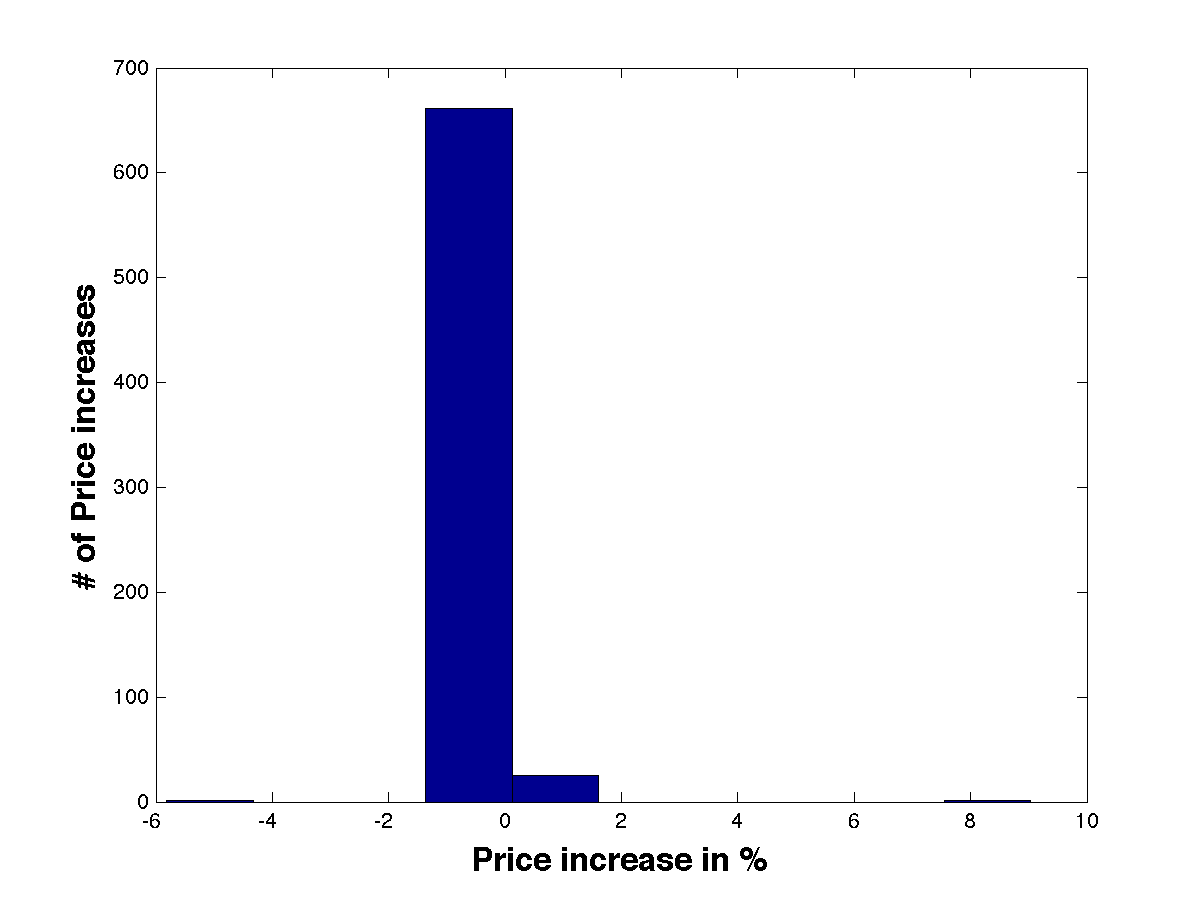
\includegraphics[width=\textwidth]{img/model/p_increase_n_log}
                \caption{Price Increase Distribution without Scailing}
                \label{fig:}
        \end{subfigure}%
        ~ %add desired spacing between images, e. g. ~, \quad, \qquad, \hfill etc.
          %(or a blank line to force the subfigure onto a new line)
        \begin{subfigure}[b]{0.5\textwidth}
                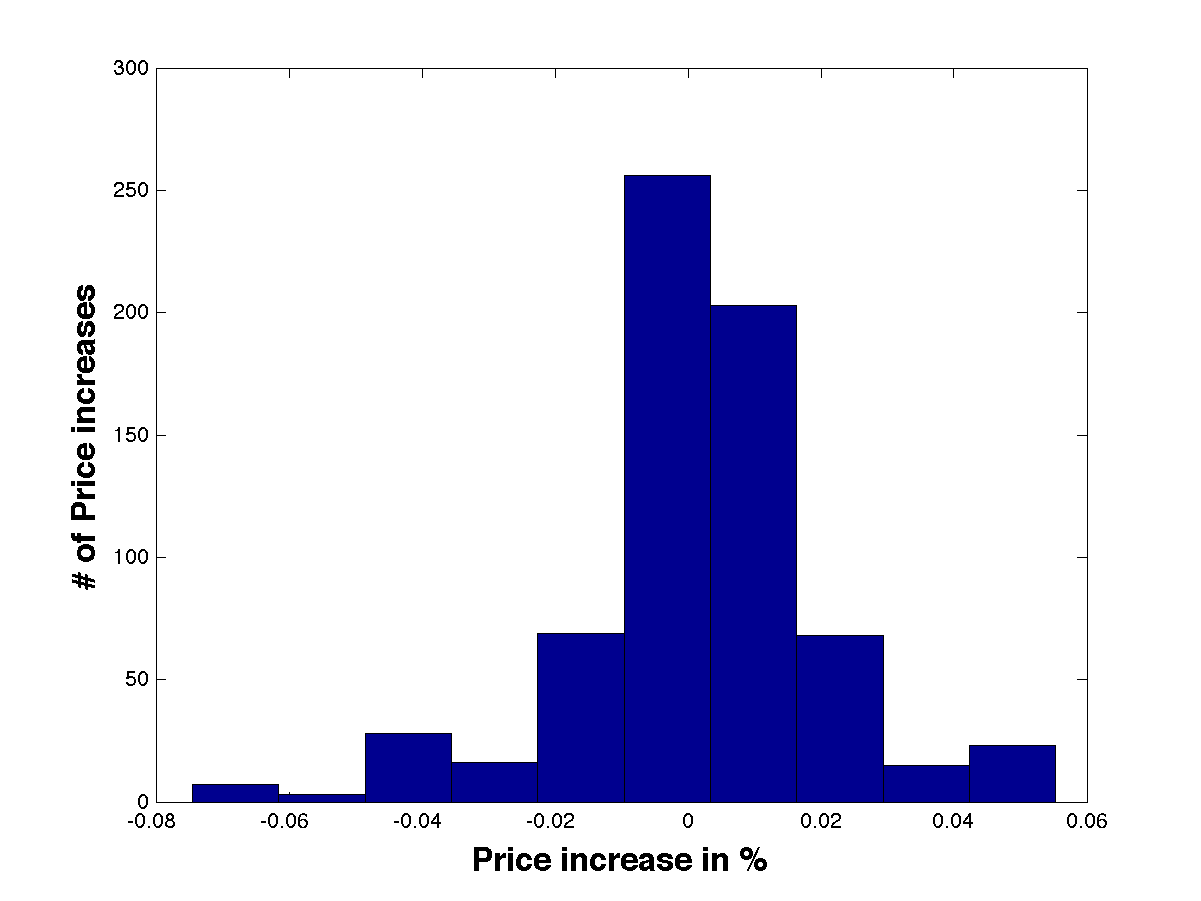
\includegraphics[width=\textwidth]{img/model/p_increase_w}
                \caption{Price Increase Distribution with Scailing}
                \label{fig:u_log}
        \end{subfigure}
        ~ %add desired spacing between images, e. g. ~, \quad, \qquad, \hfill etc.
          %(or a blank line to force the subfigure onto a new line)

      
        \caption{Characteristics of Commodity Price Data}\label{fig:distribution_smoothing}
\end{figure}





\section{Training the Model}

For training and testing our model, we choose the period 03.01.2012 - 26.09.2014. We thought of numerous ways to test and train our model. Different approaches have been suggested by Ibeling Kaastra \cite{Kaastra96designinga}. Most commonly the data is split into a train set, validation set and lastly a test set. The model is trained once in a batch fashion and used for all future predictions. Such an approach can be dangerous particularly when one considers historical data reaching far into the past. Market conditions might have been different then and might not apply to future predictions. Choosing a particular time frame can be a bad idea as well. Consider the training data only exhibiting an upwards trend the model will then not generalise well for declining prices. Yao et al. \cite{Yao00acase} proposed to use statistical methods to investigate the best period for training the network. However to make any statistically significant claims we need more than 2.5 years of historical data. Lastly, Ibeling Kaastra describes a method called the walk-forward or sliding window approach. This approach involves creating overlapping sets of a train and test data. Each set is moved forward through the time series to test the robustness of the model. This framework addresses the concern raised regarding including data from far in the past that might not reflect the current market conditions and is widely used for commodity predictions \cite{Kaastra96designinga}. We decided to apply a variant of the sliding window approach and train or model in an online fashion. Given the limited amount of data we choose not to exclude any data from future prediction. However, to be able to adapt to new market conditions we increase the training and validation window as we move along the timeline. We used the first 50 \% of the data to train the model. 


\section{Time Series Model}
\label{fuzzy_model}

In this section, we present the terminologies and concepts around Fuzzy logic, focusing on the basics of Fuzzy variables and Fuzzy sets. We further derive a Neural network with a Fuzzy interference system (FIS). 

\subsection{Motivating a Fuzzy Approach for Time Series Modelling}

Compared to other approaches, Fuzzy logic has seen only a few applications in forecasting despite its promising results. We hence want to motivate the use of this technique in further detail. Fuzzy logic was initially proposed to provide a framework for imprecise reasoning. Zadeh \cite{Zadeh65} introduced the concept to describe real world phenomena that do not have a precise description of a membership class. Another branch of mathematics that deals with uncertainty is the field of probability. However, there is a distinct difference between the two. Probability theory is based on Bivalent logic, which means every proposition is either true or false. Only certainty is a matter of degree, which brings us to an important distinction. In Fuzzy logic, everything is a matter of degree, which is ultimately how we perceive the real world. \say{This form of reasoning allowed the development and analysis of systems by expressing the qualitative aspects of human reasoning without using any complex mathematical models} \cite{Jang91}.  In some areas such as time series prediction techniques such as ARMA and AR, have shown clear limitations \cite{box90}. Nonlinear approaches, such as Adaptive Neuro Fuzzy Inference System (ANFIS), have proven to be more successful \cite{chap04}. Prediction accuracy is however not the only concern in forecasting models. Understanding the behaviour and gaining insight into the underlying dynamics is equally important \cite{neil93}. This makes ANIFS especially appealing. Not only does it poses strong predictive capability but as a consequence of its rule-based design it allows for interpretability of the predictions. The interpretability is particularly important as the results might help us better understand the determinants of food security risks in social media. 



\subsection {Fuzzy Variables and Fuzzy Sets }
\label{fuzzification}

Zadeh \cite{Zadeh65}  defined Fuzzy variables as attributes that distinguish between elements of some universe of discourse. He uses the colour of an object as an example. Each colour has a wavelength, which is a precise numerical definition. In natural language, we tend to classify colours not by its numerical value, but by colour objects (e.g. red, blue, green). Colour objects fall within the scope of a specific wavelength or how it is commonly referred to in Fuzzy logic,  a Fuzzy set. Red or blue describe the object's colour, but it is by no means a precise definition. By applying a membership function, we can precisely define the colour in a range between zero and one. This whole prrocess is commonly referred to as Fuzzification and is the initial step of the system as illustrated in Figure \ref{fig:system_architecture}. The most common membership functions are Gauss function, Trapezium function and the Triangle function. We choose to use a Gaussian membership function defined by Equation \ref{eq:gaus},  as they are differentiable and desirable for optimisation purposes \cite{wu12}. We will refer to $a_i, b_i, c_i$ as the parameter set.  

\begin{equation} \label{eq:gaus}
\mu_A(x) =  \frac{1}{ 1 + |\frac{x- c_i }{a_i}|^{2b_i}  }\end{equation}


Concerning our Fuzzy logic system, we will distinguish between an input variable and output variable. The output variable depends on the input value's corresponding membership function and a decision matrix, where we will explain the later in the following Section \ref{fis}. 

 To illustrate the two concepts Fuzzy logic and Fuzzy sets let us consider Figure \ref{fig:fuzz_example}. The three triangular functions precisely define the scope of each colour object (red, green, blue). The colour object green is exactly green at the point $x_2$ and partly green between $x_1$ and $x_2$ and likewise $x_2$ and $x_3$. 
 
For this exercise, we fuzzily the colour object of a tangerine that is orange.  We define orange to be a little red (where little is a value between 0 and 1) corresponding to $y_r$ and very green corresponding to $y_g$.  The membership function would take orange as input corresponding to $x_i$ and output $y_g$ and $y_r$ which formulate a degrees of memberships to the fuzzy set green and red respectively. This toy example generalises to any other object. The object price can be modelled with the triangular functions high, medium low. Sentiment, on the other hand, would use positive, negative or neutral instead. 




\begin{figure}[H]
        \centering
         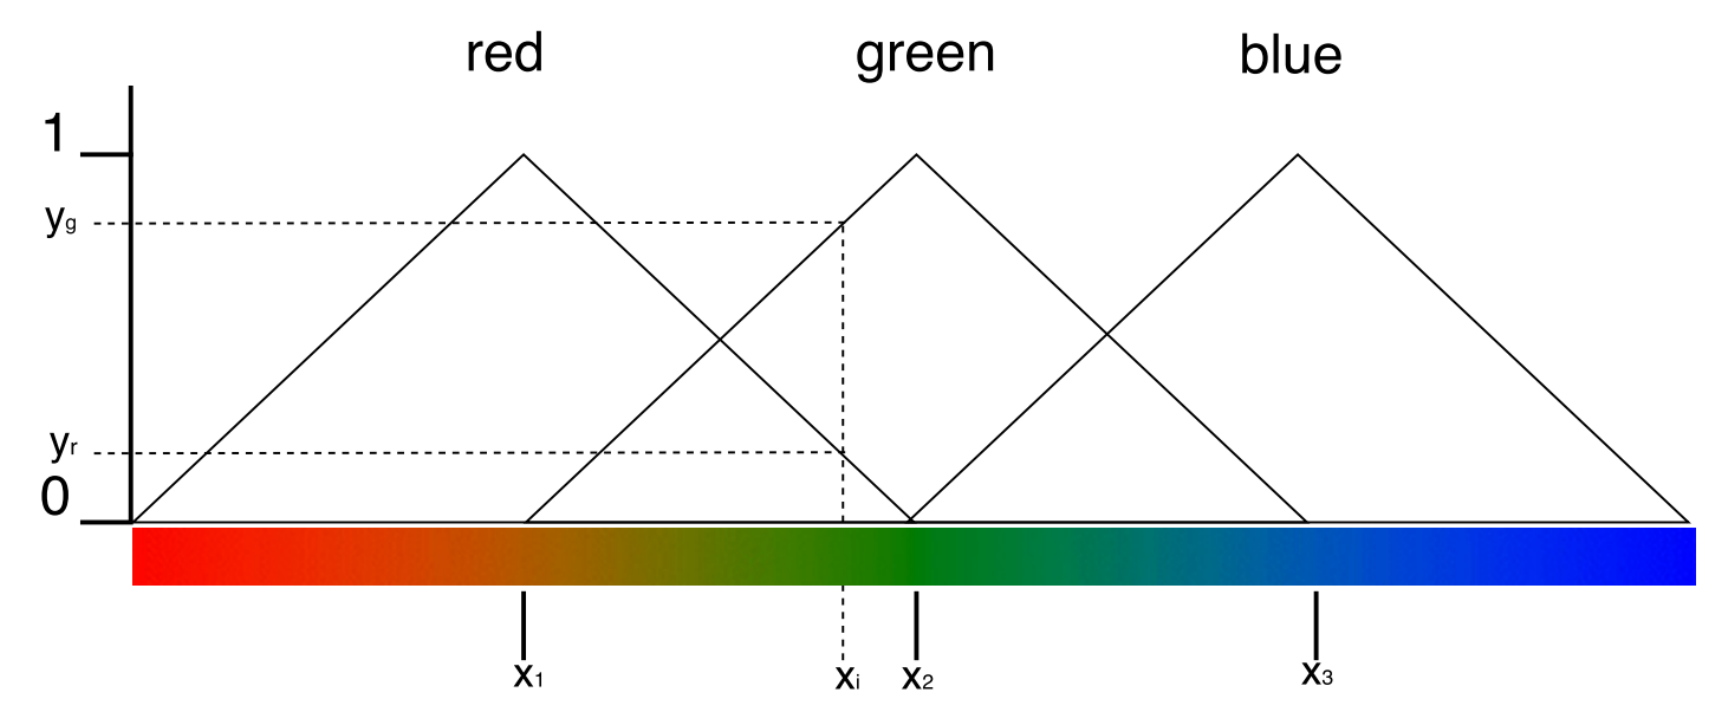
\includegraphics[width=0.7\textwidth ]{img/model/fuzz_example}
              
        \caption{Fuzzy Variables and Fuzzy Sets - A Colour Object Example}
        \label{fig:fuzz_example}
\end{figure}



\subsection{Fuzzy Interference System}
\label{fis}

We first describe the components of the Fuzzy interference system (FIS) and then give intuition on how the system is modelled as a Generalised Neural Network (GNN). 

FIS evaluates a decision matrix composed of rules in the following semantic: \\

\centerline {$ \textbf{IF} <  A  > \textbf{AND} <  B  > \textbf{THEN} < Conclusion > $}

The rule base grows exponentially with the number of variables. Hence, we have to consider carefully the input variables to minimise the complexity and to make the inference reliable. A multivariable system uses two different kinds of connectives to combine the fuzzified values. The union is defined in Equation \ref{eq:union} as the \emph{multiplication} of the membership function of set A $\mu_A(x)$ and B $\mu_B(y).$ The result is a weight $w_i$. $x$ and $y$ are the input variables and could be anything from the attention count of tweets to a sentiment ratio. 


 \begin{equation} \label{eq:union}
 w_i =  \mu_{A\cup B(x,y)} =   \mu_A (x) \times \mu_B(y)
 \end{equation}

The intersection is defined in Equation \ref{eq:probor} as the \emph{probabilistic OR} of the membership function of set A $\mu_A(x)$ and B $\mu_B(x).$ 
\begin{equation} \label{eq:probor}
 w_i =  \mu_{A\cap B(x,y)} =   \mu_A (x)  + \mu_B(y) -  \mu_A (x)  \times \mu_B(y)
 \end{equation}

The output of one Fuzzy Rule is computed by Equation \ref{eq:output}.


\begin{equation} \label{eq:output}
 z = dx + ey + f  \end{equation}
 
In case the output is preferred to be constant rather than linear we set $d$ and $e$ to zero and the constant  $f$ to the desired output of our system. The final output is the weighted average of all rules computed by Equation \ref{eq:finaloutput} where $N$ is the number of rules.

\begin{equation} \label{eq:finaloutput}
Output = \frac { \sum\limits_{i=1}^N  w_i z_i} {\sum\limits_{i=1}^N  w_i } \end{equation}



\subsection{Adaptive Neuro Fuzzy Inference System }

We now model the above-described process as a Neural network illustrated in Figure 5.4.  In \textbf{Layer 1} every node maps the input variables x1 and x2 via the membership function in Equation \ref{eq:gaus} to a Fuzzy Set.  \textbf{Layer 2} applies Equation \ref{eq:union} or Equation \ref{eq:probor} which multiplies the incoming signals and forward the product to the next layer. \textbf {Layer 3} calculates the ratio of the rule's strength to the sum of all rule's strength. We apply the normalisation Equation \ref{eq:normfuzz} in this Layer. 

\begin{equation} \label{eq:normfuzz}
\overline{w_i} =  \frac{w_i}{w_1 + w_2}, i = 1,2 \end{equation}

 \textbf{Layer 4} applies Equation \ref{eq:layer4}, which is similar to Equation \ref{eq:output} but multiplied by the factor obtained in \textbf{Layer 3} from Equation \ref{eq:normfuzz}. 
 
  \begin{equation} \label{eq:layer4}
 \overline{w_i} f_i =  \overline{w_i }(dx + ey + f) \end{equation}
 
 Finally, \textbf{Layer 5} computes the overall output as the summation of all incoming signals through Equation \ref{eq:finaloutput}. The construction yields a network with 5 layers,  16 nodes and 24 parameters (12 in Layer 1, 12 in Layer 4). 
 
 
 
\begin{figure}[H]
        \centering
         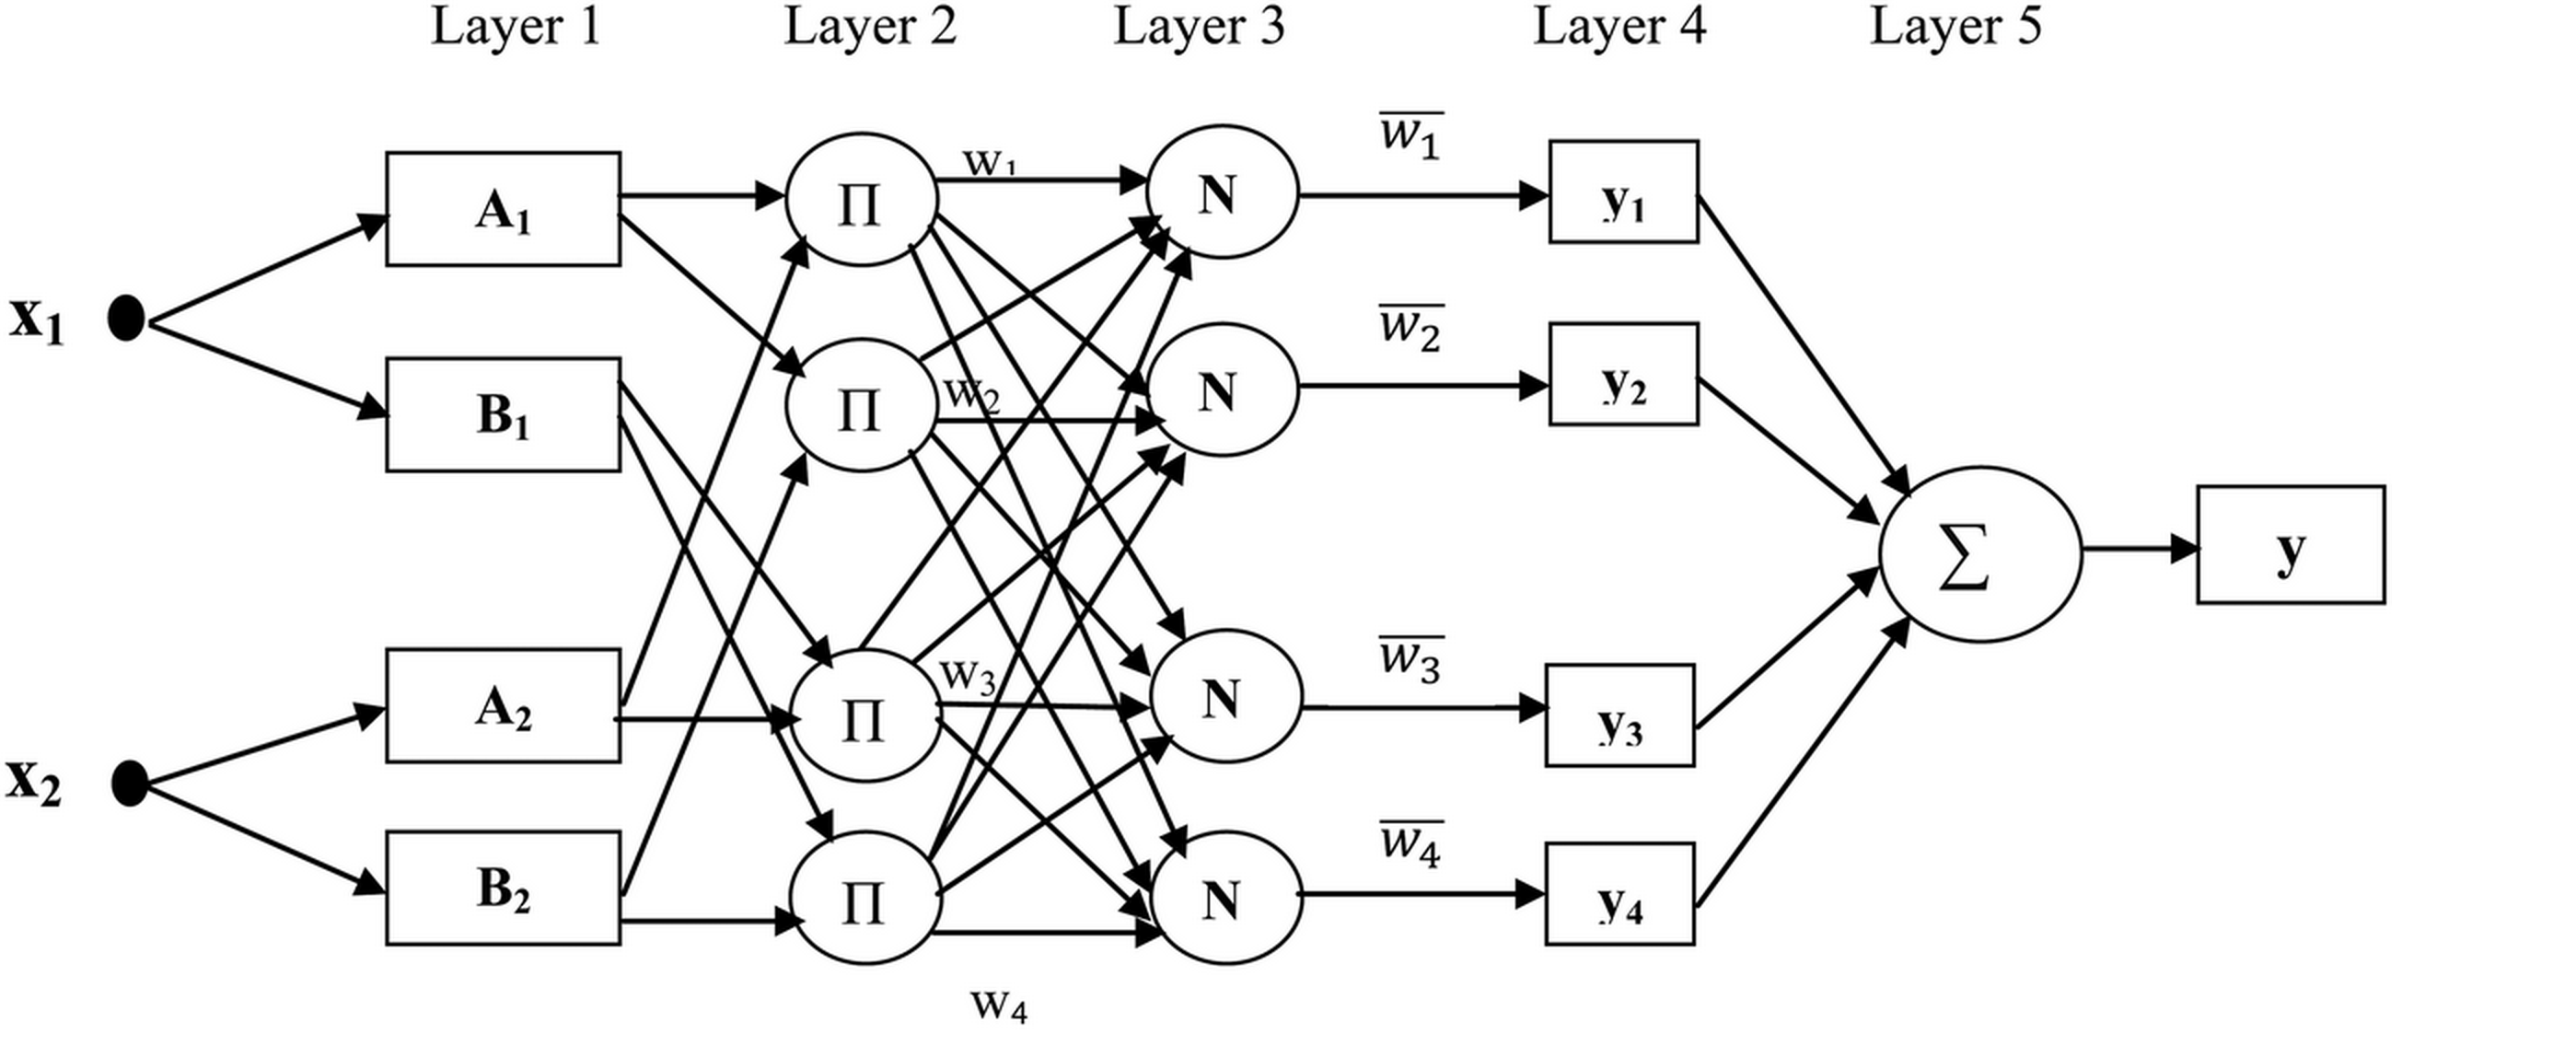
\includegraphics[width=1\textwidth ]{img/model/gnn_fuzz}
         \begin{minipage}{\linewidth}
\caption[Caption for LOF]{Adaptive Neuro Fuzzy Interference System\footnotemark}\label{fig:gnn_fuzz}

\end{minipage}      
       
        
\end{figure}

\footnotetext{ Image credit to: http://pubs.rsc.org/en/content/articlehtml/2014/ra/c4ra02392g}




 
 
 
 \subsection{Optimization}
 \label{optimum}
 
 ANFIS optimises the parameters through a hybrid algorithm (least-squares \& gradient descent) with respect to a given input, output training data pattern. While the network calculates the output value in a forward pass, the system uses least-squares to find the best parameter values in \textbf{Layer 4}. In the backwards pass the errors are propagated backwards and the parameters in \textbf{Layer 1} are changed by gradient descent to reflect best the input, output data. ANFIS performs a further optimisation procedure between the first and the second layer to handle high dimensional data. Generating rules by enumerating all possible combinations of membership functions would make the system computationally unfeasible for models that contain more then six features \footnote{http://www.cs.nthu.edu.tw/~jang/anfisfaq.htm}. For three membership functions and $x$ features this leads to $3^x$ possible combinations. Instead of enumerating all possible rules we use Fuzzy c-means clustering. The number of centroids is indicative of the number of membership functions. Each data point has a degree of membership to every centroid in the space. The summation of the membership degrees equals one for every data point. Each point is assigned through optimising an objective function which is defined in Equation \ref{eq:obj_f} where $d_{ij} = ||x_i - v_j||$ is the Euclidian distance between the data point $i$ and the cluster centre $j$. $m$ on the other hand, is a variable to determine the fuzziness of the clusters. In other words, how much the clusters overlap. If we set m = 1 the membership $\mu_{ij}$ would correspond to 0 or 1 implying a strict partitioning.

\begin{equation} \label{eq:obj_f}
J(U,V) = \sum\limits_{i=1} ^n \sum\limits_{j=1} ^c (\mu_{ij})^m ||x_i - v_j||^2
 \end{equation}

$\mu_{ij}$ corresponds to the degree of membership of data point $i$ to cluster centre $j$. This is captured by Equation \ref{eq:d_fuzz}. This involves taking the fractional distance from the point to the cluster centre raising the fraction to the inverse fuzzification parameter. We divide it by the sum of all fractional distances to ensure the sum of all memberships is 1. 


\begin{equation} \label{eq:d_fuzz}
\mu_{ij} = \frac { \frac {1} {d_{ij}} ^{ \frac{1}{m-1}} } { \sum\limits_{k=1} ^c (\frac {1} {d_{ik}  } ) ^ { \frac{1}{m-1}} }
 \end{equation}

The fuzzy center on the other hand is computed by Equation \ref{eq:d_center} $\forall_j = 1,2....c$.

\begin{equation} \label{eq:d_center}
v_j = (\sum\limits_{j=1} ^n (\mu_{ij})^m x_i ) / (\sum\limits_{j=1} ^n (\mu_{ij})^m)
 \end{equation}



\section{Experimental Evaluation}




\subsection{Prediction Task and Evaluation}
\label{5.5}

The goal of our research is to predict the price of a commodity at some day $x$ in the future $y_{t+x}$ where $t$ is considered to be the present. The prediction model takes different features from the present $y_t $ to values $M$ days in the past $y_{t-M+1}$ as input. We define $fp$ to be our fuzzy prediction model. The problem of predicting the future value $y_{t+1}$ can be formulated as: 

\begin{equation} \label{eq:solve_model}
y_{t + 1} = fp(y_{t}, y_{t-1}, y_{t-M+1})
 \end{equation}
 
 Consider the case where we predict $y_{t +4}$ , so four days into the future. A recursive way would be to predicted values $y_{t+2}$ and $y_{t+3}$ and then use them as regressors in predicting $y_{t +4}$. However, this approach accumulates prediction errors. The further the prediction value is the more prediction outputs are used as regressors. We deviate from this approach by building a direct prediction model, so for each prediction horizon one direct model. Let us consider a concrete example. If the prediction task is to predict $y_{t+2}$ and for illustration purposes we assume today is Monday, then the prediction goal translates to approximating the true value on the following Wednesday. Assuming the feature selection process yields $y_{t-3}$  and $y_{t-4}$ this corresponds to using the price on the previous Friday and Thursday. Finally our model with two membership functions High and Low gives us the following Fuzzy Model. \\


\centerline {$ \textbf{IF} <  Friday \in High> \textbf{AND} < Thursday \in Low > \textbf{THEN} <  Wednesday \in Increase > $} 

High, Medium and Increase are Fuzzy Sets. The set Increase will be defuzzified and translated into a numeric value. 


To compare different prediction models we measure the difference between the actual value and the predicted value by computing the Root Mean Square Error (RMSE) defined in Equation \ref{eq:rmse}. It is an aggregation of all prediction errors for different time stamps.  $\overline{y_i}$ is the forecasted value and $y_i$ is the actual value. In this form the error is measured on the actual price not the normalised form. Such absolute error metrics are not ideal if we average over instances with different scales. The price of a kilogram beef will be much higher then the price of a kilogram wheat. As a result the error measure for beef is likely going to be higher then the one for wheat even thought the prediction accuracy might be comparable. Hence it it is important that the input and output variables among different commodities are normalised to be able to compare the results across the different products. In all our experiments the RMSE of our normalised price data will be given. 


\begin{equation} \label{eq:rmse}
RMSE = \sqrt{\frac{1}{n}\sum_{t=1}^{n} (y_i -  \overline{y_i})^2}
 \end{equation}



For all experiments we used the parameters in Table \ref{tab:abcde} unless otherwise noted. We motivated the choice of the membership functions in Section \ref{fuzzification}. The following four parameters are default values for optimisation methods discussed in \ref{optimum}. Lastly the retrain rate was set to be 28 days and 50 \% of the entire data was used as an initial training set. 


\begin{table}[H]
\centering
\begin{tabular}{ |c|c| } 

 name & value \\ 
  \hline
 Input membership function & Gaussian \\ 
 Output membership function & Linear \\ 
 FIS generator& Fuzzy C-Means \\ 
 Training epochs & 500 \\ 
 Initial step size & 0.01 \\ 
 Step size decrease rate & 0.9\\ 
 Retrain rate & 28 days \\ 
 Initial training window size & 50 \% \\ 

\end{tabular}
\caption{Parameter Settings}
\label{tab:abcde}
\end{table}



\subsection{Evaluation of Smoothing Function and Determining Lag Factor }

In Chapter \ref{dataprocessing} we motivated the use of a smoothing function to aid our goal of predicting a trend. This kind of preprocessing becomes especially important for social media data as it is characterised by an extreme day to day volatility as illustrated in Figure \ref{fig:inc_dist}. We experimented with three different smoothing techniques 1.) the weekly moving average, 2.) the monthly moving average and 3.) the Hodrick-Prescott decomposition which we previously used to smoothen our price data. The effect of the smoothing functions is displayed in Figure \ref{fig:s_effect}. Where the moving average seems to have, a delayed approximation of the true trend Hodrick-Prescott decomposition shows an exacter approximation of the underlying motion. We compared the different smoothing techniques by measuring the correlation increase of the respective smoothing functions in Table \ref{tab:smoothing_corr}. Hodrick-Prescott decomposition improved the correlation between the commodity price and the sentiment features and was able to increase the correlation more than the moving average approaches. 



\begin{figure}[ht]
        \centering
        \begin{subfigure}[b]{0.5\textwidth}
                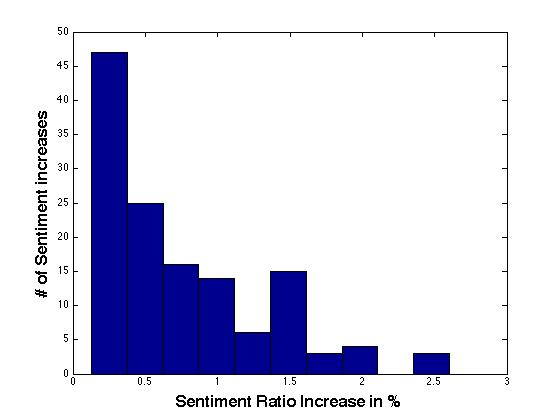
\includegraphics[width=\textwidth]{img/model/sentiment_increase}
                \caption{Price Increase Distribution of Sentiment Ratio}
                \label{fig:inc_dist}
        \end{subfigure}%
        ~ %add desired spacing between images, e. g. ~, \quad, \qquad, \hfill etc.
          %(or a blank line to force the subfigure onto a new line)
        \begin{subfigure}[b]{0.5\textwidth}
                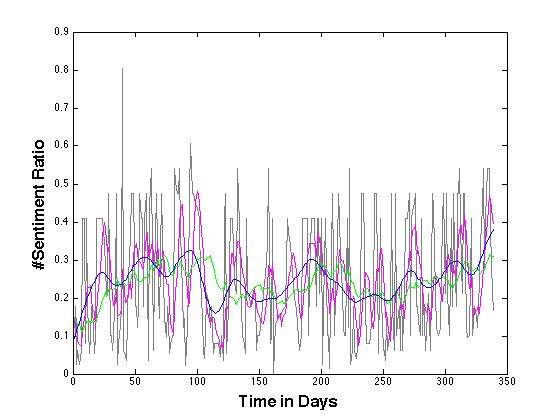
\includegraphics[width=\textwidth]{img/model/smoothing_variance}
                \caption{Comparison of Smoothing Functions}
                \label{fig:s_effect}
        \end{subfigure}
        ~ %add desired spacing between images, e. g. ~, \quad, \qquad, \hfill etc.
          %(or a blank line to force the subfigure onto a new line)

      
        \caption{Volatility of Social Media Features}\label{fig:distribution}
\end{figure}





\begin{table}[h]   
\centering
 \begin{tabular}{  c  | c  | c | c }
            
    \textbf{Smoothing}  & \textbf{S1 Product} & \textbf{S2 Subcategory} &\textbf{S5 Poverty} \\
  \hline 
  &&& \\
  No Smoothing & 0.1463*  &   0.1340* &    0.1719**  \\
  
  Weekly MA &    0.2528***   & 0.1830** &   0.3111***\\

  Monthly MA &  0.2889***  & 0.1466* & 0.4847*** \\

  HPD &  0.3586 ***  &  0.2673*** &   0.5957***  \\
  

\hline 

\multicolumn{4}{c}{\null}\\

\multicolumn{4}{c}{\textbf{Significance:} p $<$ .0005 ***, p $<$ 0.005 **, p $<$ 0.05 *}\\
\hline  

\end{tabular}
\caption{Sentiment Correlation}
\label{tab:smoothing_corr}


\end{table}


We further investigated to what extent Twitter lags as an indicator. Heaven Kwak showed that Twitter can bee seen similar to CCTV providers as a media for news where in some instances Twitter shoed to be ahead of life broadcasting shows such as CNN \cite{Kwak10}. If a casual relationship exists, how fast do prices react to Twitter conversations? Graphically this corresponds to shifting the sentiment ratio to the left. For each social media feature (51) we measured the correlation between one day and three days lag similar to \cite{Si_exploitingtopic}. We choose a window of three days because  none of the attention spikes showed to last longer than three days (Section 4.4). Furthermore it has been shown  that most trending topics only last for maximum seven days \cite{Kwak10}. The experiment was performed on all three commodities. In case of a disagreement, we solved the tie through a majority voting. A lag of three days clearly favoured the correlation with 44 out of 51 (0.86 \%) features and a one day lag for 7 out of 51 (14 \%) features. 



\subsection{Price Model Results}

The prediction results across different time horizons are highlighted in Figure \ref{fig:res_1}. These results are obtained using the model described in Section \ref{5.5} with the top 10 features obtained through the feature selection procedure explained in the previous section. The features used in the form of $y_{t-2}$ are the top 10 obtained from the feature selection process. 
 Looking at the results ANFIS performs exceptionally well for day to day predictions and as expected decreases its performance as the horizon increases. The commodity beef seems to be the easiest prediction task and further analysis will clearly show why.   We observe that RMSE linearly increases over the period until prediction horizon 20. Prediction accuracy rapidly decreases and becomes unstable from then onwards. To analyse the results in more detail and to put the RMSE into context  we turn our attention towards Figure \ref{fig:wheat_1} \ref{fig:beef_1} \ref{fig:milk_1}. For all three commodities, the predictions within one week are accurate. We can now also observe why beef had the lowest RMSE among the three commodities. Beef follows a clear upwards trend. Such long lasting motions are much easier to predict and as discussed in Section \ref{featSel_bench} our input variables from the intermediate past are descriptive if there is a clear underlying motion. 
For the model $y_{t+20}$  ANFIS clearly overestimates a decrease and increase in price but still manages to captures the underlining trend. The overestimation seen in Figure \ref{fig:long_wheat_price} and Figure \ref{fig:long_milk_price} strongly approximates the observed pattern in the training sample explaining the deviation from the actual prediction. The only commodity excluded from this behaviour is beef due to its strong underlying motion. 





\begin{figure}[H]
        \centering
         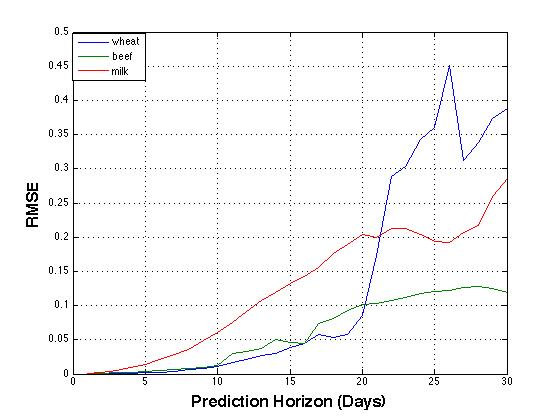
\includegraphics[width=.66\textwidth ]{img/model/prediction_days_1}      
        \caption{Prediction Accuracy - Benchmark }
        \label{fig:res_1}
\end{figure}




\begin{figure}
        \centering
        \begin{subfigure}[b]{0.5\textwidth}
                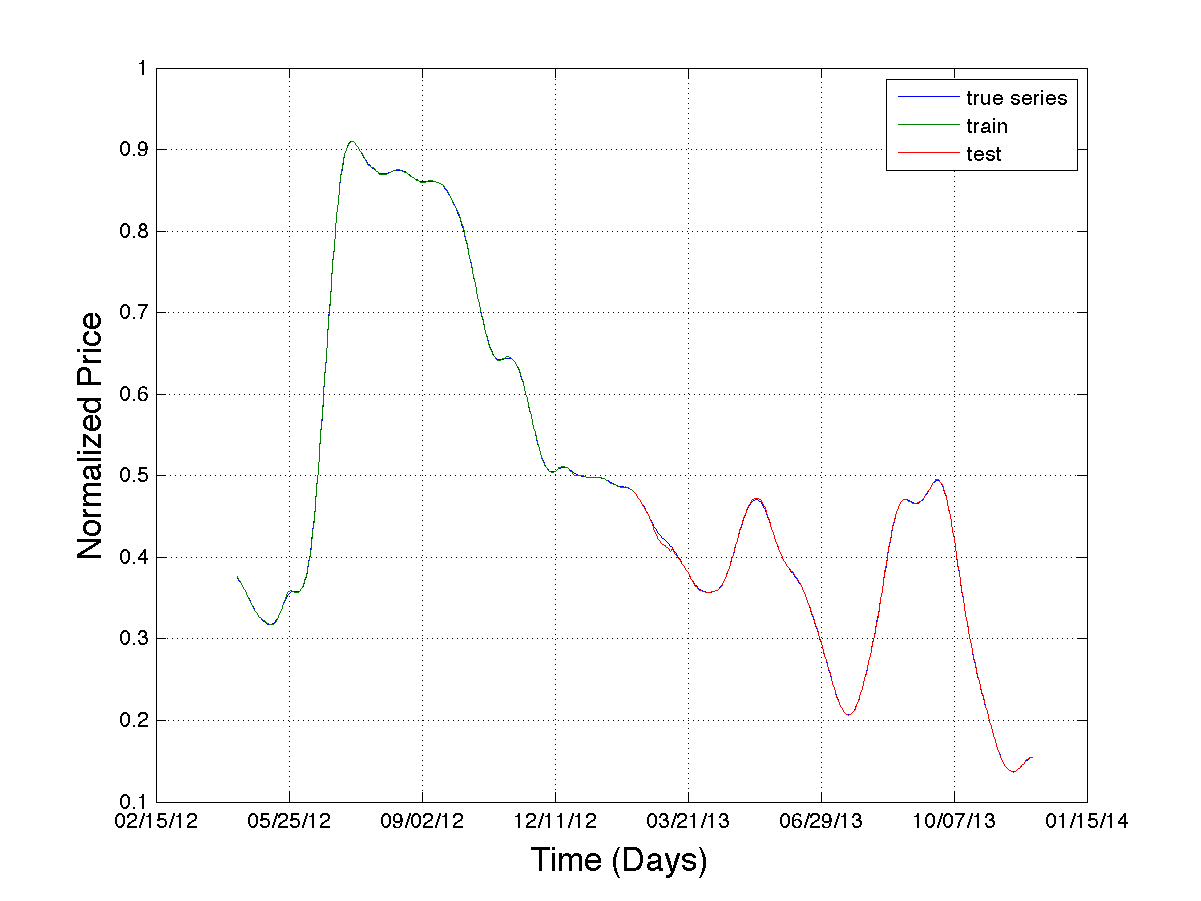
\includegraphics[width=\textwidth]{img/model/wheat/model1/pred_4}
                \caption{4 Day Horizon - RMSE 0.0015948 }
                \label{fig:gull}
        \end{subfigure}%
        \begin{subfigure}[b]{0.5\textwidth}
                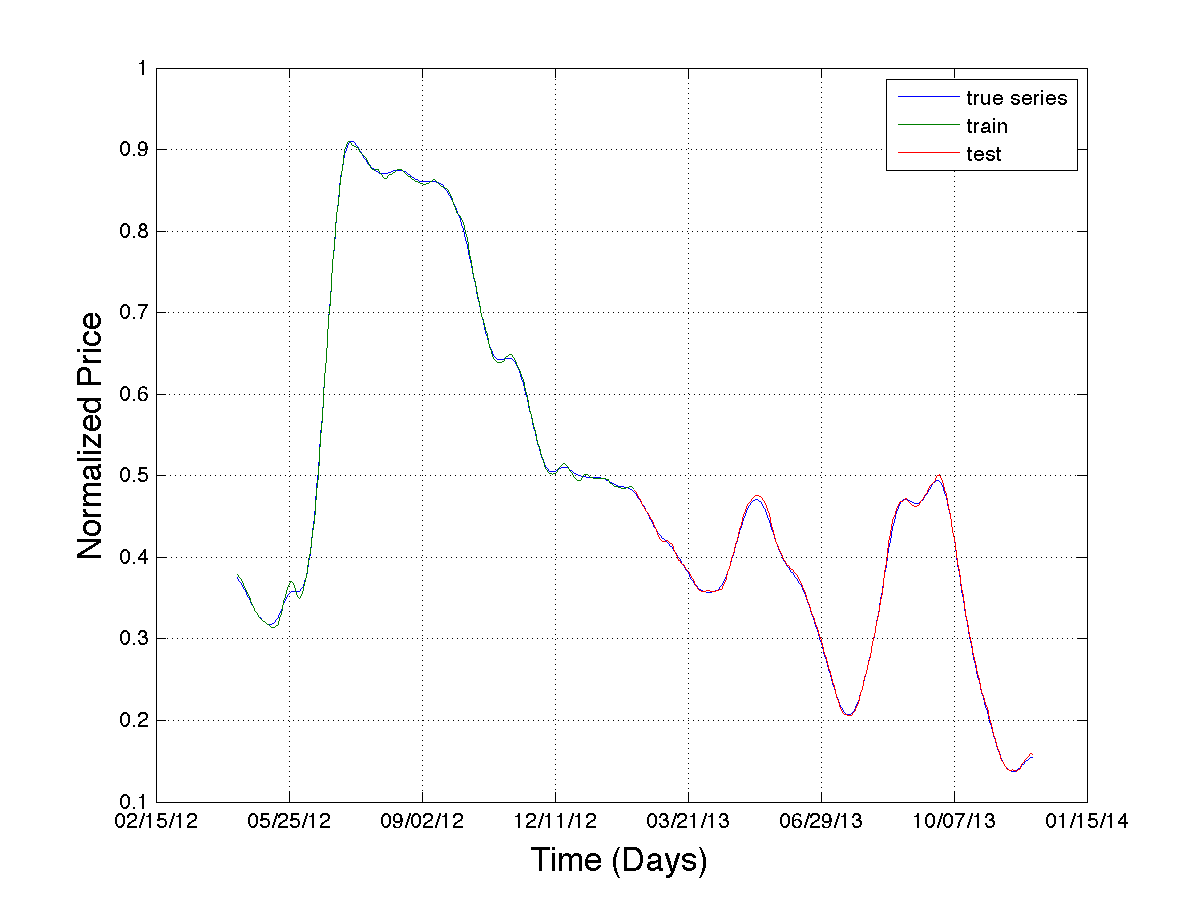
\includegraphics[width=\textwidth]{img/model/wheat/model1/pred_7}
                \caption{7 Day Horizon - RMSE 0.0030423}
                \label{fig:tiger}
        \end{subfigure}
       
       \hfill
       
        \begin{subfigure}[b]{0.5\textwidth}
                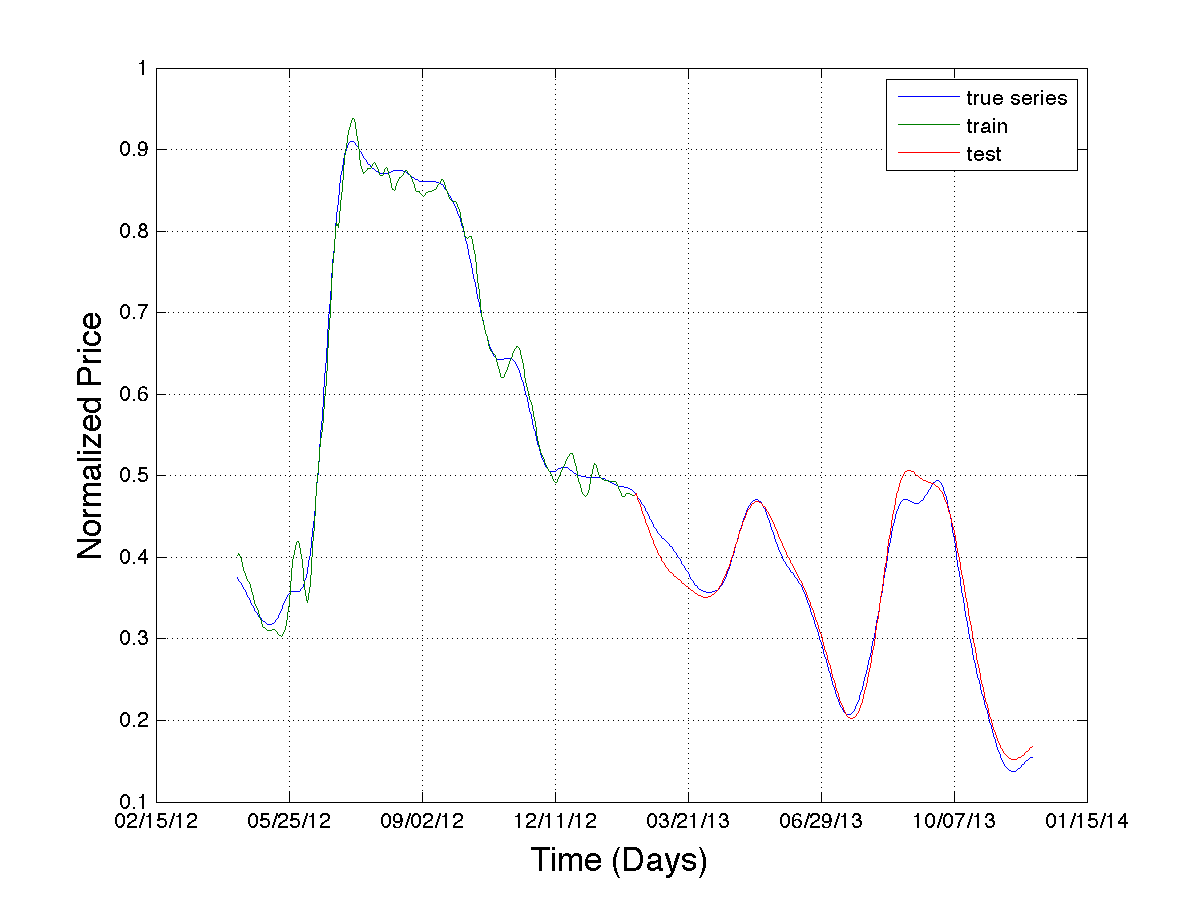
\includegraphics[width=\textwidth]{img/model/wheat/model1/pred_14}
                \caption{14 Day Horizon - RMSE 0.015192}
                \label{fig:mouse}
        \end{subfigure}%
         \begin{subfigure}[b]{0.5\textwidth}
                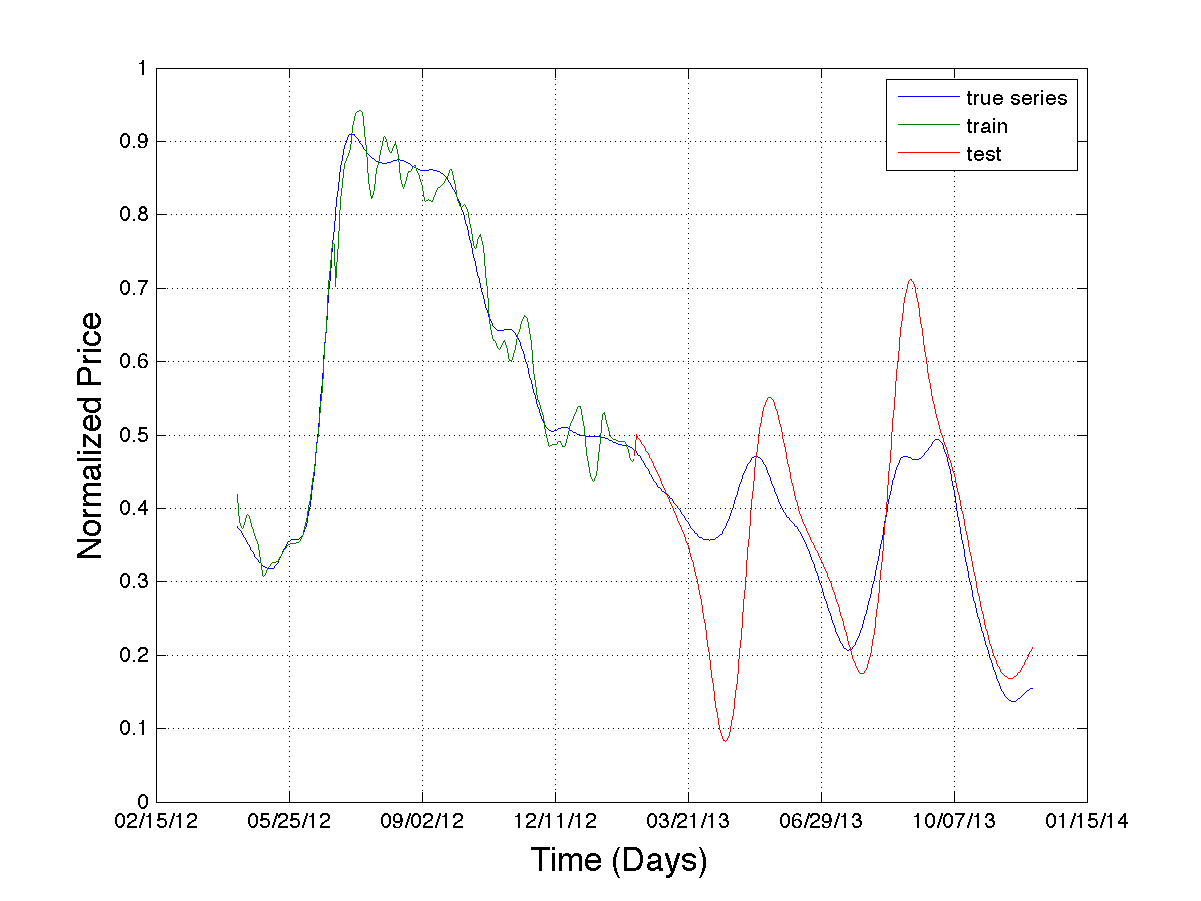
\includegraphics[width=\textwidth]{img/model/wheat/model1/pred_21}
                \caption{21 Day Horizon - RMSE  0.105}
                \label{fig:long_wheat_price}
        \end{subfigure}
        \caption{Benchmark Prediction Wheat}
        \label{fig:wheat_1}
               
\end{figure}





\begin{figure}
        \centering
        \begin{subfigure}[b]{0.5\textwidth}
                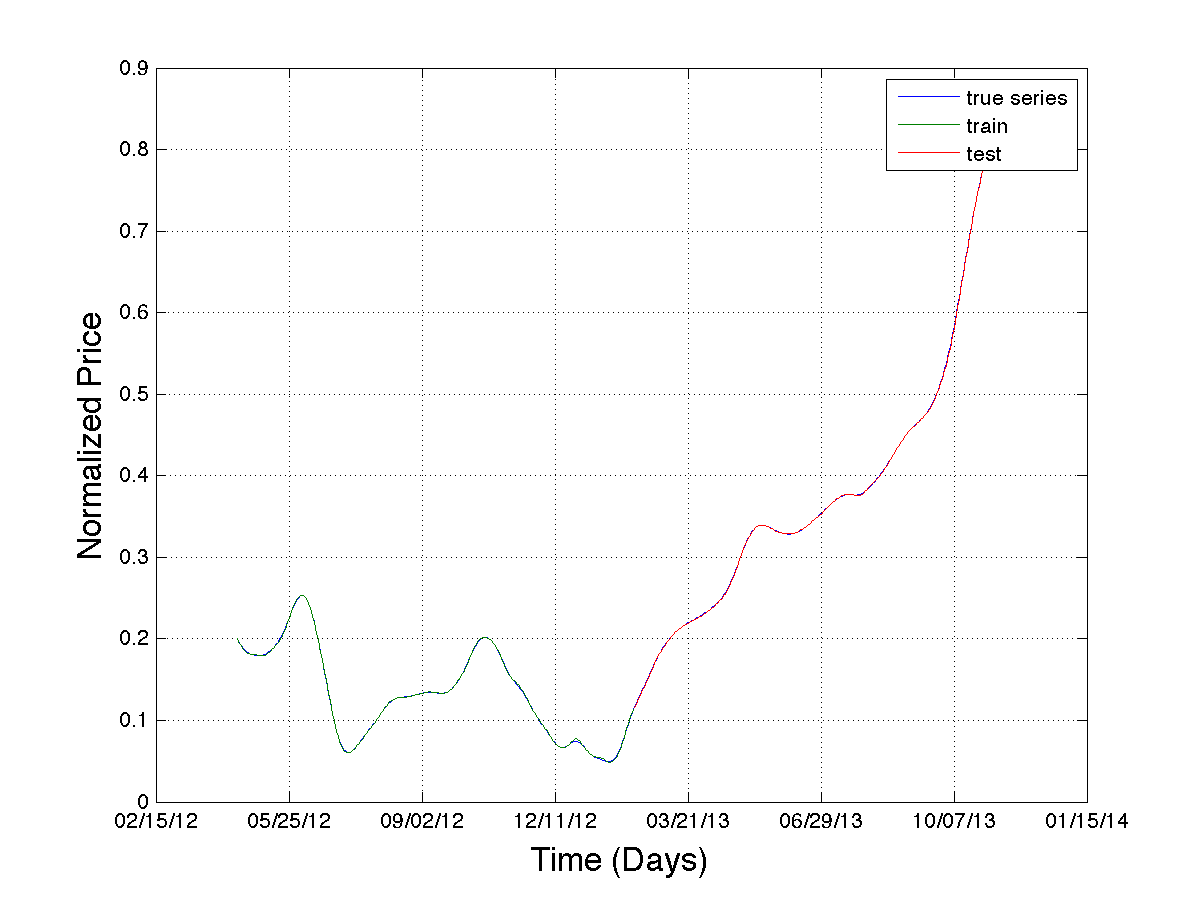
\includegraphics[width=\textwidth]{img/model/beef/model1/pred_4}
                \caption{4 Day Horizon - RMSE 0.00086578 }
                \label{fig:gull}
        \end{subfigure}%
        \begin{subfigure}[b]{0.5\textwidth}
                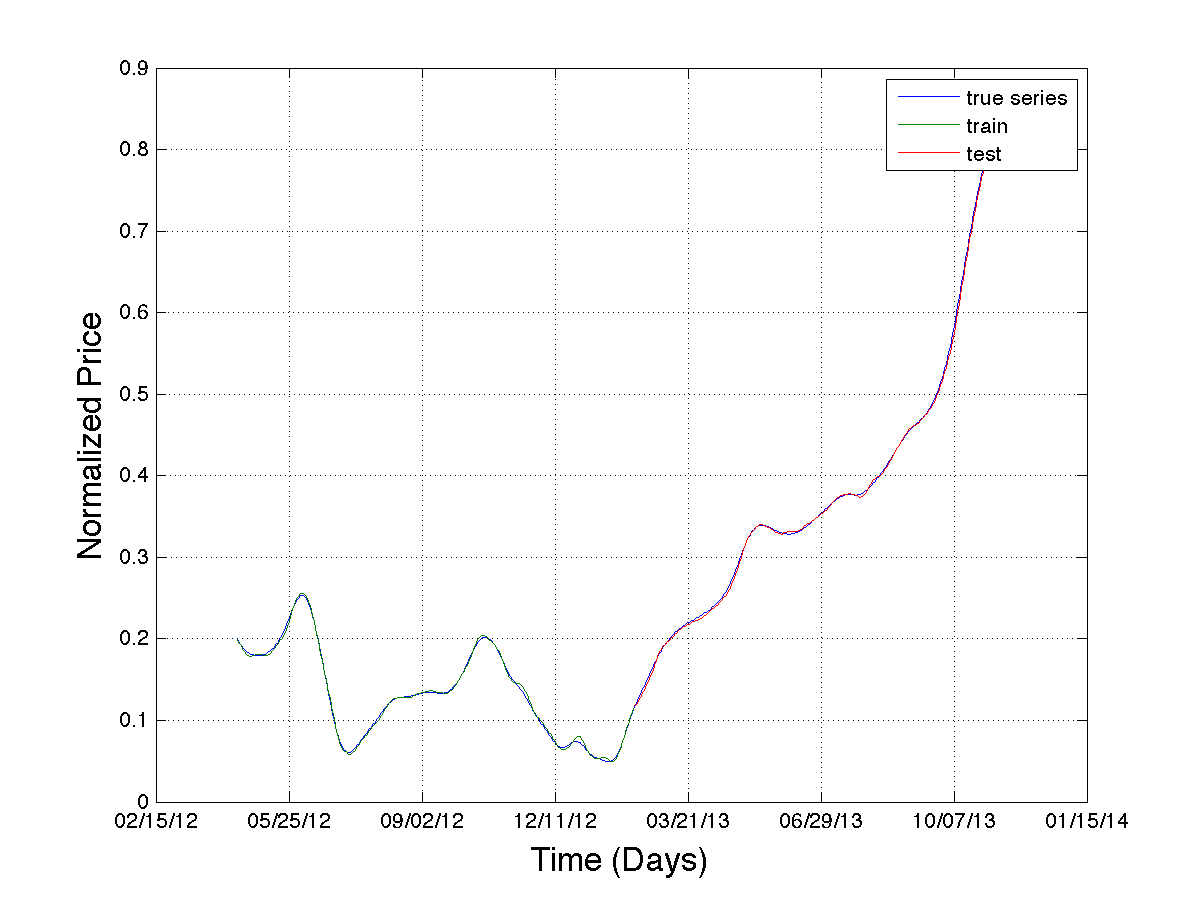
\includegraphics[width=\textwidth]{img/model/beef/model1/pred_7}
                \caption{7 Day Horizon - RMSE 0.0059255}
                \label{fig:tiger}
        \end{subfigure}
       
       \hfill
       
        \begin{subfigure}[b]{0.5\textwidth}
                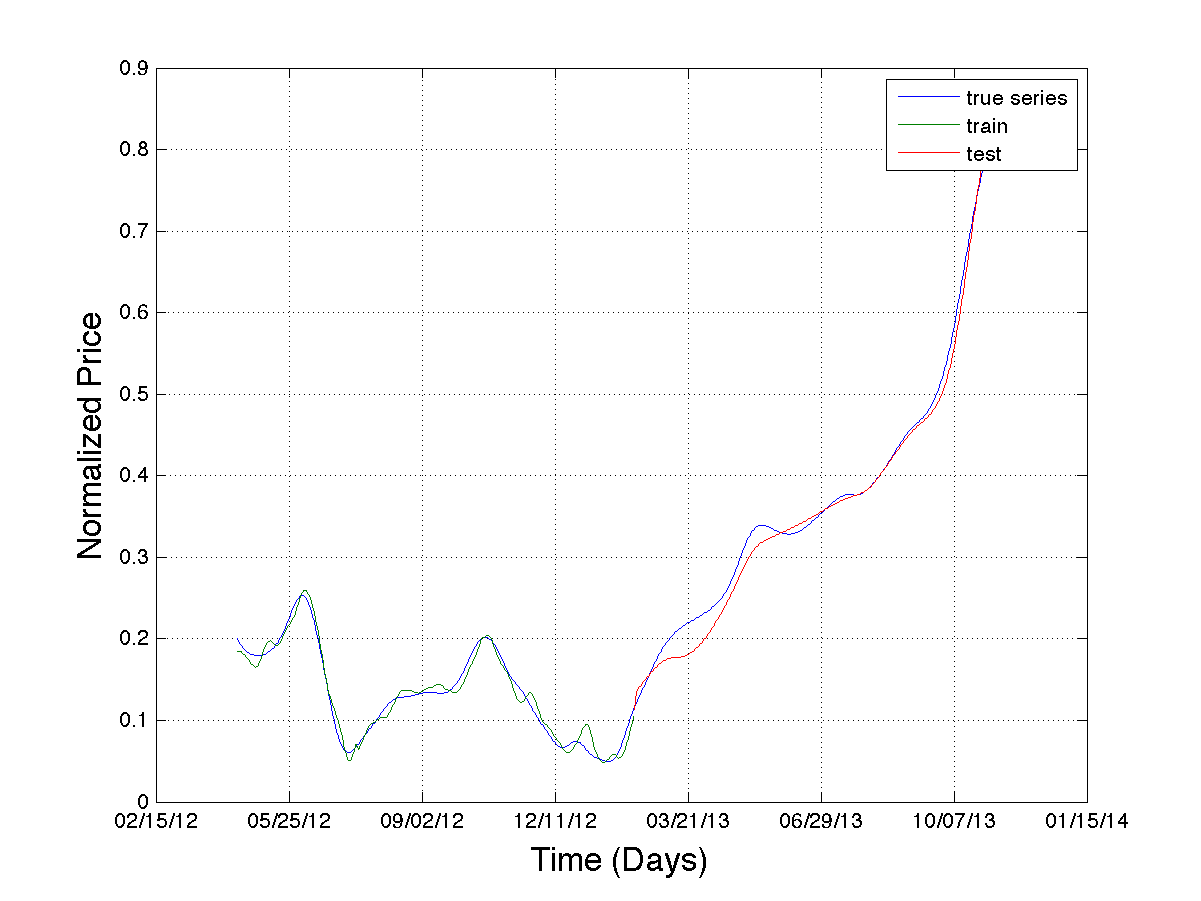
\includegraphics[width=\textwidth]{img/model/beef/model1/pred_14}
                \caption{14 Day Horizon - RMSE 0.017041}
                \label{fig:mouse}
        \end{subfigure}%
         \begin{subfigure}[b]{0.5\textwidth}
                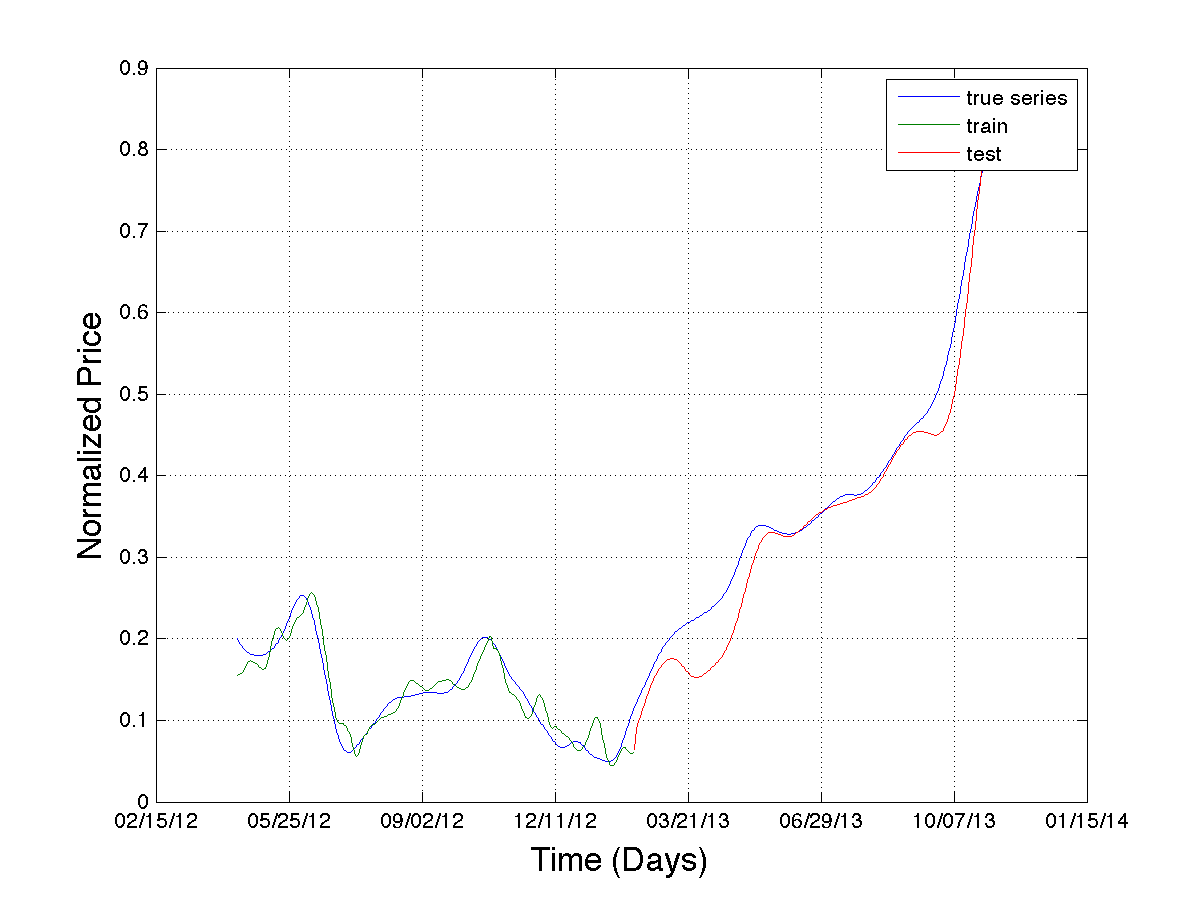
\includegraphics[width=\textwidth]{img/model/beef/model1/pred_21}
                \caption{21 Day Horizon - RMSE 0.040397}
                \label{fig:mouse}
        \end{subfigure}
        \caption{Benchmark Prediction Beef}
        \label{fig:beef_1}
\end{figure}




\begin{figure}
        \centering
        \begin{subfigure}[b]{0.5\textwidth}
                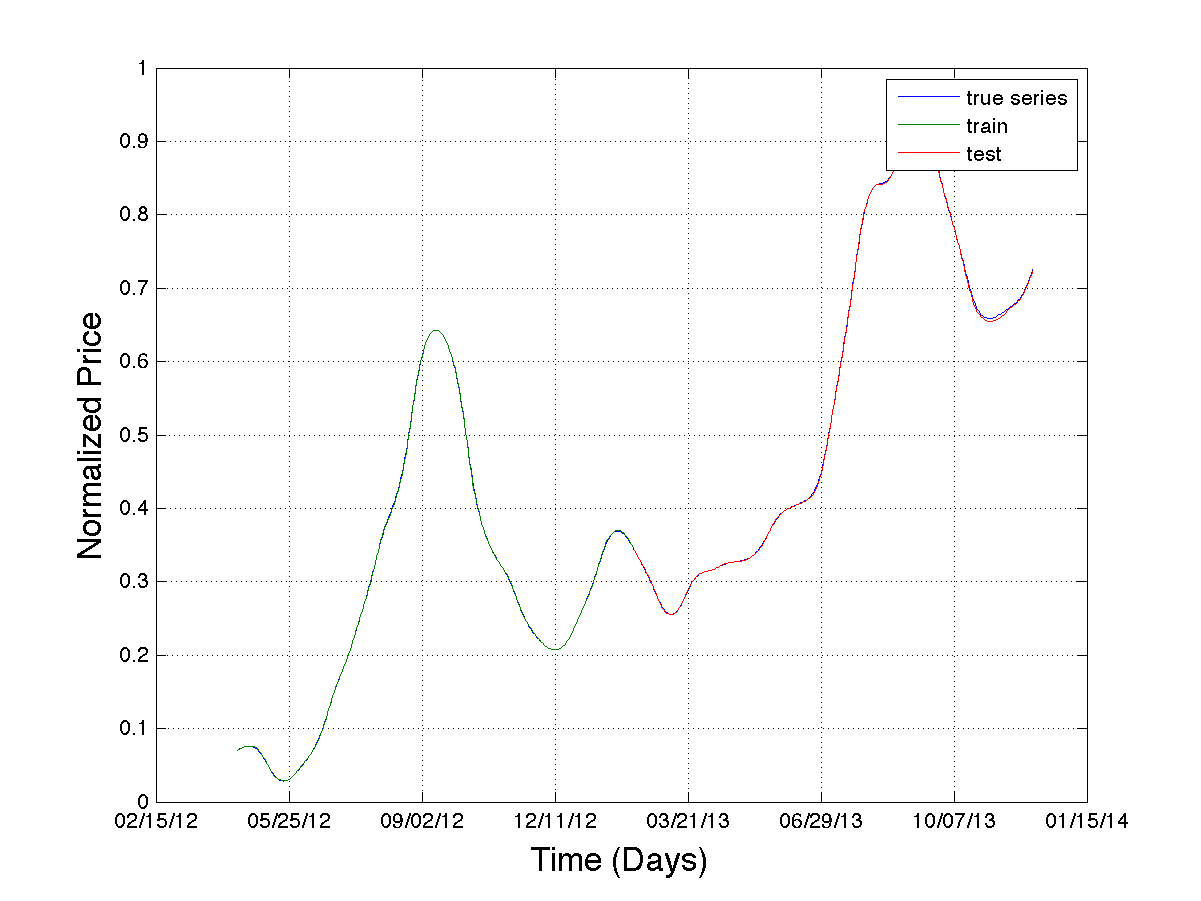
\includegraphics[width=\textwidth]{img/model/milk/model1/pred_4}
                \caption{4 Day Horizon - RMSE 0.0015964}
                \label{fig:gull}
        \end{subfigure}%
        \begin{subfigure}[b]{0.5\textwidth}
                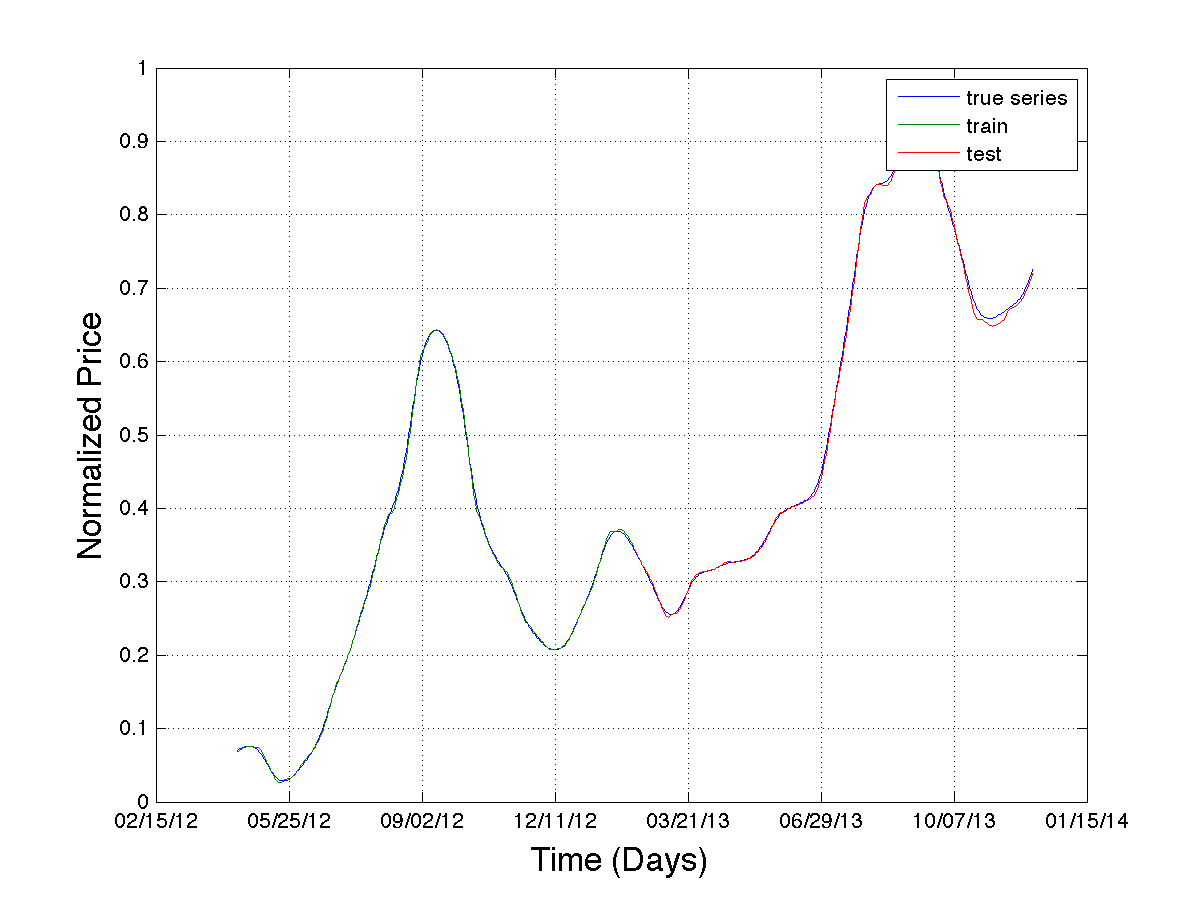
\includegraphics[width=\textwidth]{img/model/milk/model1/pred_7}
                \caption{7 Day Horizon - RMSE 0.0049564 }
                \label{fig:tiger}
        \end{subfigure}
       
       \hfill
       
        \begin{subfigure}[b]{0.5\textwidth}
                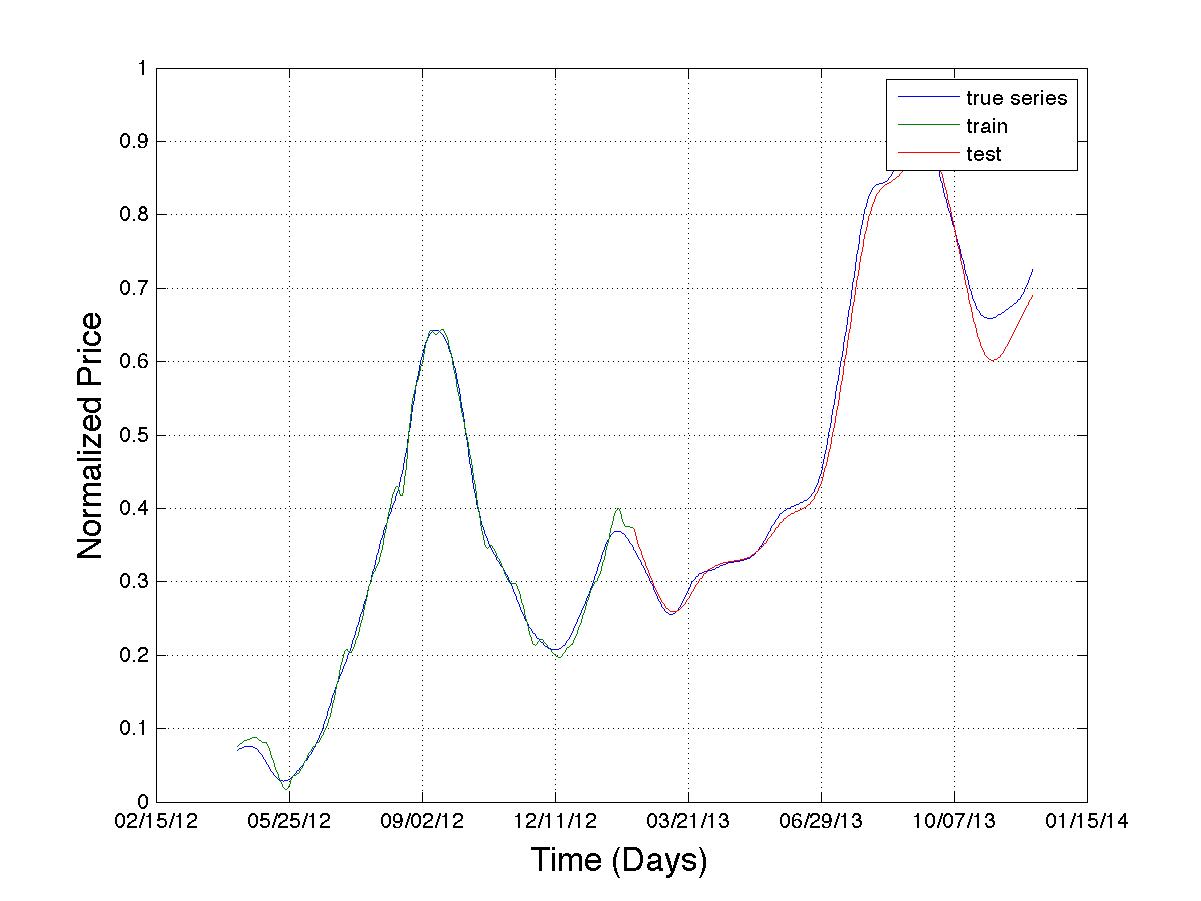
\includegraphics[width=\textwidth]{img/model/milk/model1/pred_14}
                \caption{14 Day Horizon - RMSE 0.1185}
                \label{fig:mouse}
        \end{subfigure}%
         \begin{subfigure}[b]{0.5\textwidth}
                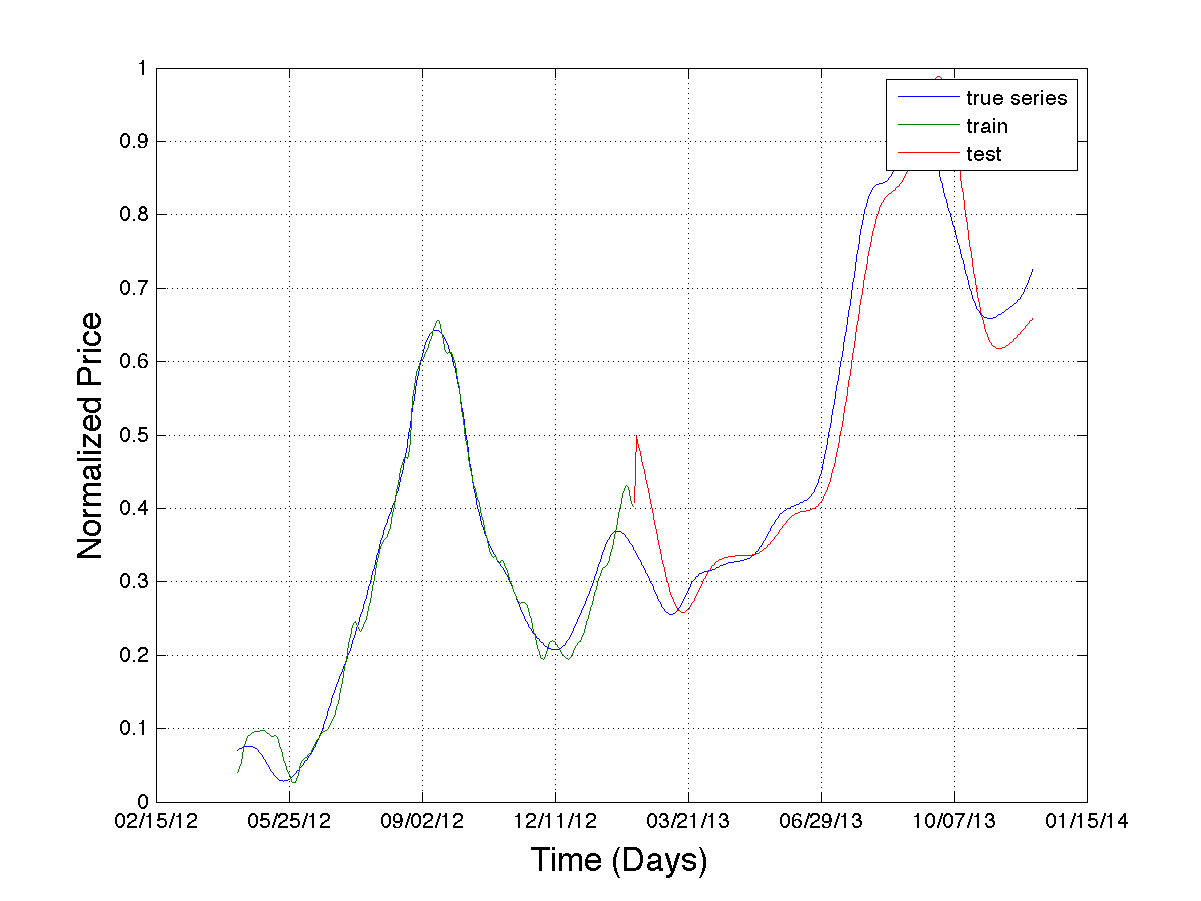
\includegraphics[width=\textwidth]{img/model/milk/model1/pred_21}
                \caption{21 Day Horizon - RMSE 0.023702}
                \label{fig:long_milk_price}
        \end{subfigure}
        \caption{Benchmark Prediction Milk}
        \label{fig:milk_1}
\end{figure}







\subsection{Social Media Model Evaluation}
\label{result_m2}

Unlike our benchmark paradigm, the social media model did not exhibit an increasing error rate with increasing horizon. We hence focused our attention on analysing day to day predictions. From Figure \ref{fig:social_results} it is apparent that our strengthening attempts have improved the prediction accuracy across all commodities. However, there is a clear difference in the quality of the predictions between the three commodities. For wheat, we were able to follow the real price line, not so for milk. Why does the prediction model favour the commodity wheat? Our first attempt was to investigate the linear relationship between the features and the price. The correlation analysis favoured the commodity milk however the difference is negligible. Our second intuition was to check whether the training data generalises well for the entire data set. We observed that the training and test dataset exhibited different behaviours. More specifically we found that certain features showed a negative correlation in the train set, however, a positive relationship in the test set. We experimented with various sizes of train sets but none of them notably improved the prediction results. Lastly, we were motivated to examine the content of the Tweets. The set of wheat Tweets might be more relevant to our given topic then the set of milk Tweets. For the purpose of this analysis, we computed the 10 most occurring nouns of the Tweets containing at least one term of the subcategory wheat, beef or milk along the 10 most frequently occurring bigrams. We use the number of keywords as a proxy of the overall number of tweets. This approach has limitations as we can not account for  Tweets that contain more then one frequent term. For each of the frequent nouns we manually investigated the tweets to asses if the keyword captures relevant Tweets. Incase of ambuguity we considered the bigrams to help us point to the right context. If the bigram pointed towards a relevant product we accepted the term as relevant else we subtracted the occurrence count of irrelevant bigram from the total count of the ambigious term and accepted the remaining count as relevant. Furthermore we added the count of the irrelevant bigram to the total count of irrelevant terms. Consider the example of cream with a total keyword count of 1000. The bigram of ice cream occurs 600 times. We hence subtract the 600 from the 1000 and count 400 keywords as relevant and 600 as irrelevant. Following this approach we tried to quantify the entropy of our tweet. We did this analysis for the conversations centred around price, supply and poverty as the features crafted from these topics constitute the majority in our model. Notably, across all conversation topics, the discussions centred around wheat showed the highest relevance (i.e. the number of keywords retrieved  deemed relevant was higher). Examples of accepted term counts were \emph{bread, pasta, noodles and flour}. One of the only terms we rejected was \emph{gluten}. The bigram pointed to the context of \emph{gluten free} which is clearly not what we try to capture. Overall we approximate a value of 88 \%  of the tweets being relevant for the discussion centered around wheat. For beef frequently accepted terms were \emph{beef, steak, cattle cow and meat}. A subset of words deemed irrelevant were \emph{bitches} and \emph{chicken}. Beef is used in urban language as \emph{to have a grudge agains somebody} which is why often the term \emph{beef} and \emph{bitch} were present in the same tweet. One of the bigrams pointed us to \emph{chicken steak}. Such tweets off topic. In total we approximated 84 \% of the tweets of being relevant. 
Lastly we performed the experiment for the commodity milk. The only terms we marked as unambiguous were \emph{milk} and \emph{wheat}. The bigram containing the word cream showed that most of the conversation was centered around \emph{ice cream}. Due to its distance relationship we consider this set of words as unrelated. Similarly for butter we observed that most of the tweets containing the word were referring to peanut butter. Again we considere the set of tweets containing peanut butter as irrelevant. Further terms that lead to irrlevant tweets were \emph{cake, yogurt}. For milk we only observed a relevance of 60 \%.  On the basis of these findings, we conclude that the list of keywords used for milk retained a high number of Tweets that were not relevant,  highly impacting the quality of the predictions. 

We further investigate if we could determine a clear relationship between the features of wheat and the predicted outcome. The only variable that showed some describable relationship was the sentiment ratio of poverty. We calculate the sentiment ratio as \#positive / \#negative. It follows that with an increase of negative sentiment the price drops and rises as the ratio of positive sentiment increases. 


 A visual analysis 






\begin{figure}[H]
        \centering
        \begin{subfigure}[b]{0.5\textwidth}
                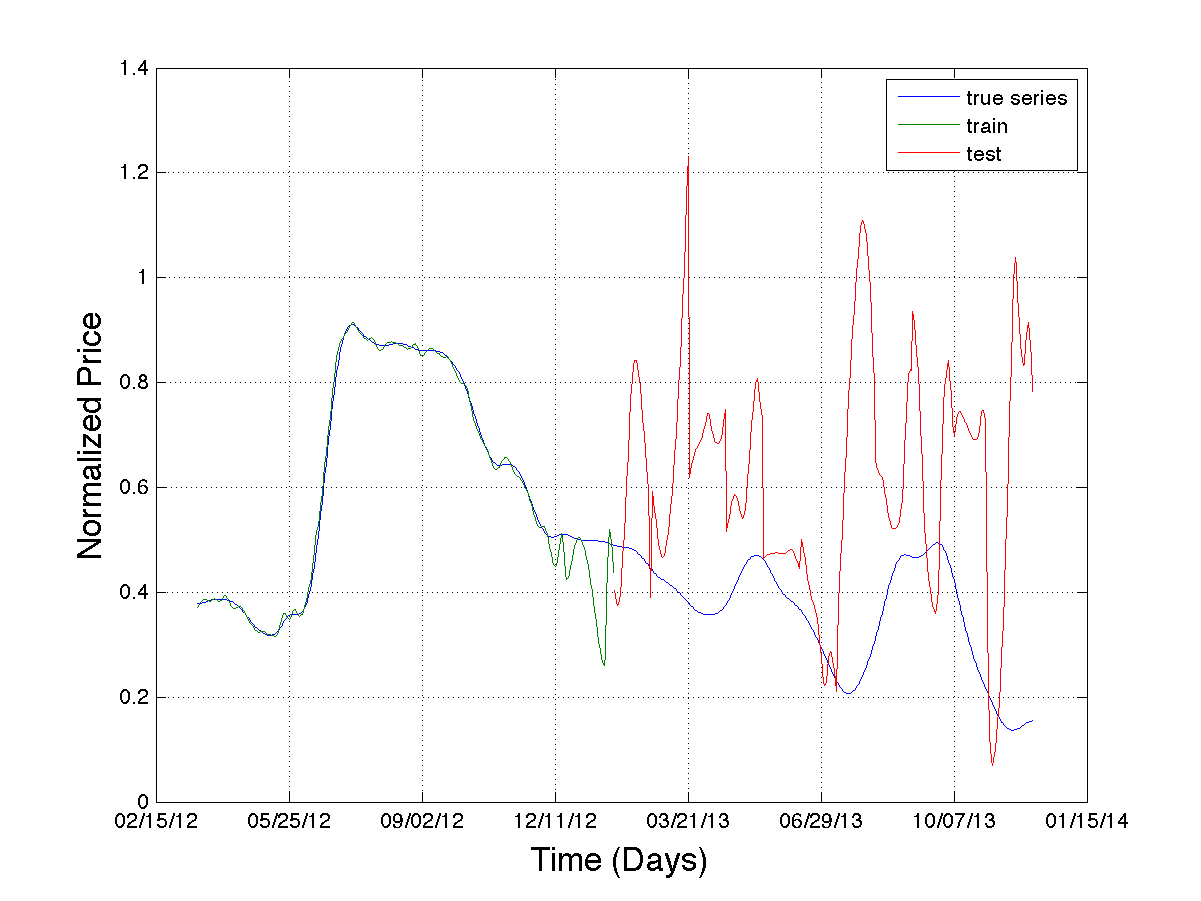
\includegraphics[width=\textwidth]{img/model/exp2/wheat/pred_1}
                \caption{1 Day Horizon Wheat - RMSE 0.3580}
                \label{fig:gull}
        \end{subfigure}%
           \begin{subfigure}[b]{0.5\textwidth}
                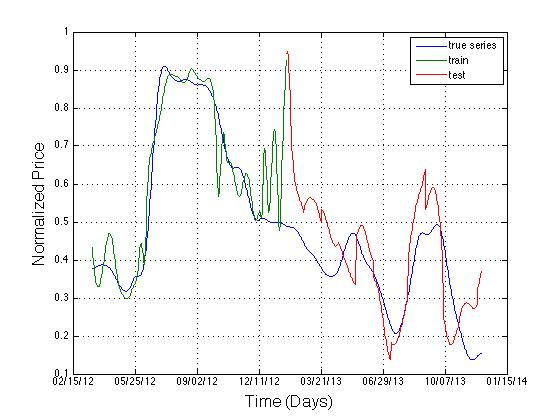
\includegraphics[width=\textwidth]{img/model/exp2_final/wheat_1}
                \caption{1 Day Horizon Wheat - RMSE 0.1083}
                \label{fig:gull}
        \end{subfigure}%
              \hfill    
        \begin{subfigure}[b]{0.5\textwidth}
                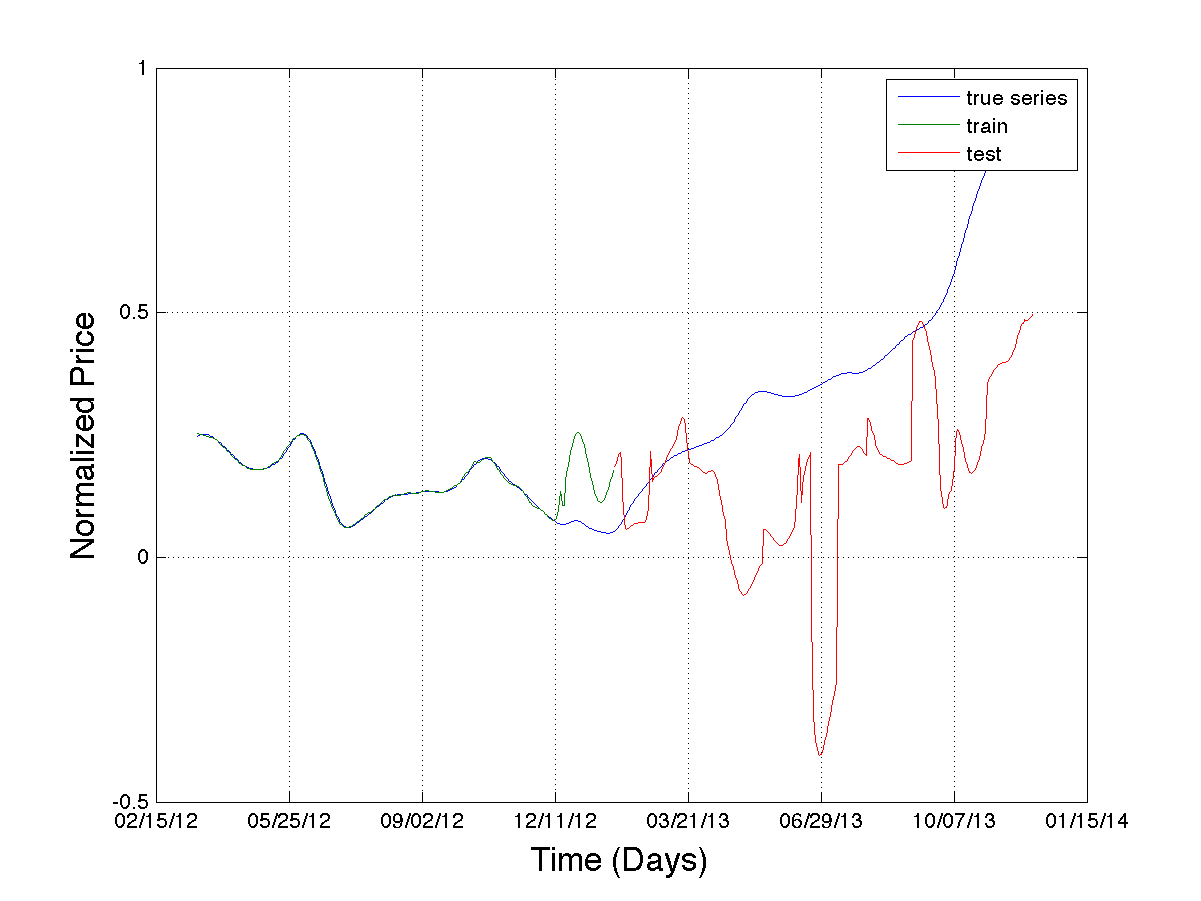
\includegraphics[width=\textwidth]{img/model/exp2/beef/pred_1}
                \caption{1 Day Horizon Beef - RMSE 0.3209  }
                \label{fig:tiger}
        \end{subfigure}%
              \begin{subfigure}[b]{0.5\textwidth}
                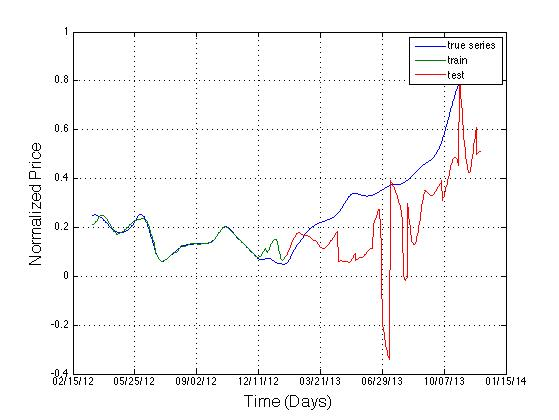
\includegraphics[width=\textwidth]{img/model/exp2_final/beef_1}
                \caption{1 Day Horizon Beef  - RMSE 0.2383 }
                \label{fig:tiger}
        \end{subfigure}%
        \end{figure}
        
        \begin{figure}[H]
        \centering
        \begin{subfigure}[b]{0.5\textwidth}
                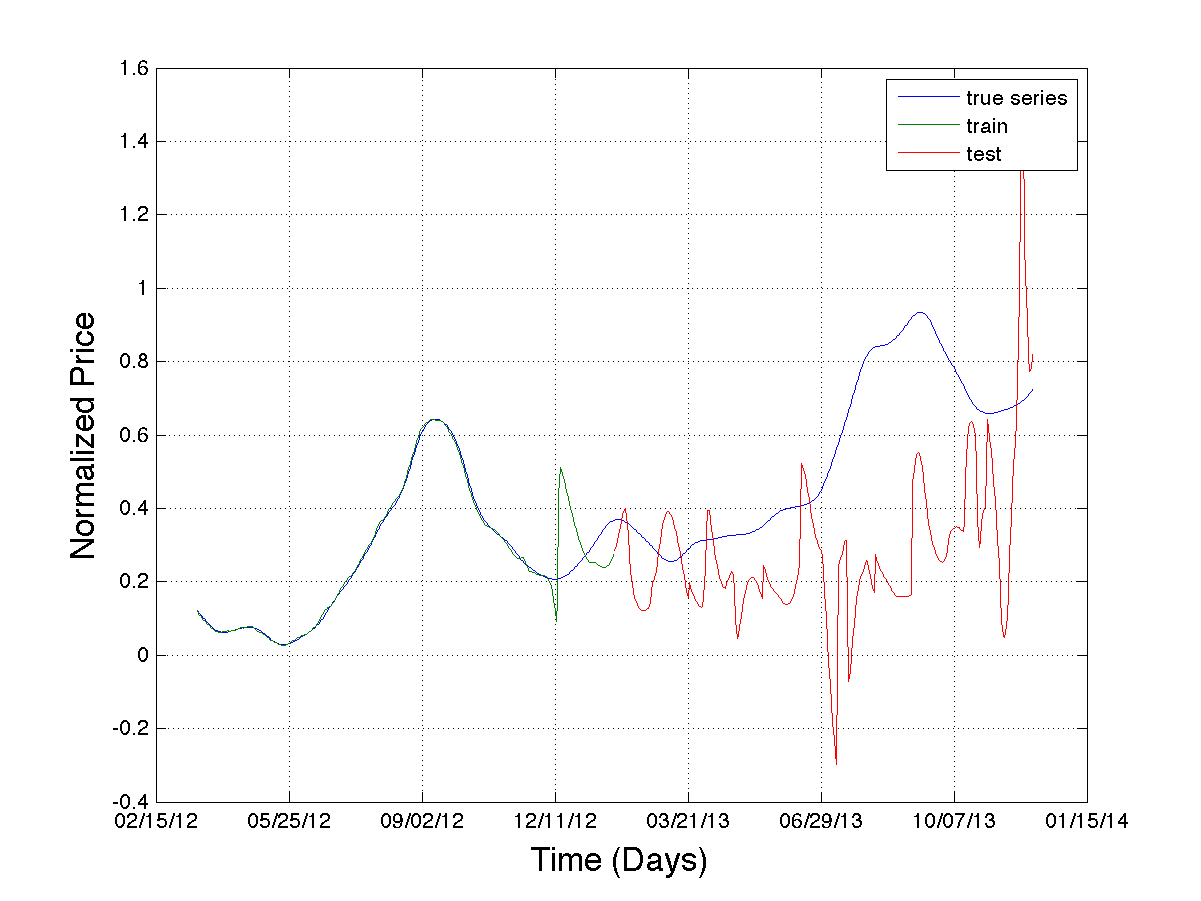
\includegraphics[width=\textwidth]{img/model/exp2/milk/pred_1}
                \caption{1 Day Horizon Milk- RMSE 0.3782}
                \label{fig:mouse}
        \end{subfigure}%
            \begin{subfigure}[b]{0.5\textwidth}
                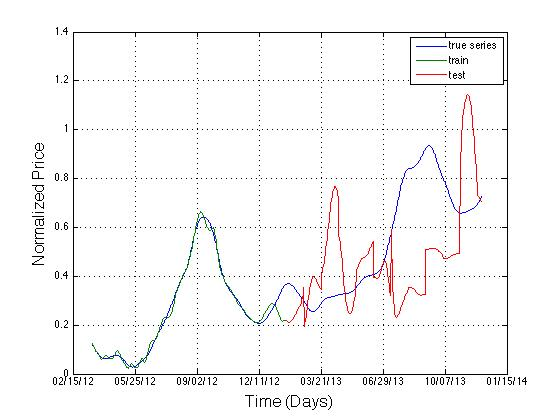
\includegraphics[width=\textwidth]{img/model/exp2_final/milk_1}
                \caption{1 Day Horizon Milk - RMSE  0.2960}
                \label{fig:mouse}
        \end{subfigure}%
    
    
        \caption{Social Media Prediction}\label{fig:social_results}
\end{figure}






\subsection{Mixture Model}
\label{final_result}


As our mixture model exhibits similar behaviours to the price model, we show the exact predictions for each commodity in the Appendix \ref{ts_model}. Instead we focus our attention on the performance comparison of the three different models (e.g. price, social and mixture model). Figure \ref{fig:final_res} summarises our results and compares the three models. For all commodities, the social media model performs rather badly. We can hence conclude that a model solely based on social media feature will yield no accurate predictions.  From the wheat forecasts we can see that both the mixture and price model have comparable results. Across all horizons, we recorded an average error of 0.0669 for the price model and an average error of 0.07315808 for the mixture model. It seems like the price models favour the intermediate future whereas the mixture model allows for more accurate predictions in the far foresight. To test this hypothesis we extended the analysis to $y_{t+50}$, however, rejected it as we could not record any clear performance improvements compared to the price model.  

Similar patterns apply to the commodity beef. Since beef exhibits a strong and long lasting trend, the prediction accuracy is high for both models and a difference is hardly observable. At the end of the prediction horizon, the mixture model performs slightly better. For the price model, we observe an average error of 0.02816 whereas for the mixture model an error of 0.02814. For the commodity milk, the price predictions are clearly more accurate than the ones of the mixture model. This is attributed to the social media's high-level of noise and a lack of focus that we observed for the commodity milk.  

\subsection{General comments to the Results}


We started our evaluation with defining three input models for a time series prediction based on historical price data, social media features and lastly a mixture model. Our general observation was that only our price model allowed to generalise well over over different commodities  and price horizons. Social media features were shown to be more specific to a specific commodities. The model selection process clearly favoured sentiment meassures over contextually sensitive tweets and raw volume. Similar for the mixture model the feature selection process resulted with a different set of features for each commodity and likewise favoured sentiment over twitter attention. Through our quantitative and qualitative analysis we clearly showed that an increase in twitter volume is not due to an increase in price. 

 %A commonality observed between the pure models and the mixture model was that popular features in the pure models were reflected in the mixture model. I.e. we observe features from the intermediate past to be both present in the price model and mixture model and likewise sentiment features taking the majority in social media model and in the mixture model.
 
  %From our analysis in Section \ref{corr_results} it is not surprising that hardly any features based on volume count were considered. John Bollen however found a nonlinear relationship between the count of tweet and the stock market which we could not confirm for the case of commodity prices using our specific setting. 
  
  A last observation we make regarding the input model is that prices that follow a clear trend during a long period of time  favour features crafted from historical price data where as commodities that follow a price trend that is nonlinear prefer social media features crafted from sentiment. The later can be explained by Robert Marx's theory that intermediate historical data features based on the intermediate past are predictive for prices characterised through long lasting motions. 

For our concrete prediction we used the price model as a baseline. First experiments with the social media model failed to follow the price line which is why we experimented with different signal soothing techniques. Or conclusion was that a higher smoothing factor favoured future predictions which is not surprising as compared to the price data twitter volume and sentiment are characterised by a much higher day to day volatility. Twitter has been found to propagate news in some instances ahead of broadcasting channels such as CNN. We hence determined a lag factor between the twitter data and the commodity price data. We found that a lag of 3 days favoured the predictions. 

Despite our efforts of strengthening the social media features predictions sole based on  the social media input model were considerably less accurate then the ones achieved by the baseline. Our initial hypothesis was that daily twitter conversations fluctuates within a well defined baseline and that a sudden rise will be due to a strong increase in price. Although the increase in twitter volume could be attributed to events most of them have been found to be off topic. Nontheless we found that for the commodity wheat a decrease in negative sentiment lead to an increase in price. in other words twitters users seem to be happy when the prices for commodity increase. However we were unable to genearlise this claim among other commodities.
 
 A stricter keyword selection procedure in Section \ref{red_lex} might migate this problem but could also lead to excluding informative tweets. It is a trade-off that requires further attention. The problem of irrelevant tweets is further fueld by Twitter's gain in popularity. More often then not false event were caused by online celebrities. Such users are usually characterised by a high follower count causing a non-linear effect through a high number of retweets \ref{}. Considering twitter meta data might help to distinguish spammers from trustworthy sources. Our experiments showed that the relevance or the entropy of the tweets highly affect the prediction accuracy. However for applying stricter filtering mechanisms we will need more relevant data. The key is relvance. We don't believe that more time series will help the model learn relevant patterns. We initially assumed that a larger training set would improve the accuracy. However our experiments showed that with growing training set the predictions did not increase in accuracy. We assume that older data loses its relevance to future predictions. Hence the above motivated optimisation steps will only be helpful if further datasources can be consdered. We propose to specially daggregate the analysis to countries that are more sensitive towards price data. We are comfident that this would allow for more robust models and help generalise claims. 
 
Although our social media features did not deliver the predictive power we were hoping for we still believe that coupled with price data it should be the preferred choice over a homogen price model. 
 
 
 We believe that the
highest improvements in our thesis can be gained from identifying and removing spam


 We believe exlcluding Identifying trusty users
Are qualitative analysis showed that our sample is prune by noise. 

made similar observations regarding prices with long lasting trends and conluded that 


 From a proposed set of 33 price features we found the variables in the intermediate past to be most desricriptive of the price variance. 


To improve the overall predictions we experimented with different segmentation of the training data (50 \% , 70 \%, 85 \%) 






%wheat price : avg 0.0669  milk price : avg 0.04048 beef price : avg 0.028160 beef mix: avg 0.02814 milk mix: avg 0.09770191 wheat mix avg: 0.07315808



\begin{figure}
        \centering
        \begin{subfigure}[b]{0.5\textwidth}
                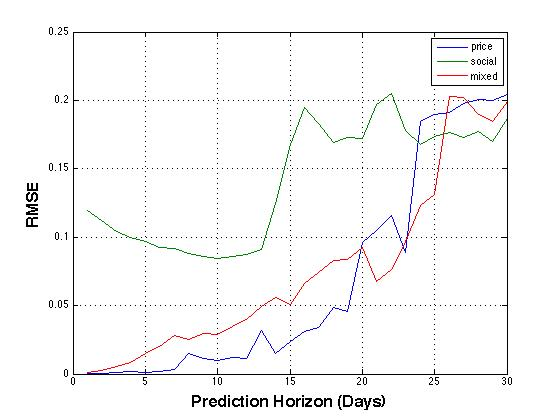
\includegraphics[width=\textwidth]{img/model/results/result_wheat}
                \caption{Model Comparison Wheat- RMSE 0.016061}
                \label{fig:gull}
        \end{subfigure}%
           \begin{subfigure}[b]{0.5\textwidth}
                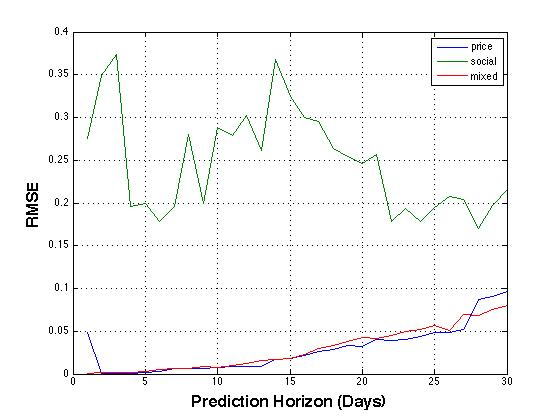
\includegraphics[width=\textwidth]{img/model/results/result_beef}
                \caption{7 Day Horizon Milk - RMSE 0.031539}
                \label{fig:gull}
        \end{subfigure}%
              \hfill    
        \begin{subfigure}[b]{0.5\textwidth}
                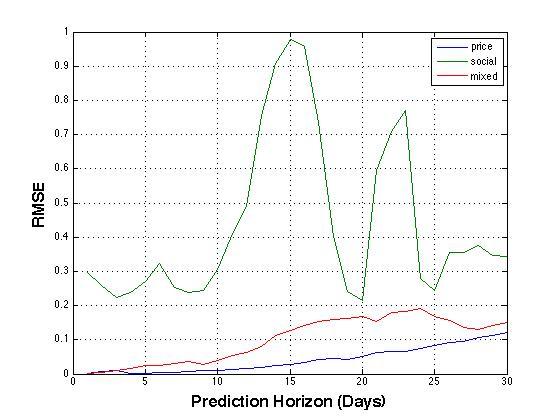
\includegraphics[width=\textwidth]{img/model/results/result_milk}
                \caption{14 Day Horizon Milk - RMSE 0.11321  }
                \label{fig:tiger}
         \end{subfigure}%
         
        \caption{Social Media Prediction}\label{fig:final_res}
\end{figure}







%%%%%%%%%%%%%%%%%%%%%%%%%%%%%%%%%%%%%%%%%%%%%%%%%%%%%%%%%%%%%%%




\begin{comment}

\subsection{Curse of of Dimensionality}

For Fuzzy interference systems there are generally three types of input space partitionings. We can classify them as grid, true and scattered portionin. We first applied grid pertaining which generates rules by enumerating all possible combinations of membership functions. However for three membership functions and x features this leads to $3^x$ possible combinations. Instead of enumerating all possible rules we used a sub clustering method to provide a fast, one pas method to take input-output training data and generate a Fuzzy Interference System. 






Data Source: 

Cattle \footnote{$https://www.quandl.com/data/OFDP/FUTURE_DA1-CME-Class-III-Milk-Futures-Continuous-Contract-1-DA1-Front-Month$}
Milk \footnote{$https://www.quandl.com/data/WSJ/MILK-Milk-Non-Fat-Dry-Chicago$}

Corn \footnote{$https://www.quandl.com/data/OFDP/FUTURE_C1-CBOT-Corn-Futures-Continuous-Contract-1-C1-Front-Month$}
Wheat \footnote{$https://www.quandl.com/data/OFDP/FUTURE_W1-CBOT-Wheat-Futures-Continuous-Contract-1-W1-Front-Month$}







Fuzzy logic based modeling techniques are appealing because of their interpretability and potential to address a broad spectrum of problems. In particular, fuzzy inference systems exhibit a combined description and prediction capability a s a consequence of their rule based structure [27, 49]

Non linear system better results in time series predictions. 

M. De Choudhury, H. Sundaram, A. John, and D. D. Seligmann, ?Can blog communication 
20
dynamics be correlated with stock market activity?,? in Proceedings of the nineteenth ACM 




$http://www.cemla.org/red/papers2002/RED_VII_CANADA-Lalonde-Zhu-Demers.pdf$ This reference showd prediction for commodities in rang of 0.06 and 0.08 for 4 days. we are within acceptable range. 

\end{comment}



\chapter{Conclusion}
\label{6}



Food security has been shown to be a critical problem. A growing population and climate warming are making this a real threat not just for developing countries but developed countries alike. Although the topic receives a lot of attention from researchers, our observations have shown that monitoring attempts are mostly restricted to household surveys that fail to provide real-time information. Opinions, fears and expectations are increasingly represented in Social Media making it a valuable source of information for stronger policies that are inherently more evidence-based and provide accountability.

In this dissertation, we provide a semantic analysis of words indicative of food security. By extensively evaluating a word semantic analyser HAL we identified that a large window size of 10  and a small to middle sized corpus yielded the highest precision. The sparsity of certain commodities motivated us to structure our lexicon hierarchically. By considering categories (e.g. cereals), subcategories (e.g. wheat) and products (e.g. bread) we improved the recall by 110 \%. 

In our correlation analysis we show that on an aggregated level (e.g. meat)  no real correlation exists however on a finer granularity (e.g. Sirloin steak) certain products exhibit a strong linear relationship of up to 0.7369 with the international Food price index.  Or investigations of Twitter discussions showed that up to 13 \% of the attention spikes can be attributed to food security objectives. The most discussed topic that we considered relevant to food security are concerns regarding the safety of food supply (e.g. mad cow disease). 

In our time series analysis, we construct an Adaptive neuro fuzzy inference system to forecast a commodity price at some point in the future. Our results showed that the degree of attention and Twitter sentiment only explain a certain amount of the price variance. The success of a prediction is highly dependent on the quality of the keywords used to retrieve the Tweets. In other words, irreverent Tweets can render predictions useless making it  sensitive towards noise. On the other hand mixture models prove to be more reliable (e.g. historical price data and social media features) allowing us to accurately predict a trend four weeks into the future with a RMSE as low as 0.0683 on normalised price data.

To summarise our contribution: 

- 

\section{Future Work }

Our approach suffers from a bias towards English-speaking countries and countries that are highly developed. We would like to include different languages such as Spanish or Bahasa (Indonesia) as in \cite{ungp2013} to capture a more diverse set of nations. Particularly Indonesia would provide and interesting case as it is the third most active country on Twitter and food security issues are extremely prevalent with close to 20 million Indonesians being malnourished \footnote{http://www.insideindonesia.org/food-security-in-indonesia-2}. Language barriers would make it hard to select appropriate Tweets and further challenges are expected with gaining access to historical Twitter data. This extended analysis would shed some light on the different topics discussed between developed and developing countries and furthermore show if such Tweets are more indicative toward the global Food price index. 

In Section \ref{result_m2} we identified that our Twitter data suffers from a lot of noise. Improvements could be achieved by using meta-data such as the number of followers to identify influential users or the field $statuses \underline{} count$ to identify potential spammers \cite{mowbray10}. Further improvements are expected by training a classifier as in \cite{AbbarMW14}. This would involve an additional crowd task to distinguish relevant Tweets from Tweets that are off topic. 




 
